% Design Development 
\chapter{Design Development}

\section{Fall Quarter Review}
Fall quarter was spent primarily focused on needfinding and benchmarking in order to get a firm grasp of the problem we were tasked with solving. Given that ``redesigning the flying experience for people with reduced mobility" is a huge design space with a number of possible users, we used our findings to further develop our understanding of the user segment with the biggest need as well as their specific burning need. After looking at countless available products and interviewing a myriad of different users, we decided to focus on wheelchair users as our target user. 

Throughout our interviews we heard many horror storied about mobility in the cabin and how it affected how wheelchair users prepare for their flights (i.e. ensuring they won't have to use the restroom), how they choose to situate themselves during flight (i.e. choosing to sit in the window seat so they won't be in anyone's way) or how whether they even choose to fly. Our final ``experience" prototype for Fall Quarter involved the idea of having seats on rails that would automatically adjust width when a person needed to enter or exit a row. This way, the wheelchair user would have more room to get into their seat and would also be able to choose the seat they wanted because the row would shift when someone else needed to get out, freeing the wheelchair user of the guilt of being in the way. This design addressed painpoints we all encounter while flying yet would significantly improve the experience for our target user. 

\section{Winter Quarter Introduction}
When we started winter quarter we welcomed three new team members (Clifford Bargar, Robert Karol and Laura Hoinville). They brought a brand new look and prospectives on the project and in order to get the best out of it we started the quarter by multiple brainstorming sessions in order to identify what were the elements of the aircraft we could change to make the travel experience of the user we deicided to target after the end of fall quarter: a wheelchair user. 

Through these brainstorming sessions we wanted to understand our design space and its limitations. It was also a way to try to learn how to work with one another and identify everyone's skills to try to create a team dynamics. We also wanted to build a strong relationship with our global partners in Brazil and agreed to meet them on Skype at least once a week and share our common work via a Podio web platform. This is how we organized ourselves and tried to tackle the three steps of our design development: dark horse, funky funktional and functional prototypes. 

\section{Dark Horse Version 1}
\subsection{Introduction}
Winter quarter began with the first of three prototyping missions, Dark Horse.  Named for the horse racing term, this prototyping mission fosters the unimaginable and impossible, improbable solutions to the presented problem from Embraer.  The mission called for the brainstorming of out-of-the-box ideas and the  creation of a physical prototype for this plausible solutions.  The learning that occurs from the mission is more important compared to the actual building process due to the intention to guide the team toward their final vision. 

\subsection{Benchmarking}
Our vision for what we wanted to accomplish with our Dark Horse prototype led us to examine different possible cabin configurations and other ways to use the space inside the cabin without current seat constraints. Our team brainstormed a number of different activities that could take place during flight, shown in Figure \ref{fig:possible_themes.jpg}, which would enable passengers to have a much more personalized and enjoyable experience. 

\begin{figure}[h]
  \centering
     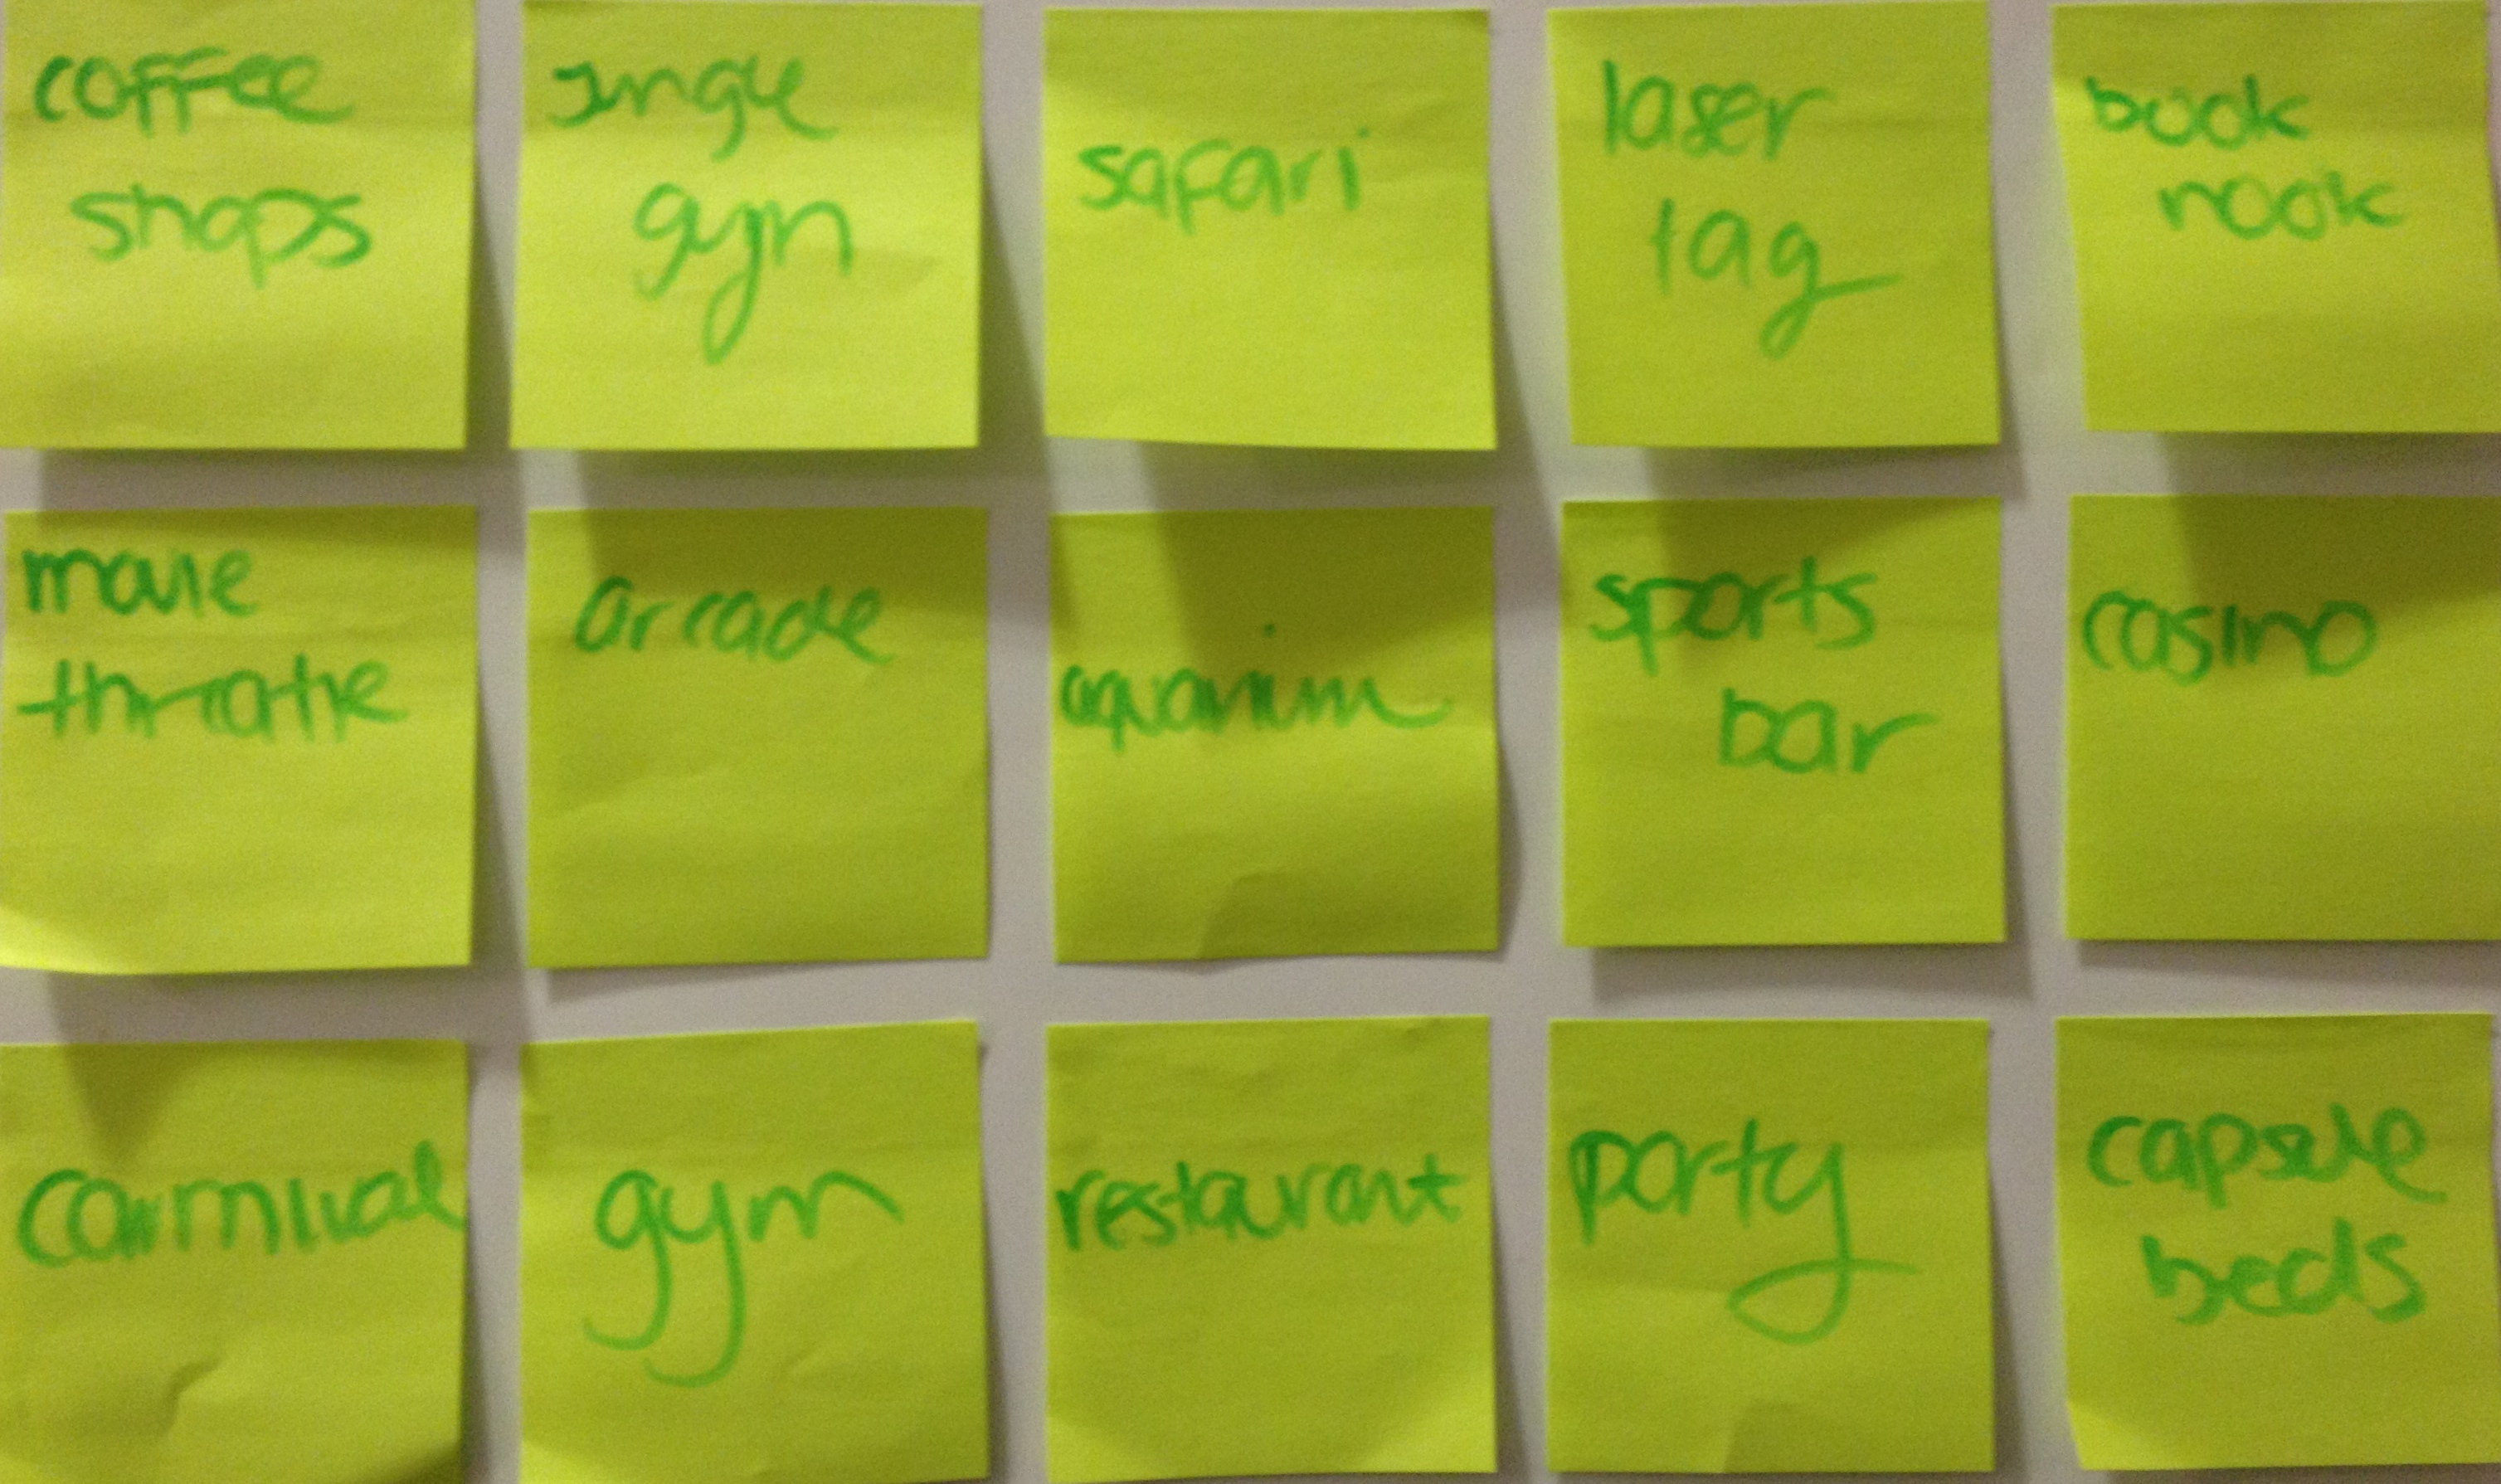
\includegraphics[width=7cm]{images/possible_themes.jpg}
   \caption{Possible ideas for a new cabin configuration}
  \label{fig:possible_themes.jpg}
\end{figure}

Our goal for the first Dark Horse Prototype was to find ways to make flying an enjoyable activity, not just another form of transportation. While many passengers find that getting to and around the airport, going through security, and waiting for a flight to board can be a waste of time and a draining activity, people are willing to pay to stand in line at theme parks for hours on end just to get on a fun ride for a few minutes or camp out outside of stores just to get the new iPhone. We believe that if we could make the flying experience a better one, passengers would be less bothered by the less-than-pleasant activities leading up to it. 

We realized that a redesigned cabin would need to be more accessible but could also have different sections explicitly to harness our users’ varied needs and reasons for flying. Flying tends to be a time for rest for many and because of this we researched what others had done to convert the cabin from a “sitting room only” configuration to a more sleep-friendly space. One of the proxies we looked at were the pod hotels in Japan, shown in Figure \ref{fig:hotel_pod.jpg}, where people sleep in fairly compact space-efficient pods. Similar pods could be designed for use in an airplane cabin, reappropriating room typically used for seating to sleeping spaces.

\begin{figure}[h]
  \centering
     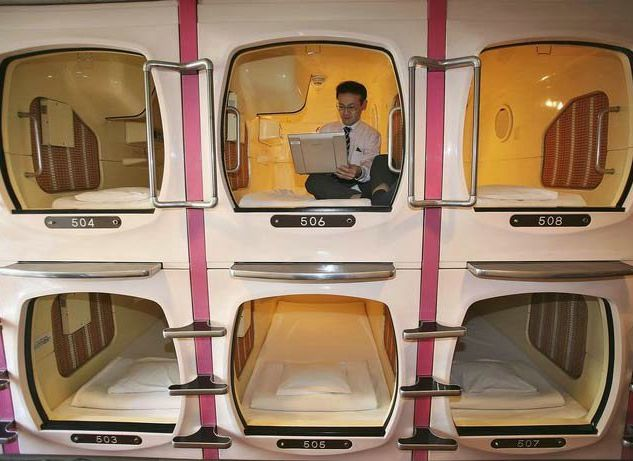
\includegraphics[width=7cm]{images/hotel_pod.jpg}
   \caption{Current pod hotel layout in Japan. \cite{hotel_pod}}
  \label{fig:hotel_pod.jpg}
\end{figure}

There are a number of possible airplane configurations for converting the whole airplane into beds. This could be done by utilizing the vertical space available in the cabin, as shown in Figures \ref{fig:blue_vertical_configuration.png} and \ref{fig:purple_vertical_configuration.png}. 

\begin{figure}[h]
  \centering
     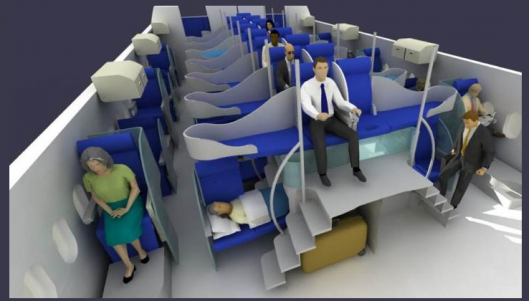
\includegraphics[width=7cm]{images/blue_vertical_configuration.png}
   \caption{Example of cabin layout that integrates both chairs and beds and does not decrease the total number of seats. \cite{blue_vertical} }
  \label{fig:blue_vertical_configuration.png}
\end{figure} 

\begin{figure}[h]
  \centering
     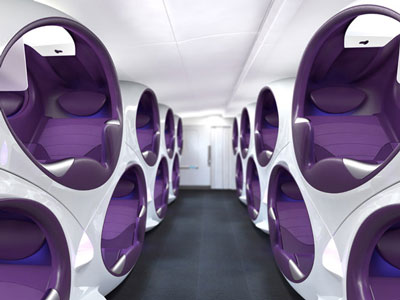
\includegraphics[width=7cm]{images/purple_vertical_configuration.jpg}
   \caption{Example of cabin layout with built in beds. \cite{purple_vertical}}
  \label{fig:purple_vertical_configuration.png}
\end{figure} 

These configurations make the flying experience much more comfortable while at the same time enabling selective seats to be much more accessible than others. These configurations would allow our users to easily get in and out of their seats without facing the problems they face today.

Our team also explored the possibility of sleeping while standing as opposed to laying down and found that there are several design firms that have been exploring vertical seating arrangements like the one shown in Figure \ref{fig:vertical_seating.jpg}. These designs have received a lot of backlash due to their perceived disregard for passenger comfort despite the fact that they may actually be better for our health. 

\begin{figure}[h]
  \centering
     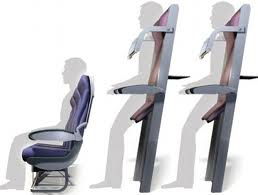
\includegraphics[width=7cm]{images/vertical_seating.jpg}
   \caption{Vertical seating being designed for airplane chairs. \cite{vertical_seating}}
  \label{fig:vertical_seating.jpg}
\end{figure} 

We know that many of our users travel for work purposes so we also considered what the best places to comfortably do work are and found that many preferred coffee shops to their offices. Our team also thought about having a gym integrated during the flight, transforming that seemingly lost flight time into a productive workout. Finally, we looked at different products available for creating a more accessible experience, including handles, conveyor belts and revolving doors. From all of this research, we created our first Dark Horse prototypes.

\subsection{Description of the prototype}
In order to make our users think about the present and not only their future destination we wanted to build a flexible and dynamic cabin layout enabling a more customized flight experience for everyone, especially handicapped passengers. \\

We made the assumption that when passengers buy their tickets, they will have to go through a questionnaire asking them for their preferred activity during the flight. According to their answers they will be placed in the appropriate section of the plane and have the opportunity to do what they really want to do during the flight. If the passengers have special needs due to physical handicaps, we wanted each of our different sections to address these issues and improve the experience not only for everyone, but in particular for those with reduced mobility. \\

Our team decided to focus on the design of 5 main sections and built a dynamic scale model for each one:

\subsubsection{Sleeping Area}
We wanted our user to be able to rest and relax so we thought of different types of beds or resting pods as mentioned in the benchmarking section. However, when we tried to prototype them and build our scale model we found at that it was quite hard to keep the number of seats the same. In order to not violate this constraint, our team decided to explore solutions that require a very limited space. As such, we designed our sleeping section with foldable seats which can be unfolded to become a bed as shown on the next picture.

\begin{figure}[h]
  \centering
     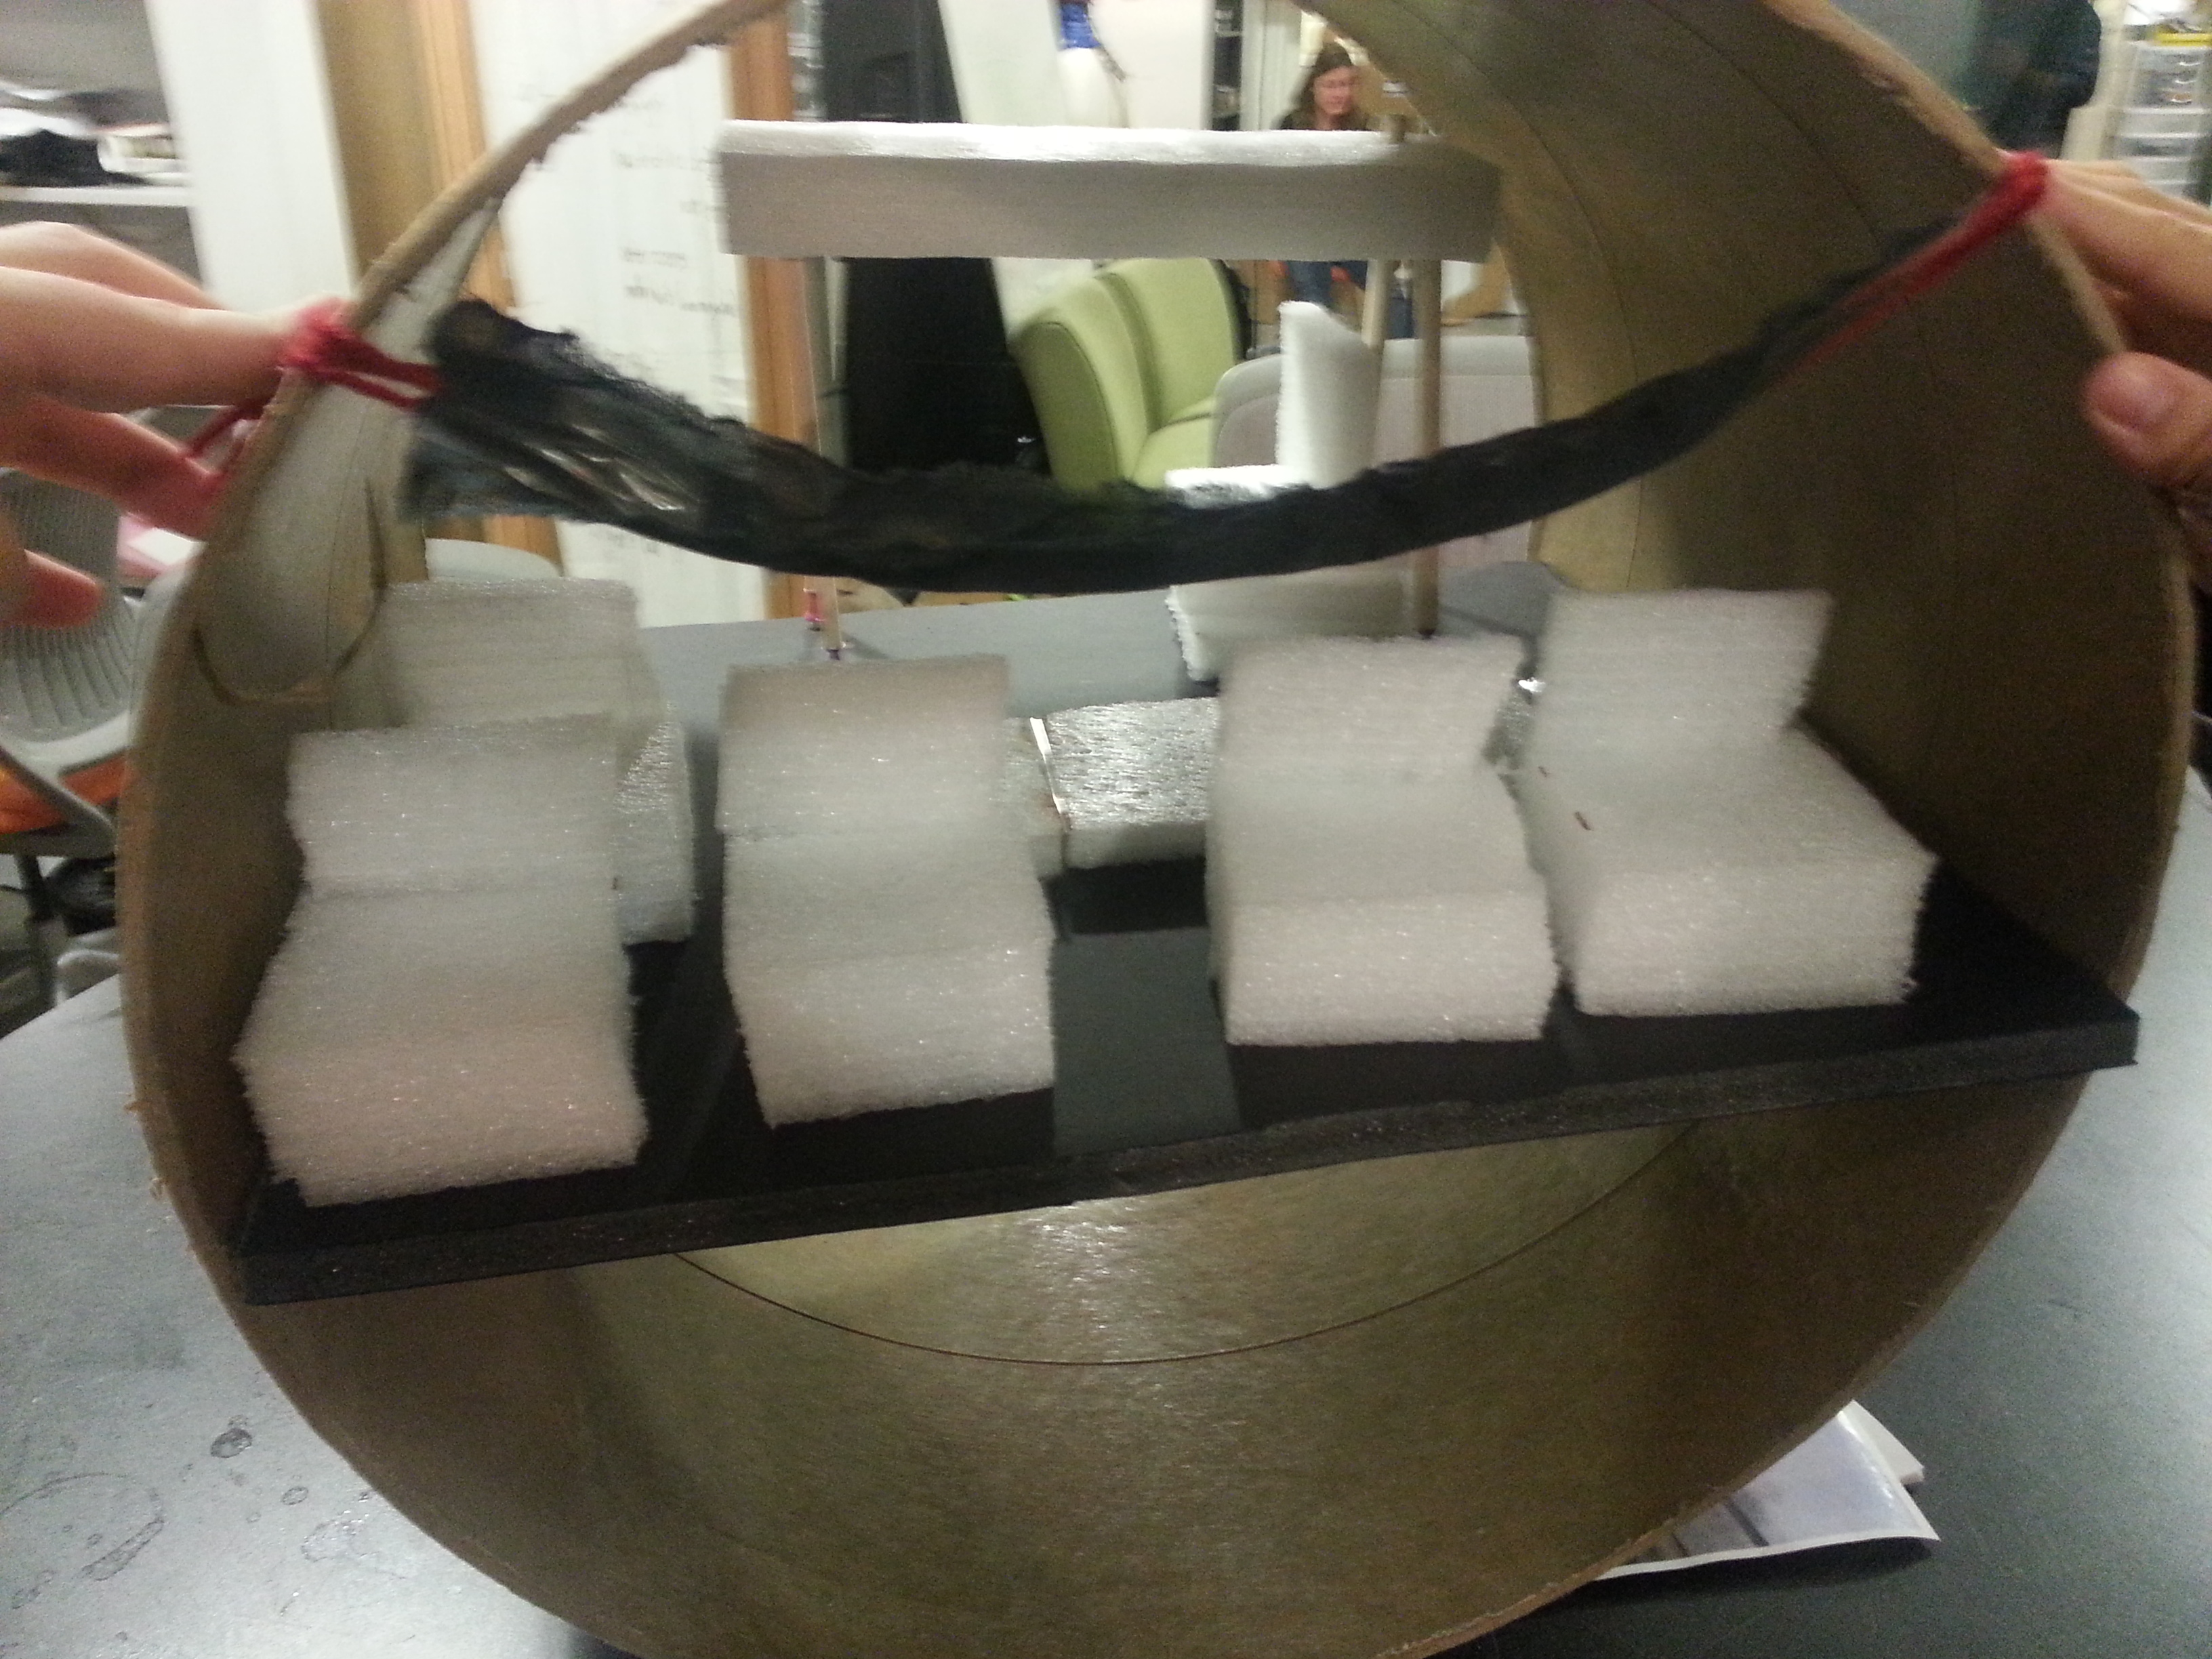
\includegraphics[width=7cm]{images/20140116_172733.jpg}
   \caption{Plane section dedicated to sleep and relaxation with two configurations: take-off/landing (left) and cruise (right)}
  \label{fig:20140116_172733}
\end{figure}

We also studied the possibility of using hammocks but the available space in the cabin was not sufficient to make it work.

\subsubsection{Family Area}
When talking about passengers with reduced mobility people generally picture wheelchair users and passengers with other physical handicaps, but in a sense, families with young children and pregnant women also have reduced mobility compared to the average passenger. In order to address their specific needs our team designed an entire section of the plane to be the family compartment.

We designed this section to be flexible and easily adaptable to family needs. If parents want to sit close to their children and look after them they can get rid of the armrests and convert their row of seats into a sort of bench allowing the family to stay together during the flight. In order to make it easier for parents, children and pregnant women to move through this area we coupled our idea of a bench with the design of a retractable table that can be folded and unfolded between two consecutive rows of seats facing each other. When the table is unfolded it is then easier for people on the benches to access the aisle as shown on the following pictures. 

\begin{figure}[h]
  \centering
     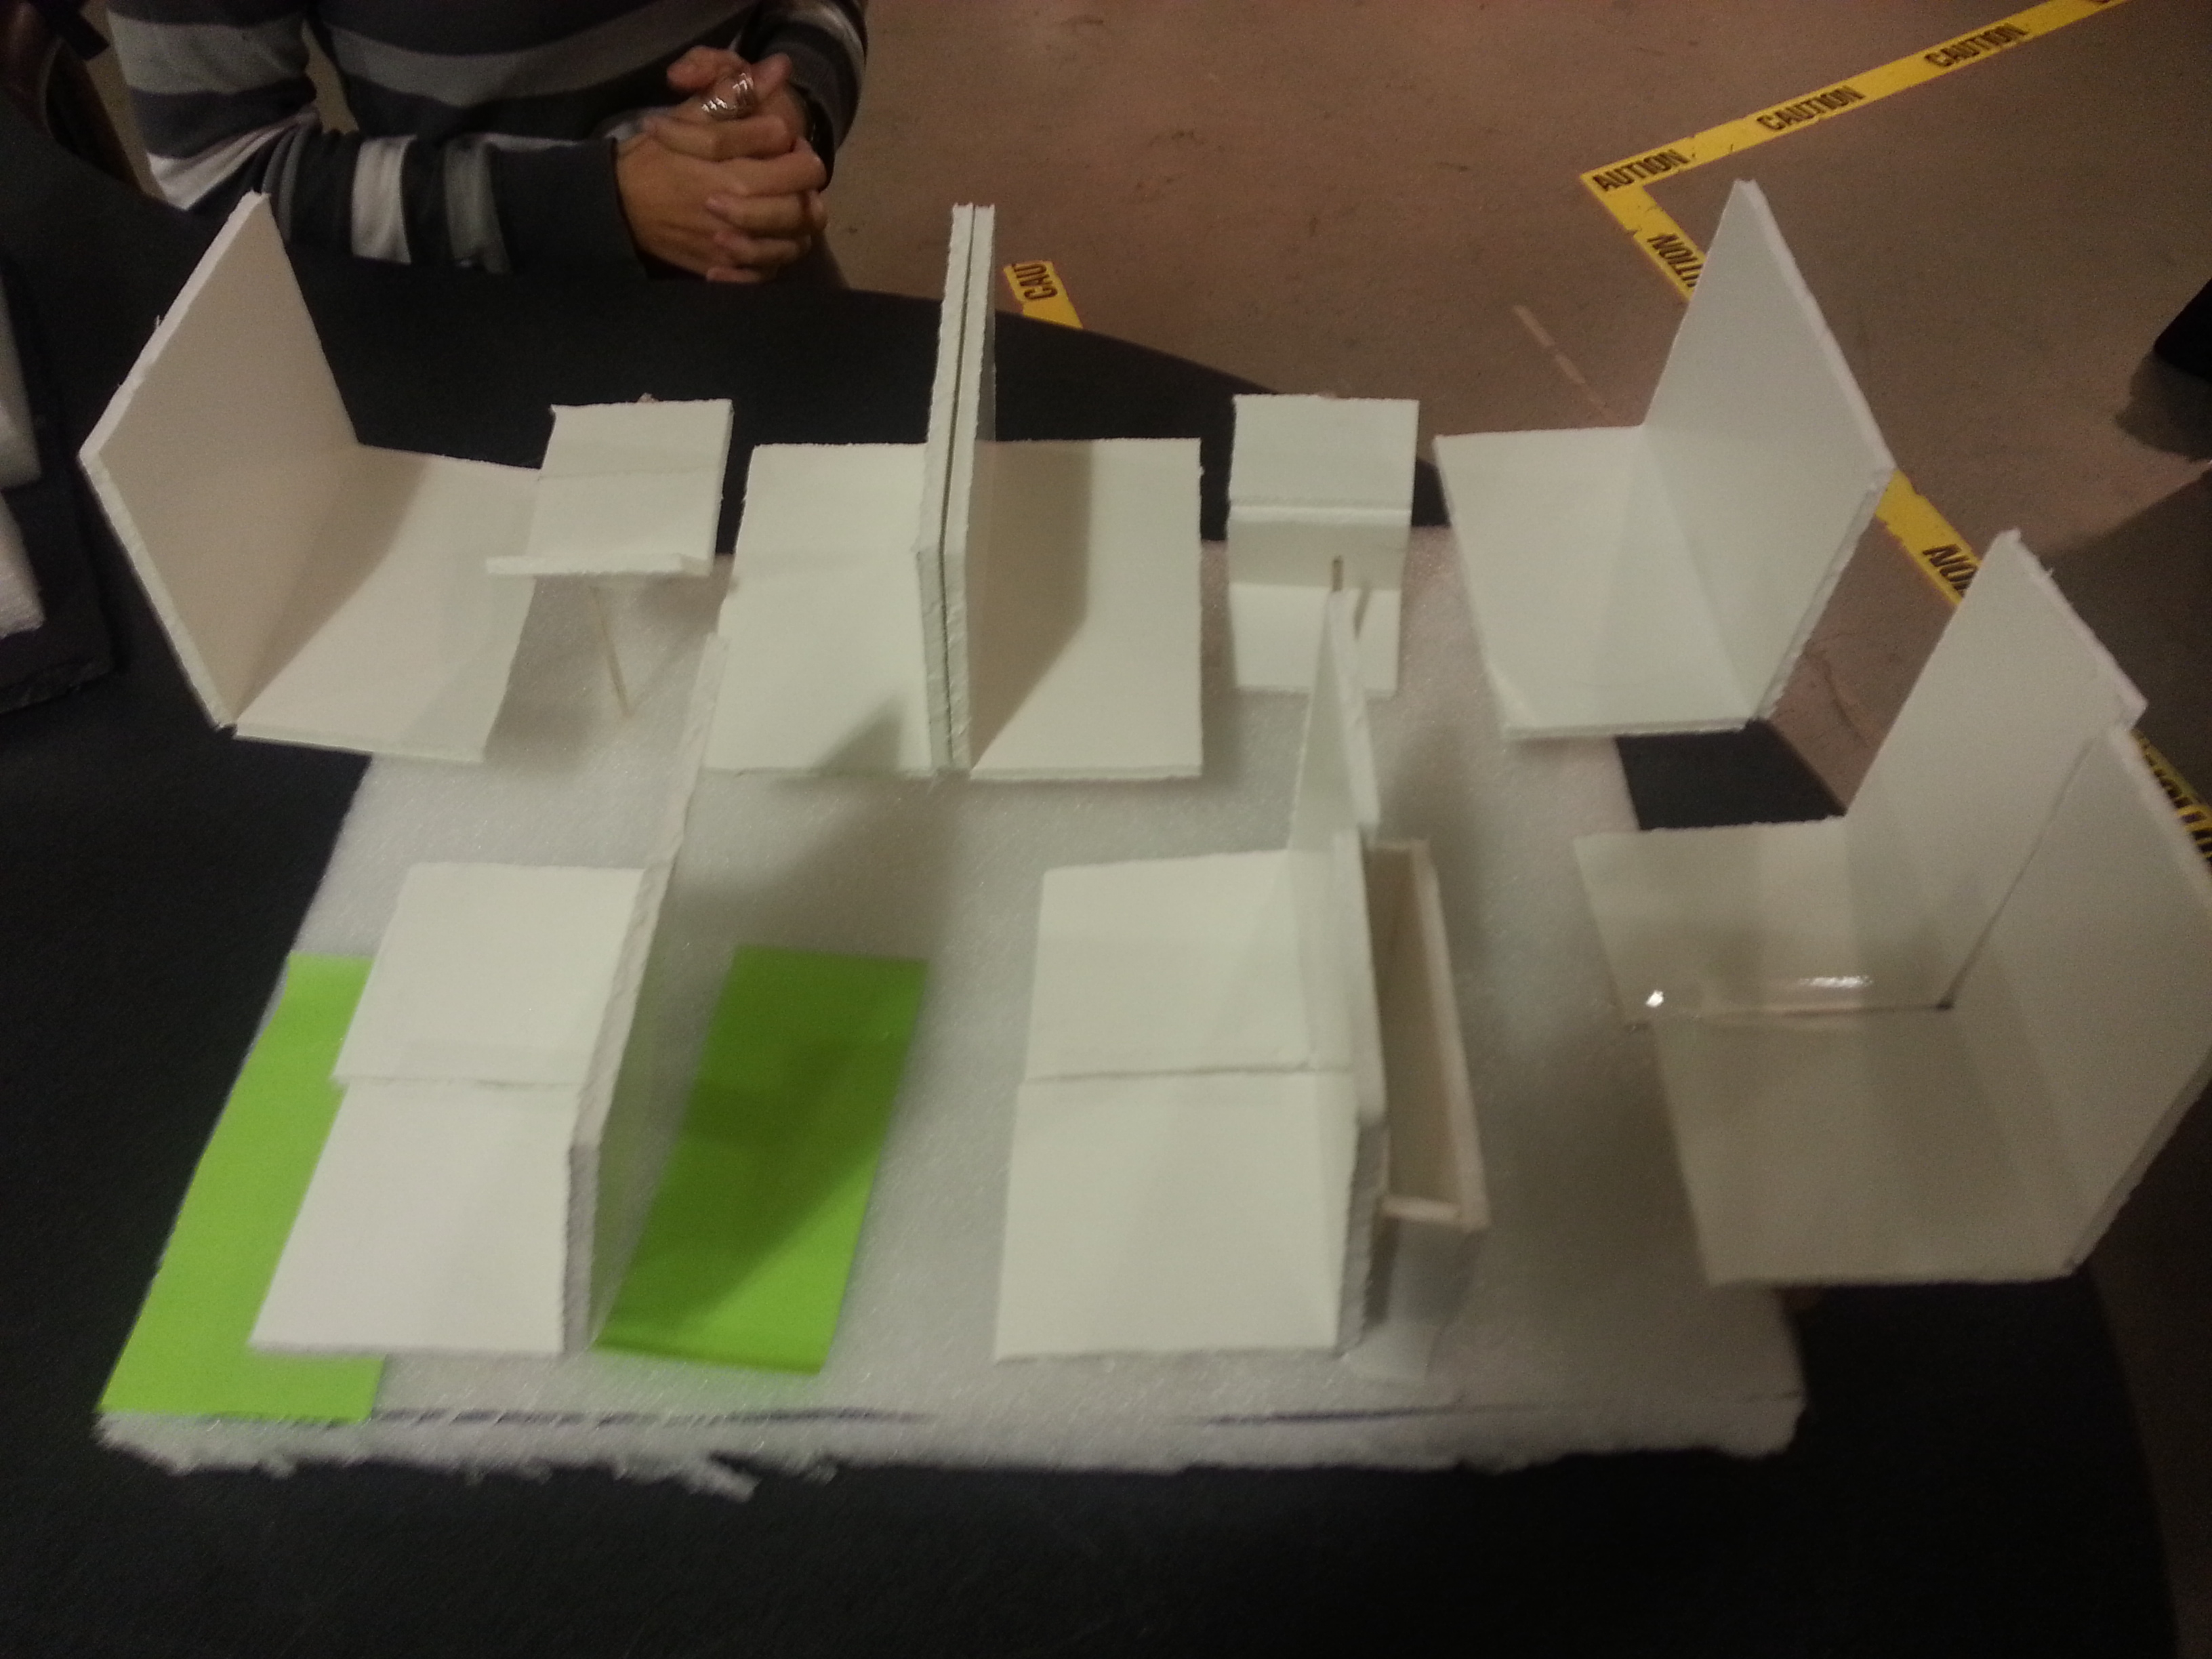
\includegraphics[width=7cm]{images/20140116_173112.jpg}
   \caption{Plane section dedicated to family with two configurations: take-off/landing (left) and cruise (right)}
  \label{fig:20140116_173112}
\end{figure}

We also considered the fact that the family section of the plane could be sound proof in order to prevent disturbances to the sleeping compartment and concentrate the noise of children playing together in one single area.

\subsubsection{Gym Area}
When our team brainstormed about what people would like to do during their flight we thought that being able to move your limbs and stretch was a big issue, especially for people with blood circulation problems. In order to solve that we thought that having convertible seats that can be turned into yoga mats or that can be used as gym accessories could improve our user’s experience. We imagined a cabin layout that is standard for takeoff and landing but that can be turned into a gym area during the cruise, as displayed in the figures below. \\

\begin{figure}[h]
  \centering
     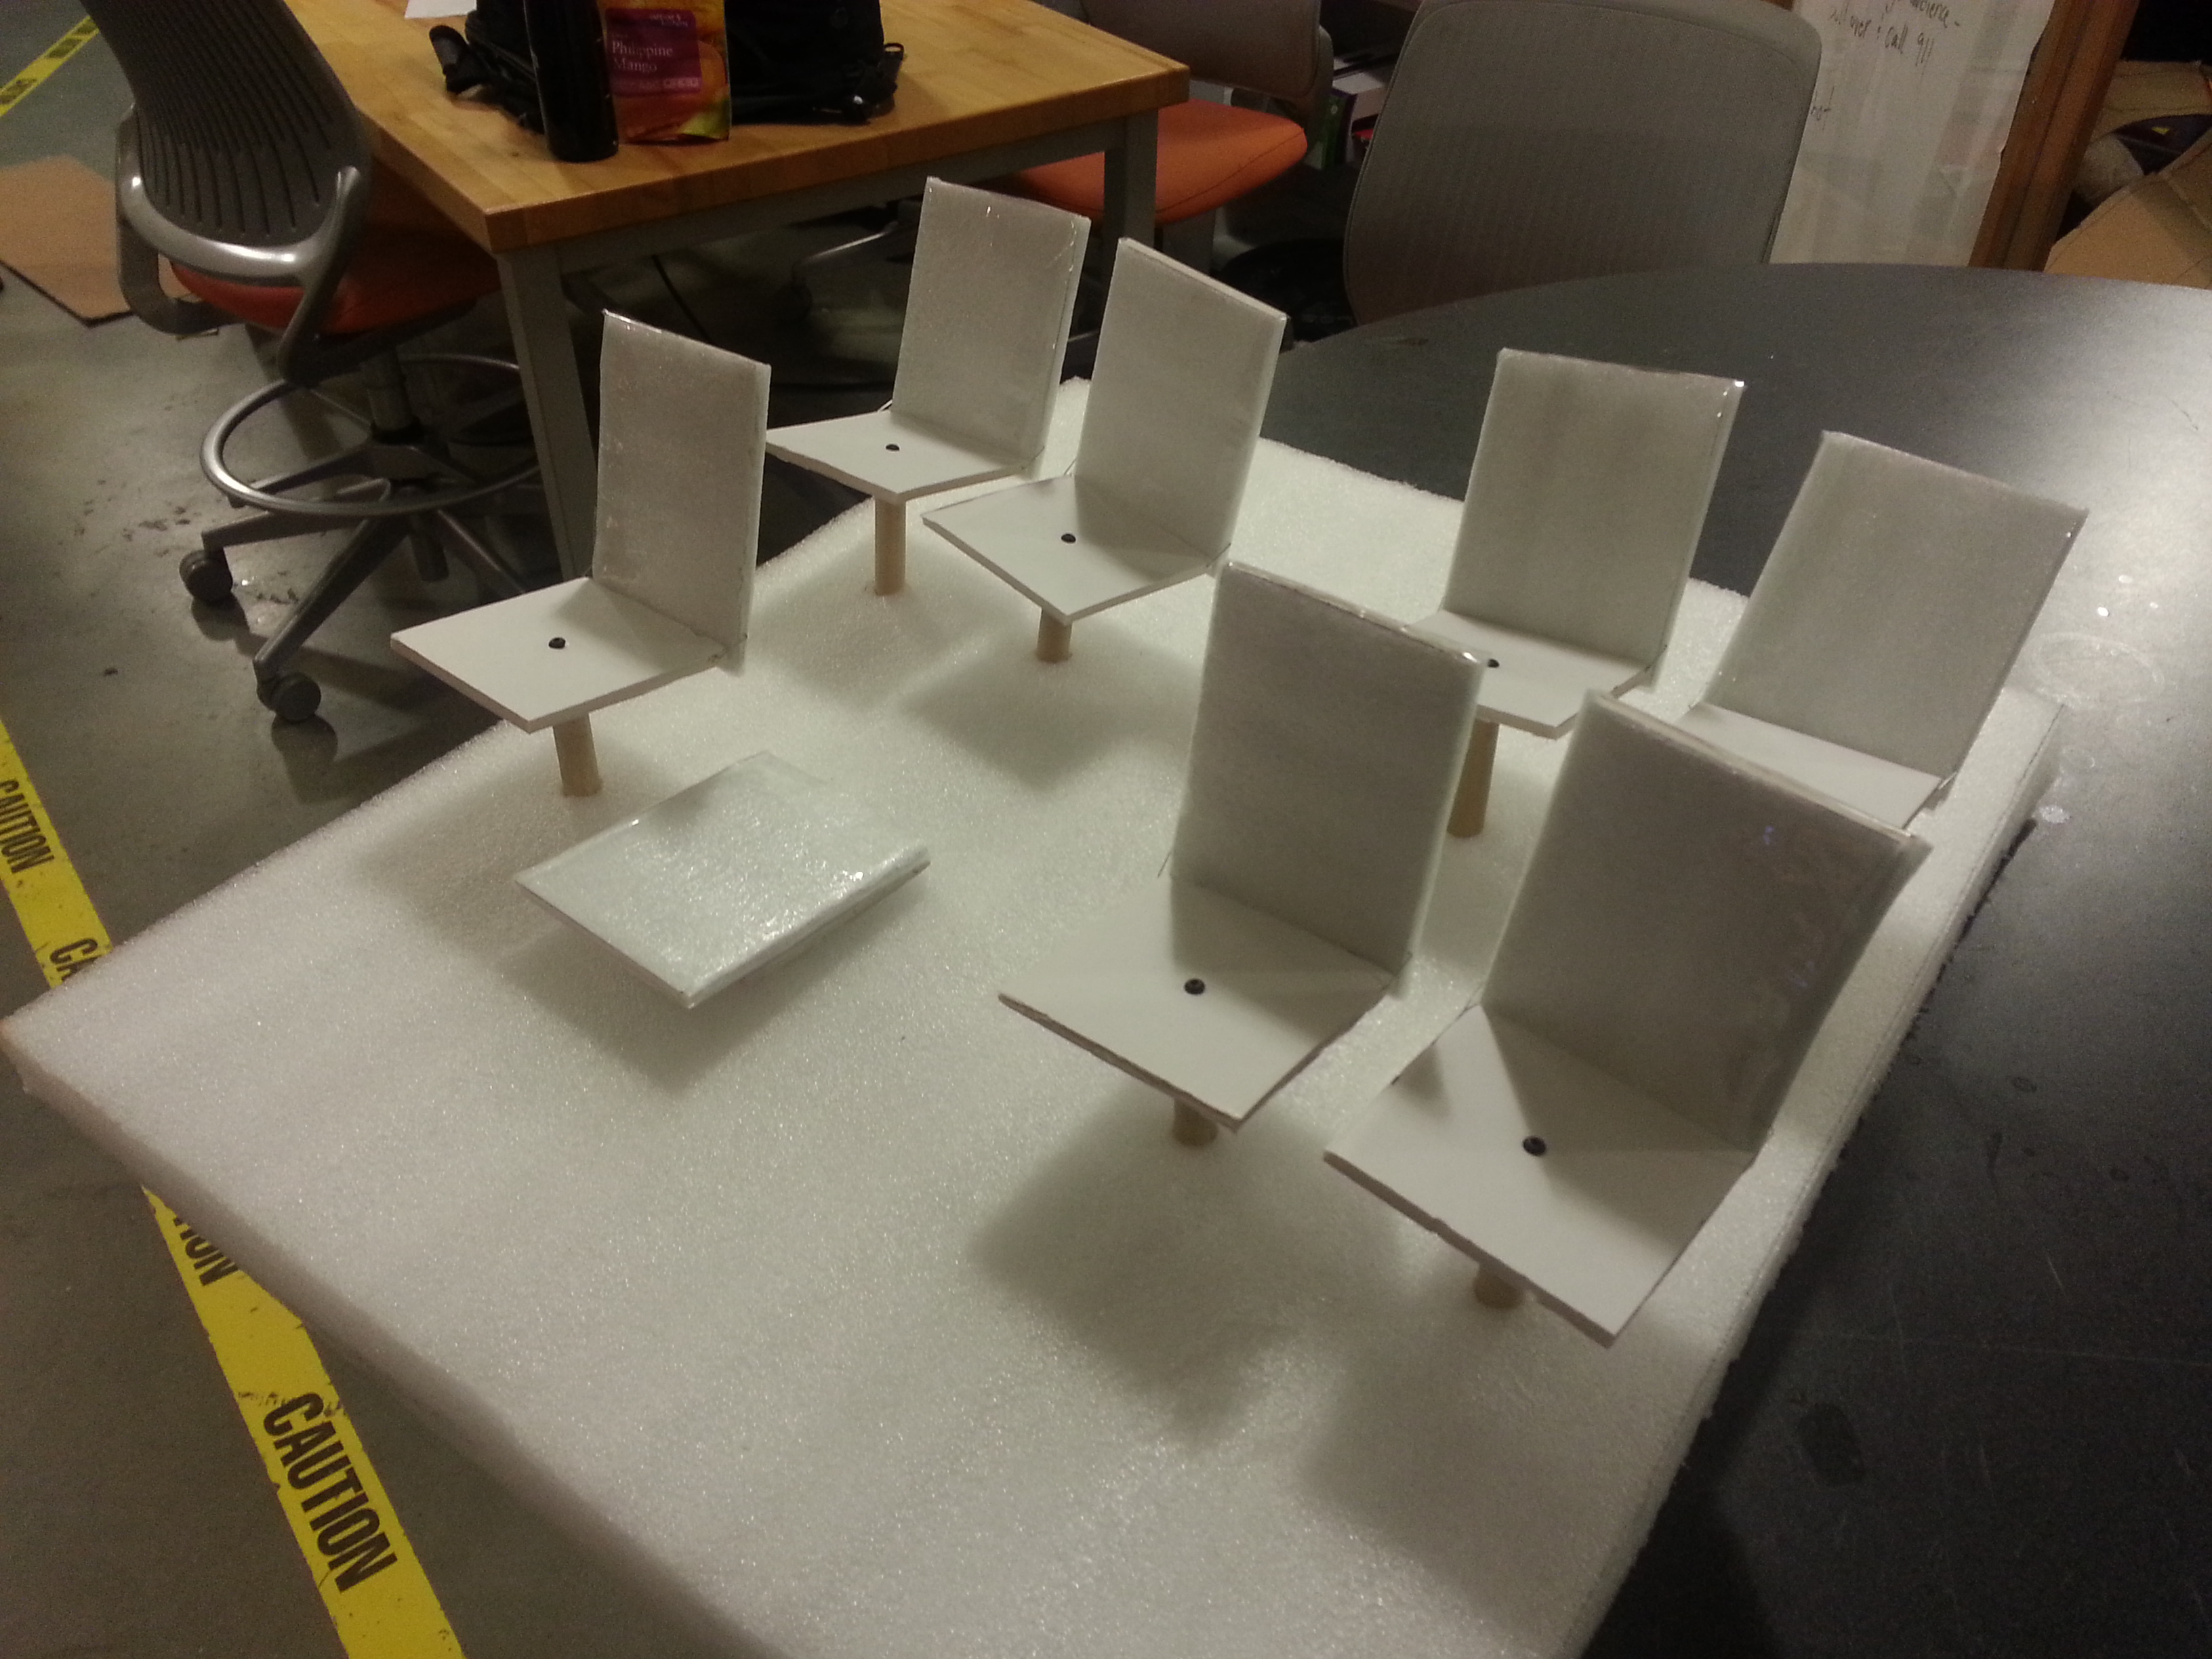
\includegraphics[width=7cm]{images/20140116_172402.jpg}
   \caption{Plane section dedicated to sports and physical training with two configurations: take-off/landing (left) and cruise (right)}
  \label{fig:20140116_172402}
\end{figure}

People with reduced mobility sometimes need to do physical therapy (PT) exercises to avoid blood circulation issues. However, handicapped people can rarely do their PT exercises alone so it’s possible that flight attends could be trained specifically to assist these passengers.

We also took into account the fact that people are often thirsty due to perspiration when they are physically active so we thought about a system of individual straws that would be available in each passenger’s space allowing to drink water whenever they want without having to call the flight attendants or move across the cabin. This idea can also be extended to all the sections and all the passengers allowing them to feel more in control and more independent.

\subsubsection{Book Nook}
Since a lot of people, including those with reduced mobility, travel by plane for professional reasons our team wanted to design a plane section that imitates the cosy atmosphere of a coffee shop where people feel relaxed and comfortable while working.
To do so we imagined convertible seats that can be turned into couches and provide better support for people with reduced mobility. 

\begin{figure}[h]
  \centering
     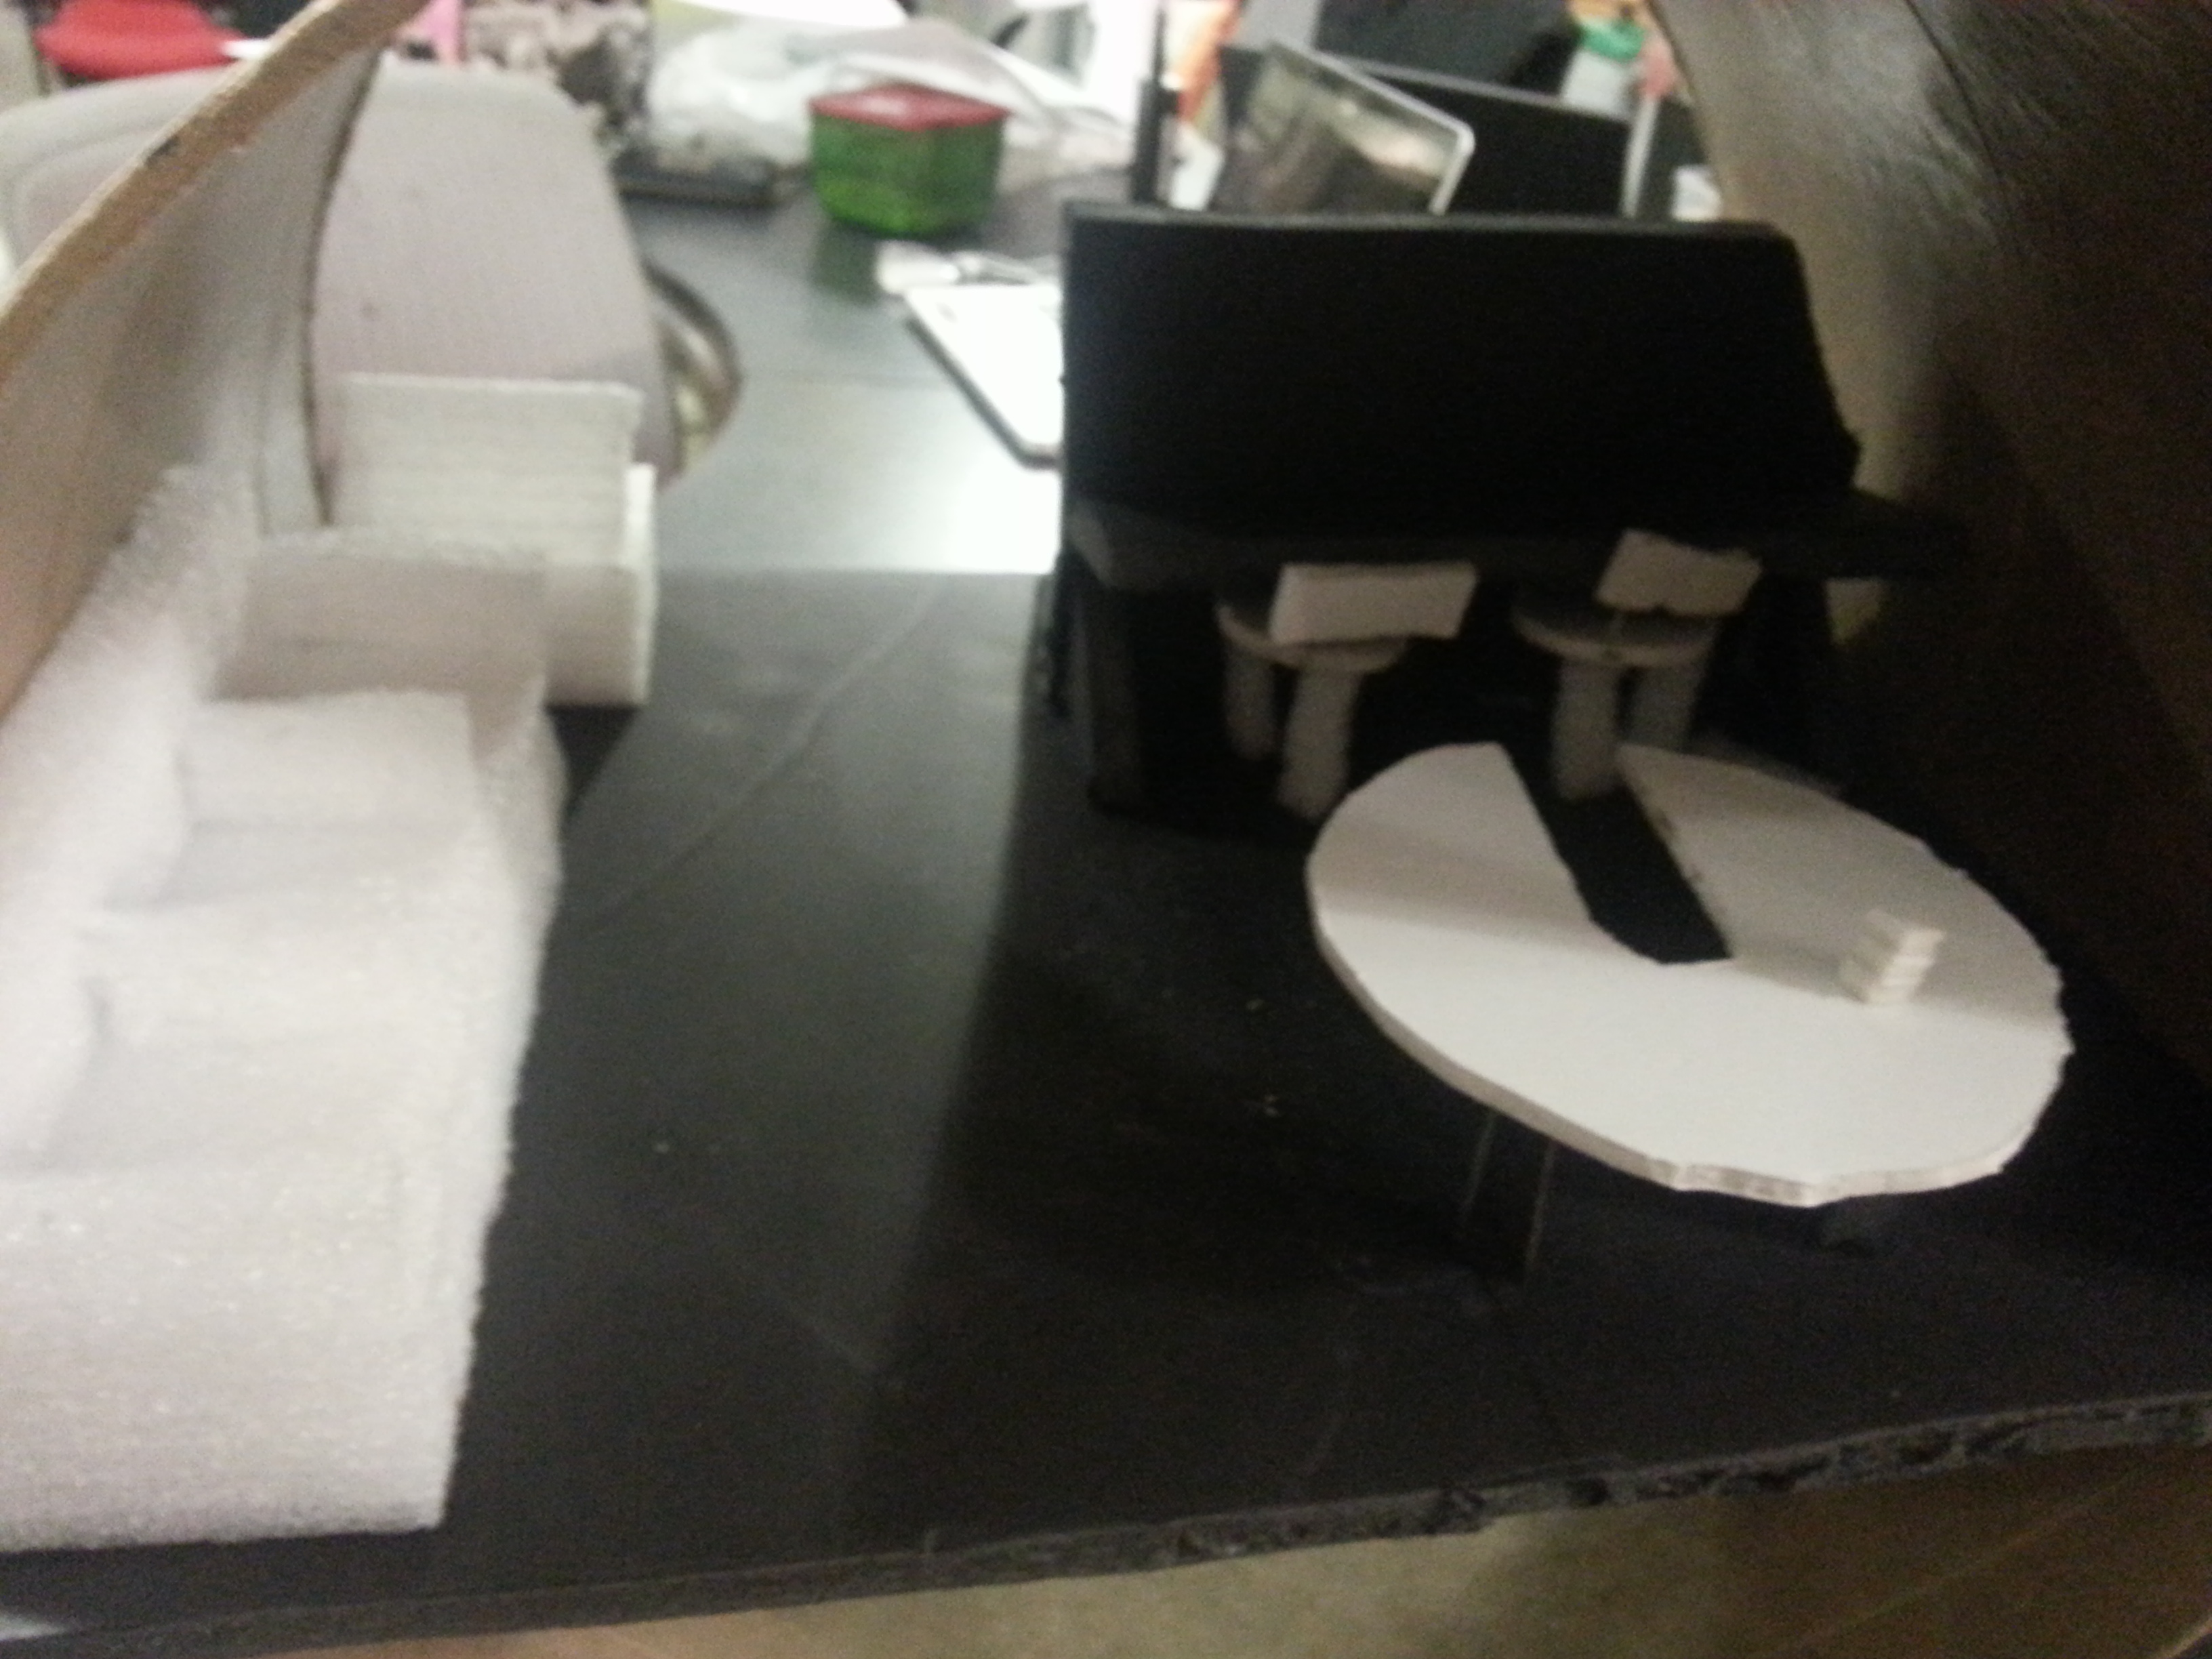
\includegraphics[width=7cm]{images/20140116_172928.jpg}
   \caption{Plane section dedicated to work in a cosy atmosphere with two configurations: take-off/landing (left) and cruise (right)}
  \label{fig:20140116_172928}
\end{figure}

We also thought that having a round table with one or two flight attendants in the center providing drinks was a good way to have them closer to passengers requiring more attention and assistance.

\subsubsection{Ease of Access - Carousel}
We decided to fully dedicate the last plane section we designed to people with reduced mobility. In the previous sections we addressed their issues by trying to improve everyone experience so that handicapped people would not feel segregated, but for this last section we focused specifically on their needs and expectations. 
Our team found out that boarding and disembarking from the plane and moving in/out of their seats were the biggest issues for passengers with reduced mobility. In order to improve this part of their flight experience, our team decided to get rid of the current cabin layout where seats are lined up. 

We wanted to explore a different configuration where the seats are part of a carousel system that rotates so that any time a passenger enters the aircraft the seat right in front of them is empty. This would limit the distance people have to cover to get to their seat and should make it easier for them to move in/out of their seat since there is no obstacle in front of them as shown in the following pictures.

\begin{figure}[h]
  \centering
     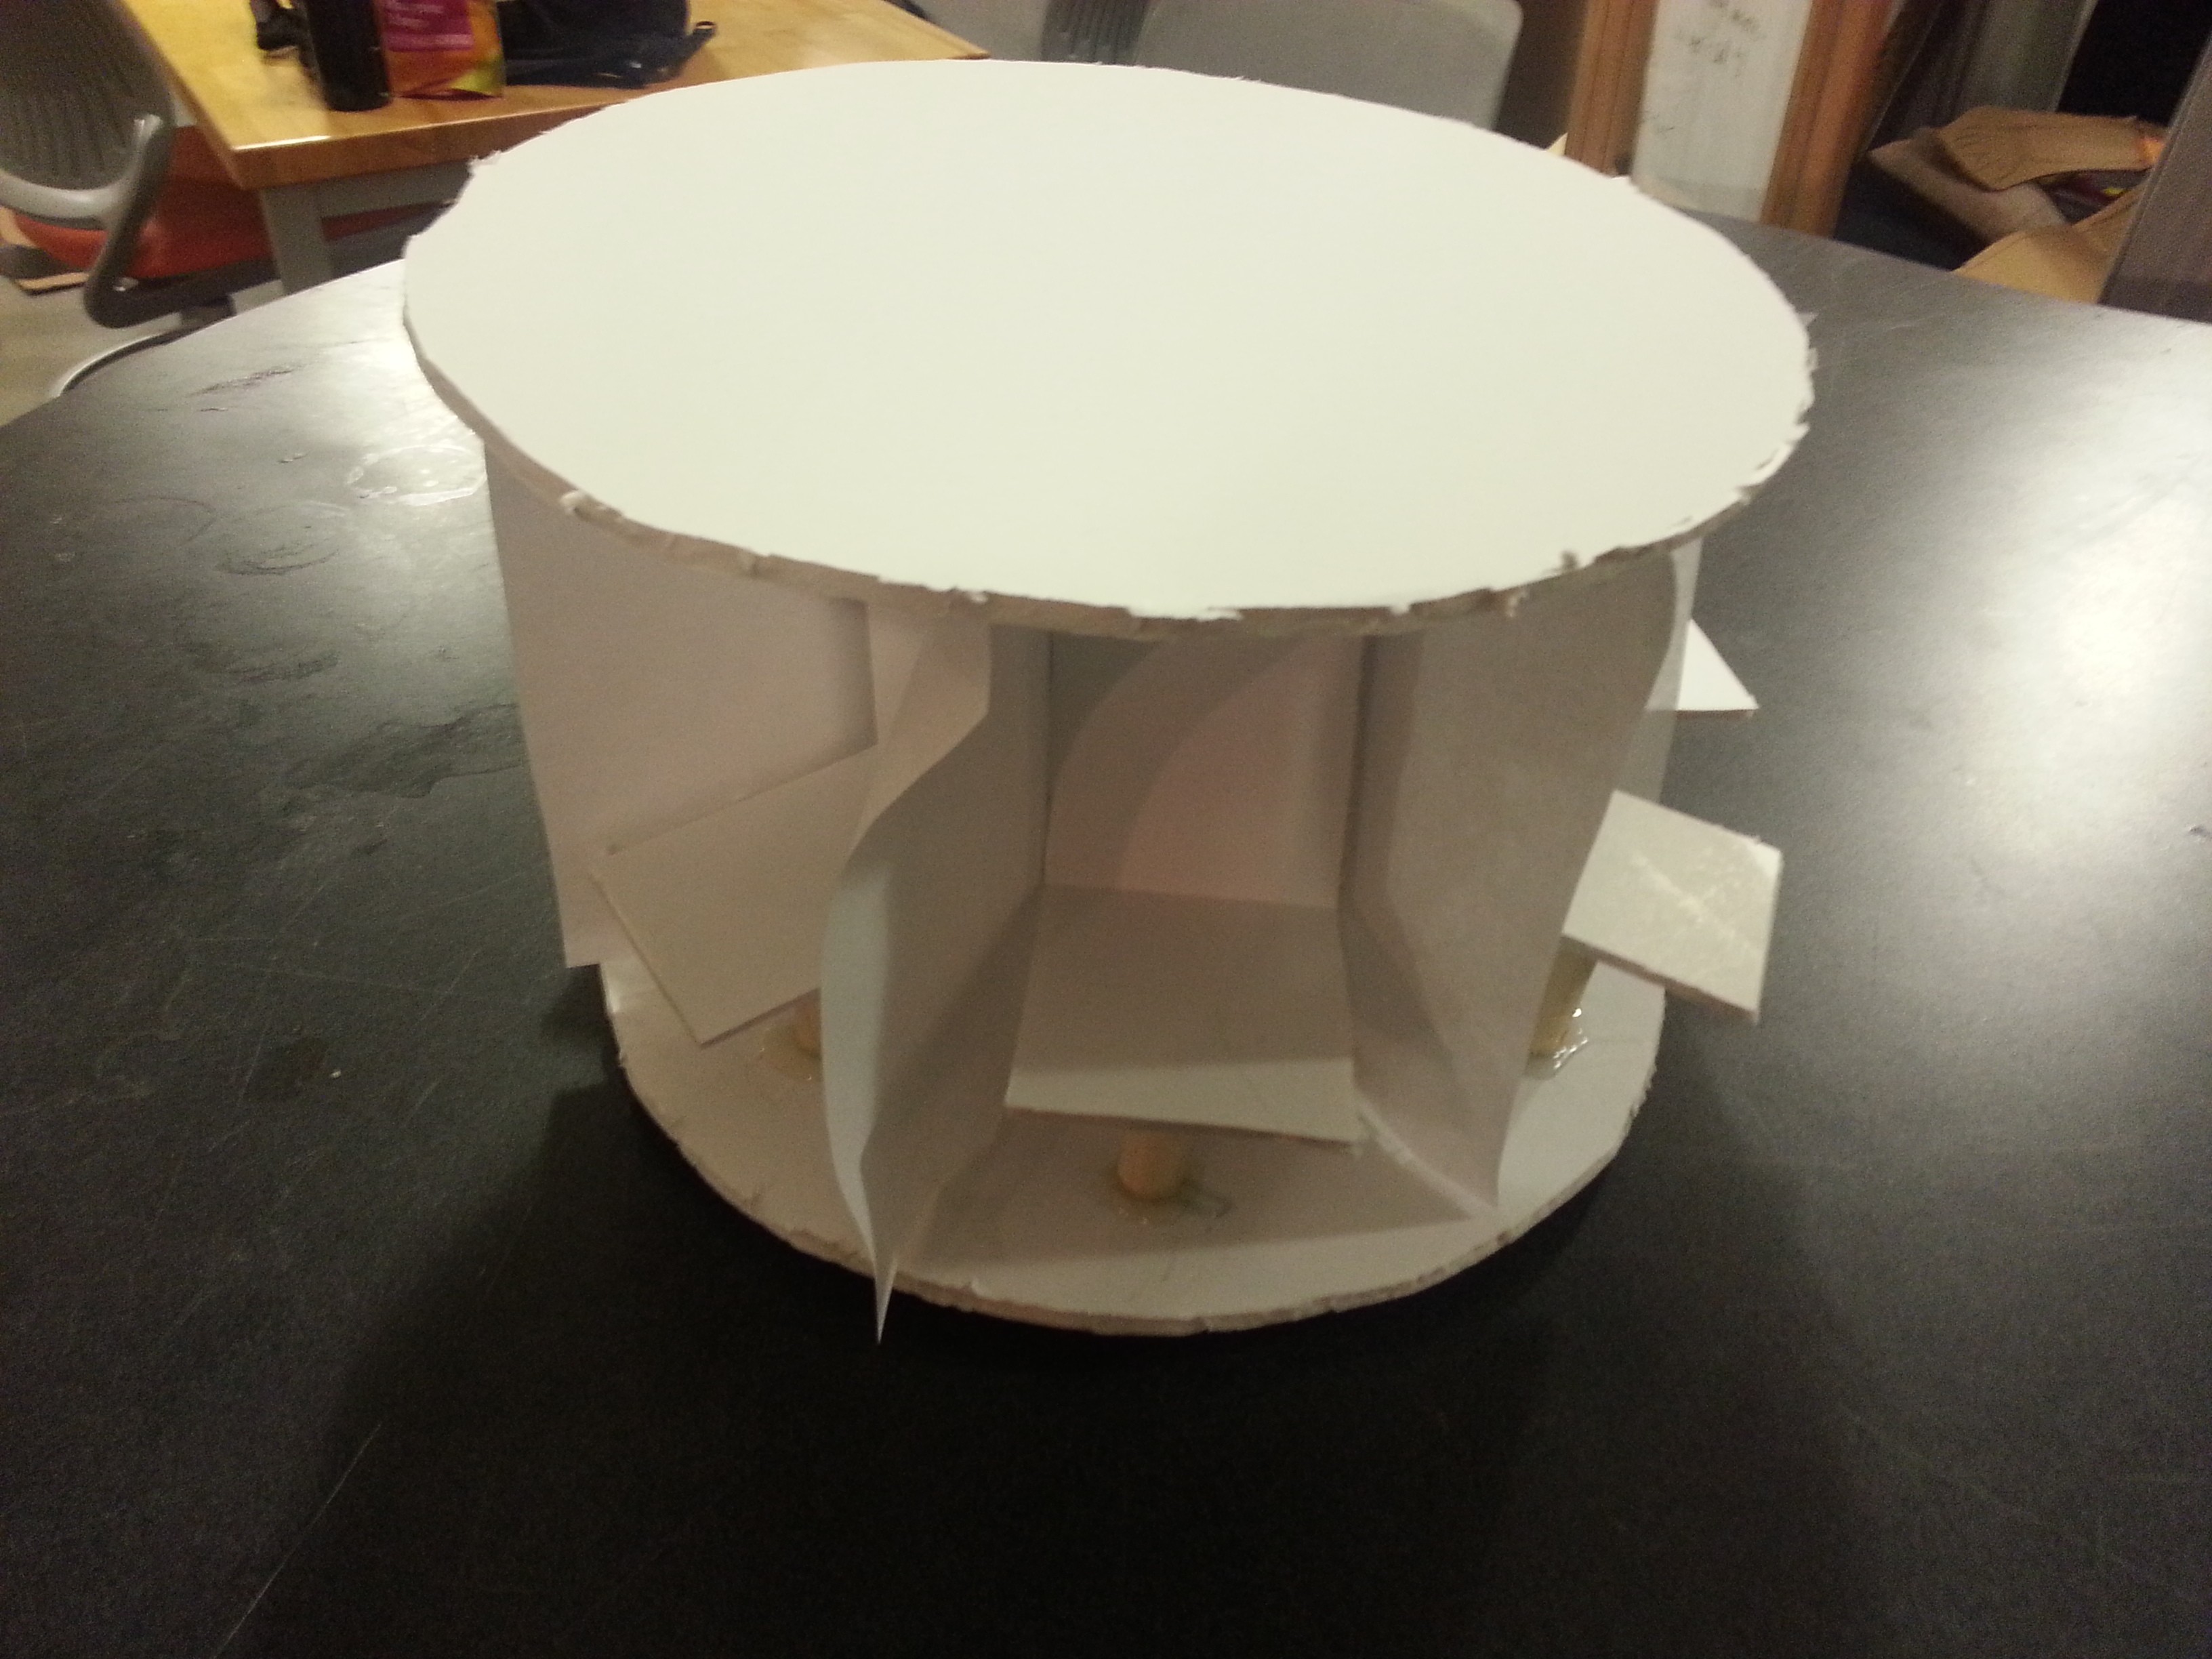
\includegraphics[width=7cm]{images/20140116_172516.jpg}
   \caption{Plane section dedicated to people who need easily accessible seats}
  \label{fig:20140116_172516}
\end{figure}

We also thought that one of the seats from the carousel could be removed from the circle, making the center of the system accessible. If the central part of the carousel can be accessed then it could be used as a place where wheelchairs or other equipment could be stored.


\subsection{Learnings}
\begin{enumerate}
	\item The following learnings came as a result of team discussions, analysis, and feedback from the teaching team. 
	\item It is difficult to reconfigure the cabin without losing seats. However, to maximize profit airlines do not want to lose any seats, making it important to maintain the same number.
	\item The number of possible cabin configurations increase with the implementation of dynamic seats.  Dynamic seats will allow for movement of cabin sections to meet the demands of each passenger. 
	\item Personalizing the flight would improve the experience for all passengers, not just disabled passengers. Many passengers compare the boarding and flight experience to the herding of cattle. By allowing passengers to choose their prefered cabin surrounding or configuration, they play a role in their experience and have more control over their situation. 
	\item Flight attendants may be able to play different roles in the passengers’ experiences.  They would be able to cater more toward what a passenger wants instead of performing a wide range of services for all passengers who might not need or want a certain service. 
	\item Every cabin configuration that can be implemented needs to have accessible features to fit the wide range of users our project encompasses.  The new cabin configurations cannot neglect our target user and should not make them feel singled out. 
\end{enumerate}

\section{Dark Horse Version 2}
\subsection{Benchmarking}
Our learnings from version 1 inspired us to continue to explore changing the cabin layout while also putting additional emphasis into the boarding process. We realized that if we could make the seats more accessible, we would be able to alleviate some of the pain brought on by the transfer process into today’s chairs. We looked at cabin configurations like the one in Figure \ref{fig:cabin_against_wall.jpg} where the seats face toward the inside of the cabin as opposed to the front. By having the seat face the passenger, it would be much easier to get in without having to worry about climbing over armrests or other passengers. 

\begin{figure}[h]
  \centering
     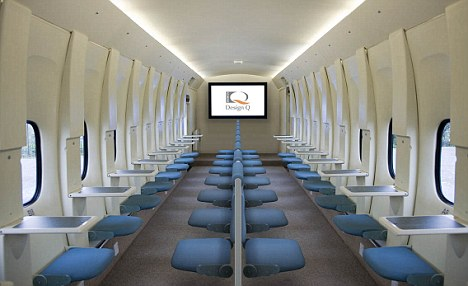
\includegraphics[width=7cm]{images/cabin_against_wall.jpg}
   \caption{Proposed cabin configuration where passengers are forced to be against the wall and face each other which increases the amount of passengers an aircraft can carry. \cite{vertical_seating} } %its the same website as the previous picture
  \label{fig:cabin_against_wall.jpg}
\end{figure} 

The team researched this further and found that seats are configured to be faced either toward the front or back for safety reasons relating to the forces that passengers could experience during flight. Having seats face inward could subject passengers to excessive lateral forces. Additionally, from the public reception of the configuration shown in Figure \ref{fig:cabin_against_wall.jpg},  we found that passengers would not feel comfortable directly facing other passengers. Thus, we looked at different types of boarding mechanisms that would enable a simpler boarding experience but that would also retain the safety level found in airplanes today. 

\subsection{Description}
In order to solve the problems faced by mobility challenged passengers we tried to radically change the boarding experience for everyone. To this end, our team decided to further investigate carousel concept developed in dark horse version 1 and push it to the extreme.

In order to go as far as possible with this concept we decided to:

 \begin{easylist}[itemize]

& Rethink the whole boarding process from the gate to the seat by creating a carousel inspired by a conveyor belt system through the entire plane.

& Design for an extreme case: a person with no mobility, i.e. a passenger without the use of any limbs. It made our mission more challenging but we thought it could be a good way to make sure we do not overestimate what a people with reduced mobility can or cannot do. In order to reach our goal, we brought a new persona: a mannequin filled with sand to mimic the weight of a real person.

\end{easylist}

We wanted our new persona to go through all the steps of the brand new boarding process we imagined:

\begin{easylist}[itemize]

& Waiting in line at the airport gate where position in the line is determined by seat number. This will facilitate the boarding process since people will have to board in the order defined by the cabin layout. Those in the aft of the plane would go first.

& While waiting, our new persona would be transferred to an airport chair that will then facilitate the transfer to the seat.

& When boarding starts, our persona will use a transfer mechanism located in the front of the cabin to reach his or her seat. Here are different options we modeled:

 \begin{easylist}[itemize]
	& The \textbf{hammock}-type transfer involves a seat that is detachable and can be moved from one chair to another using a lift
\begin{figure}[h]
  \centering
     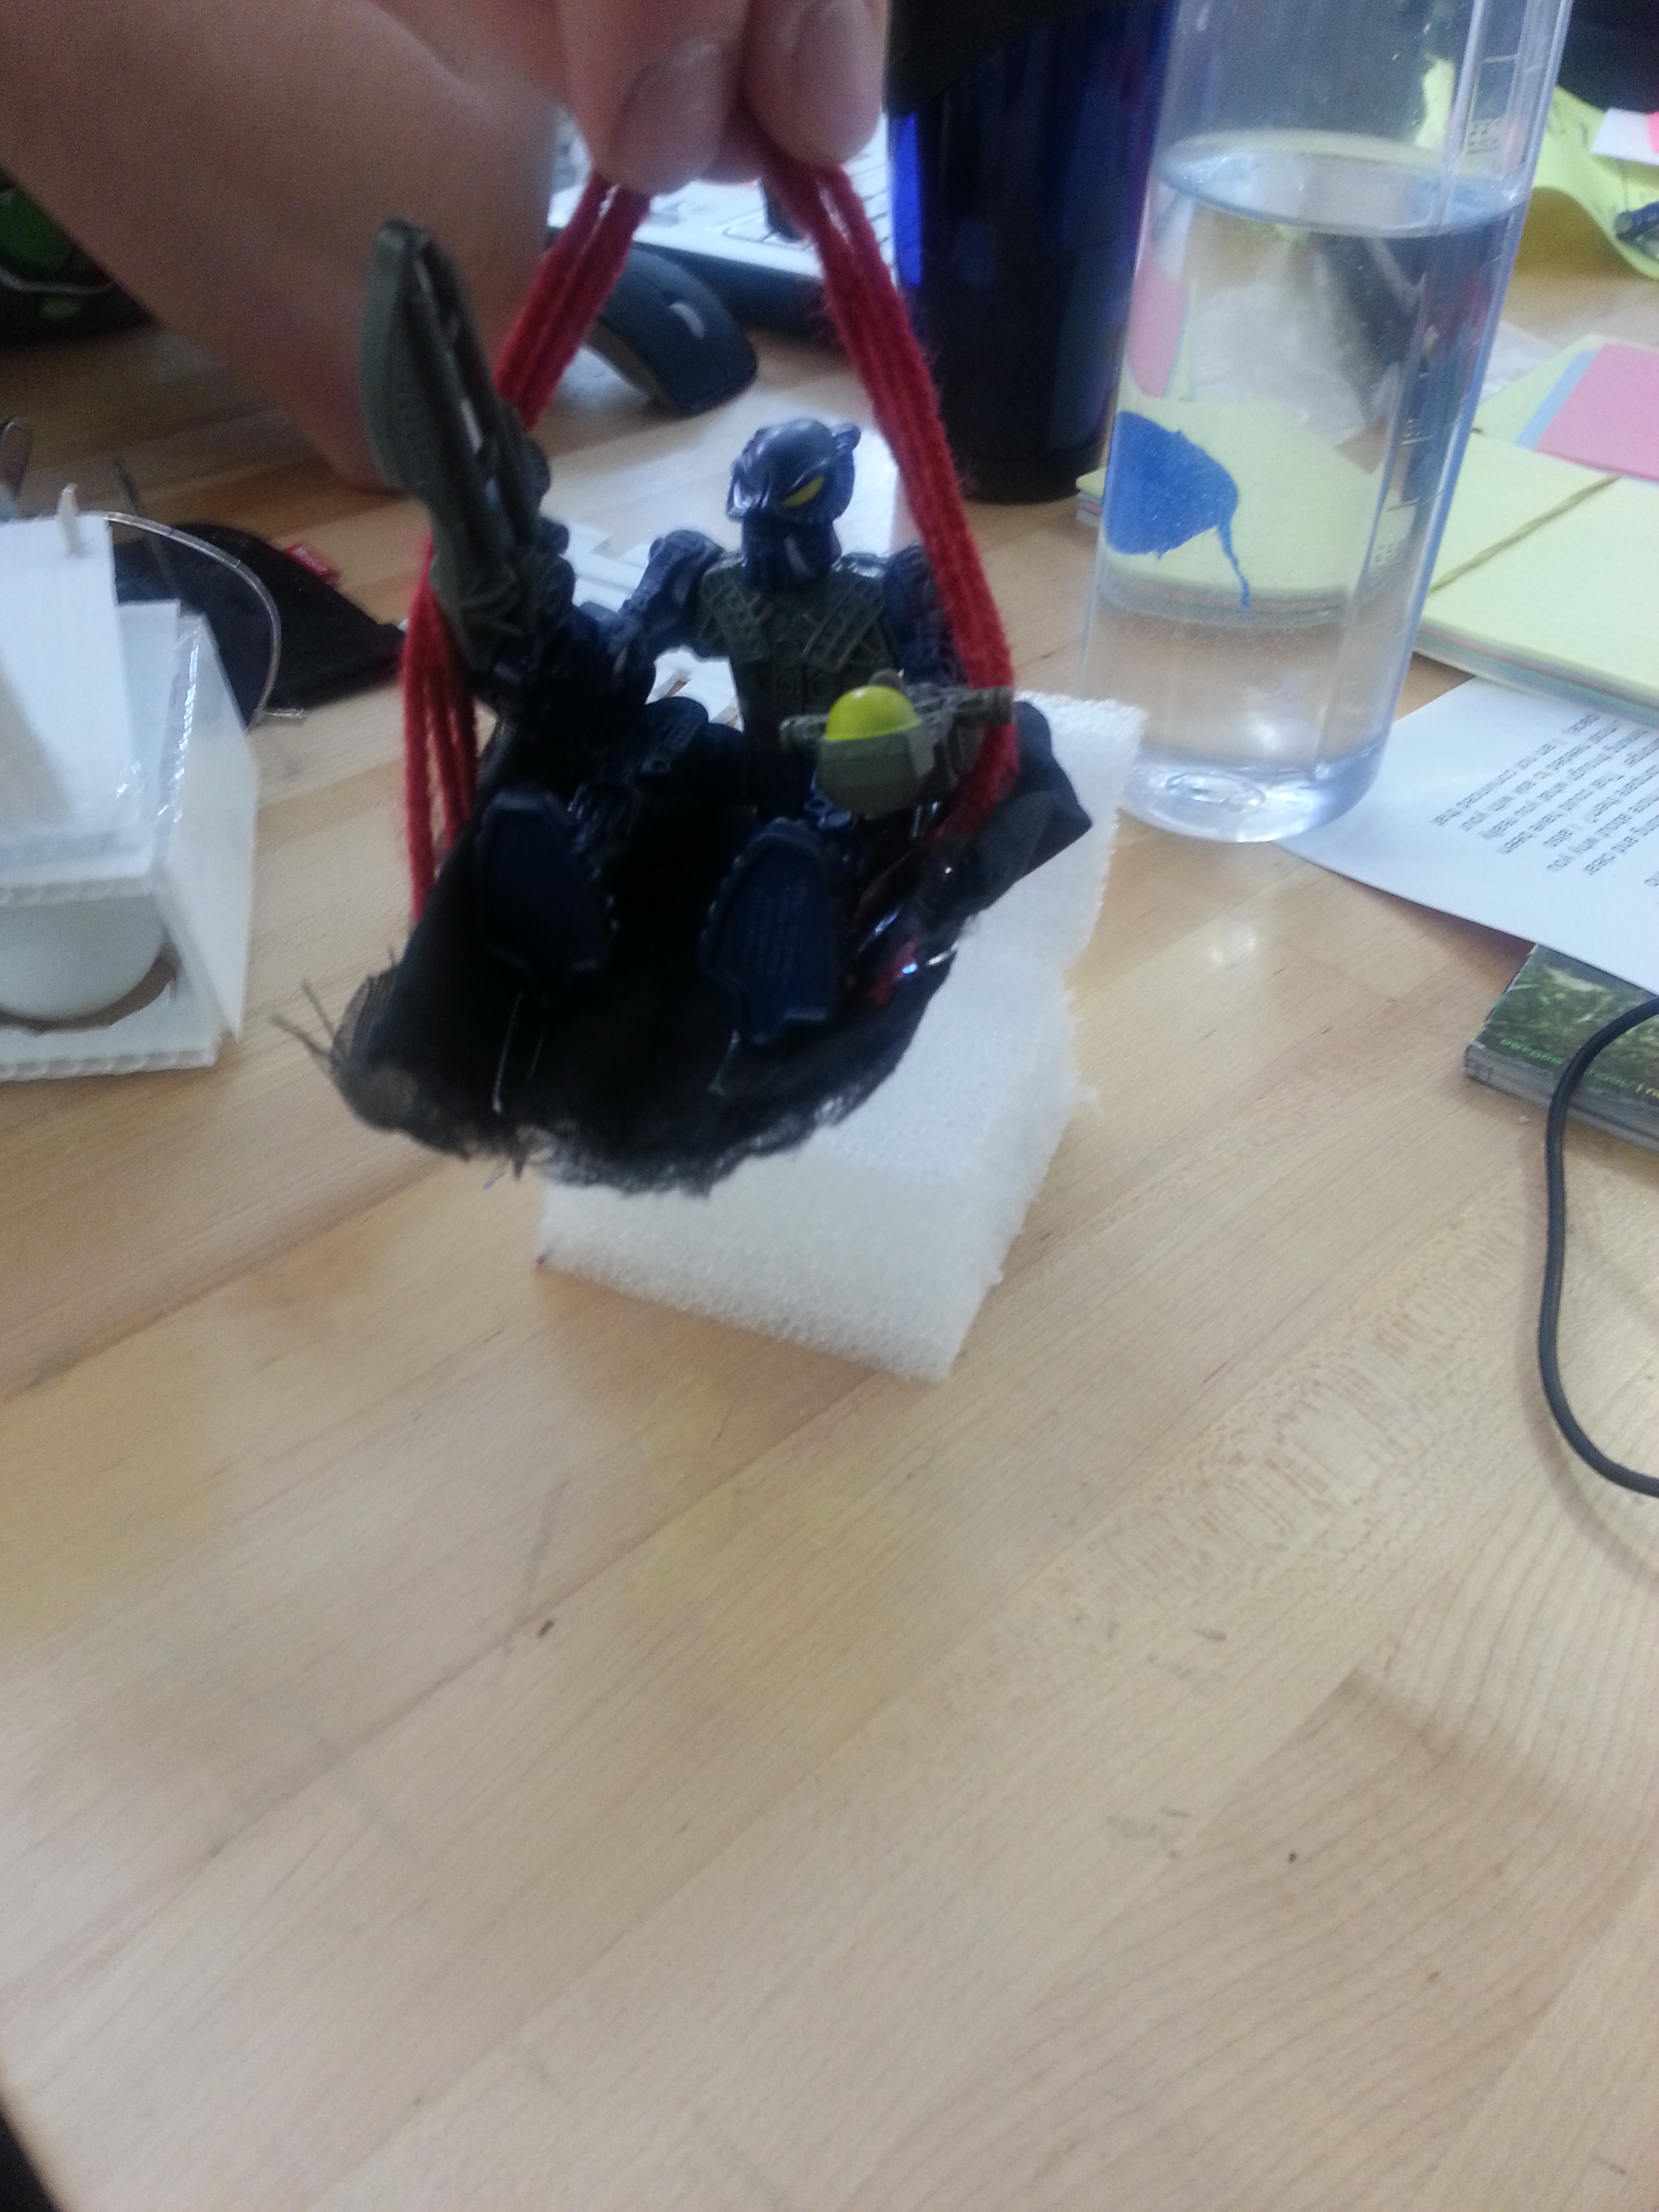
\includegraphics[width=7cm]{images/20140120_121827.jpg}
   \caption{Hammock transfer to enable people to go from the airport chair to their seat}
  \label{fig:20140120_121827}
\end{figure} 

	& The \textbf{comb} seat involves two separate pieces which have interlocking teeth; one can be lifted up, bringing the passenger with it, then installed on another chair
\begin{figure}[h]
  \centering
     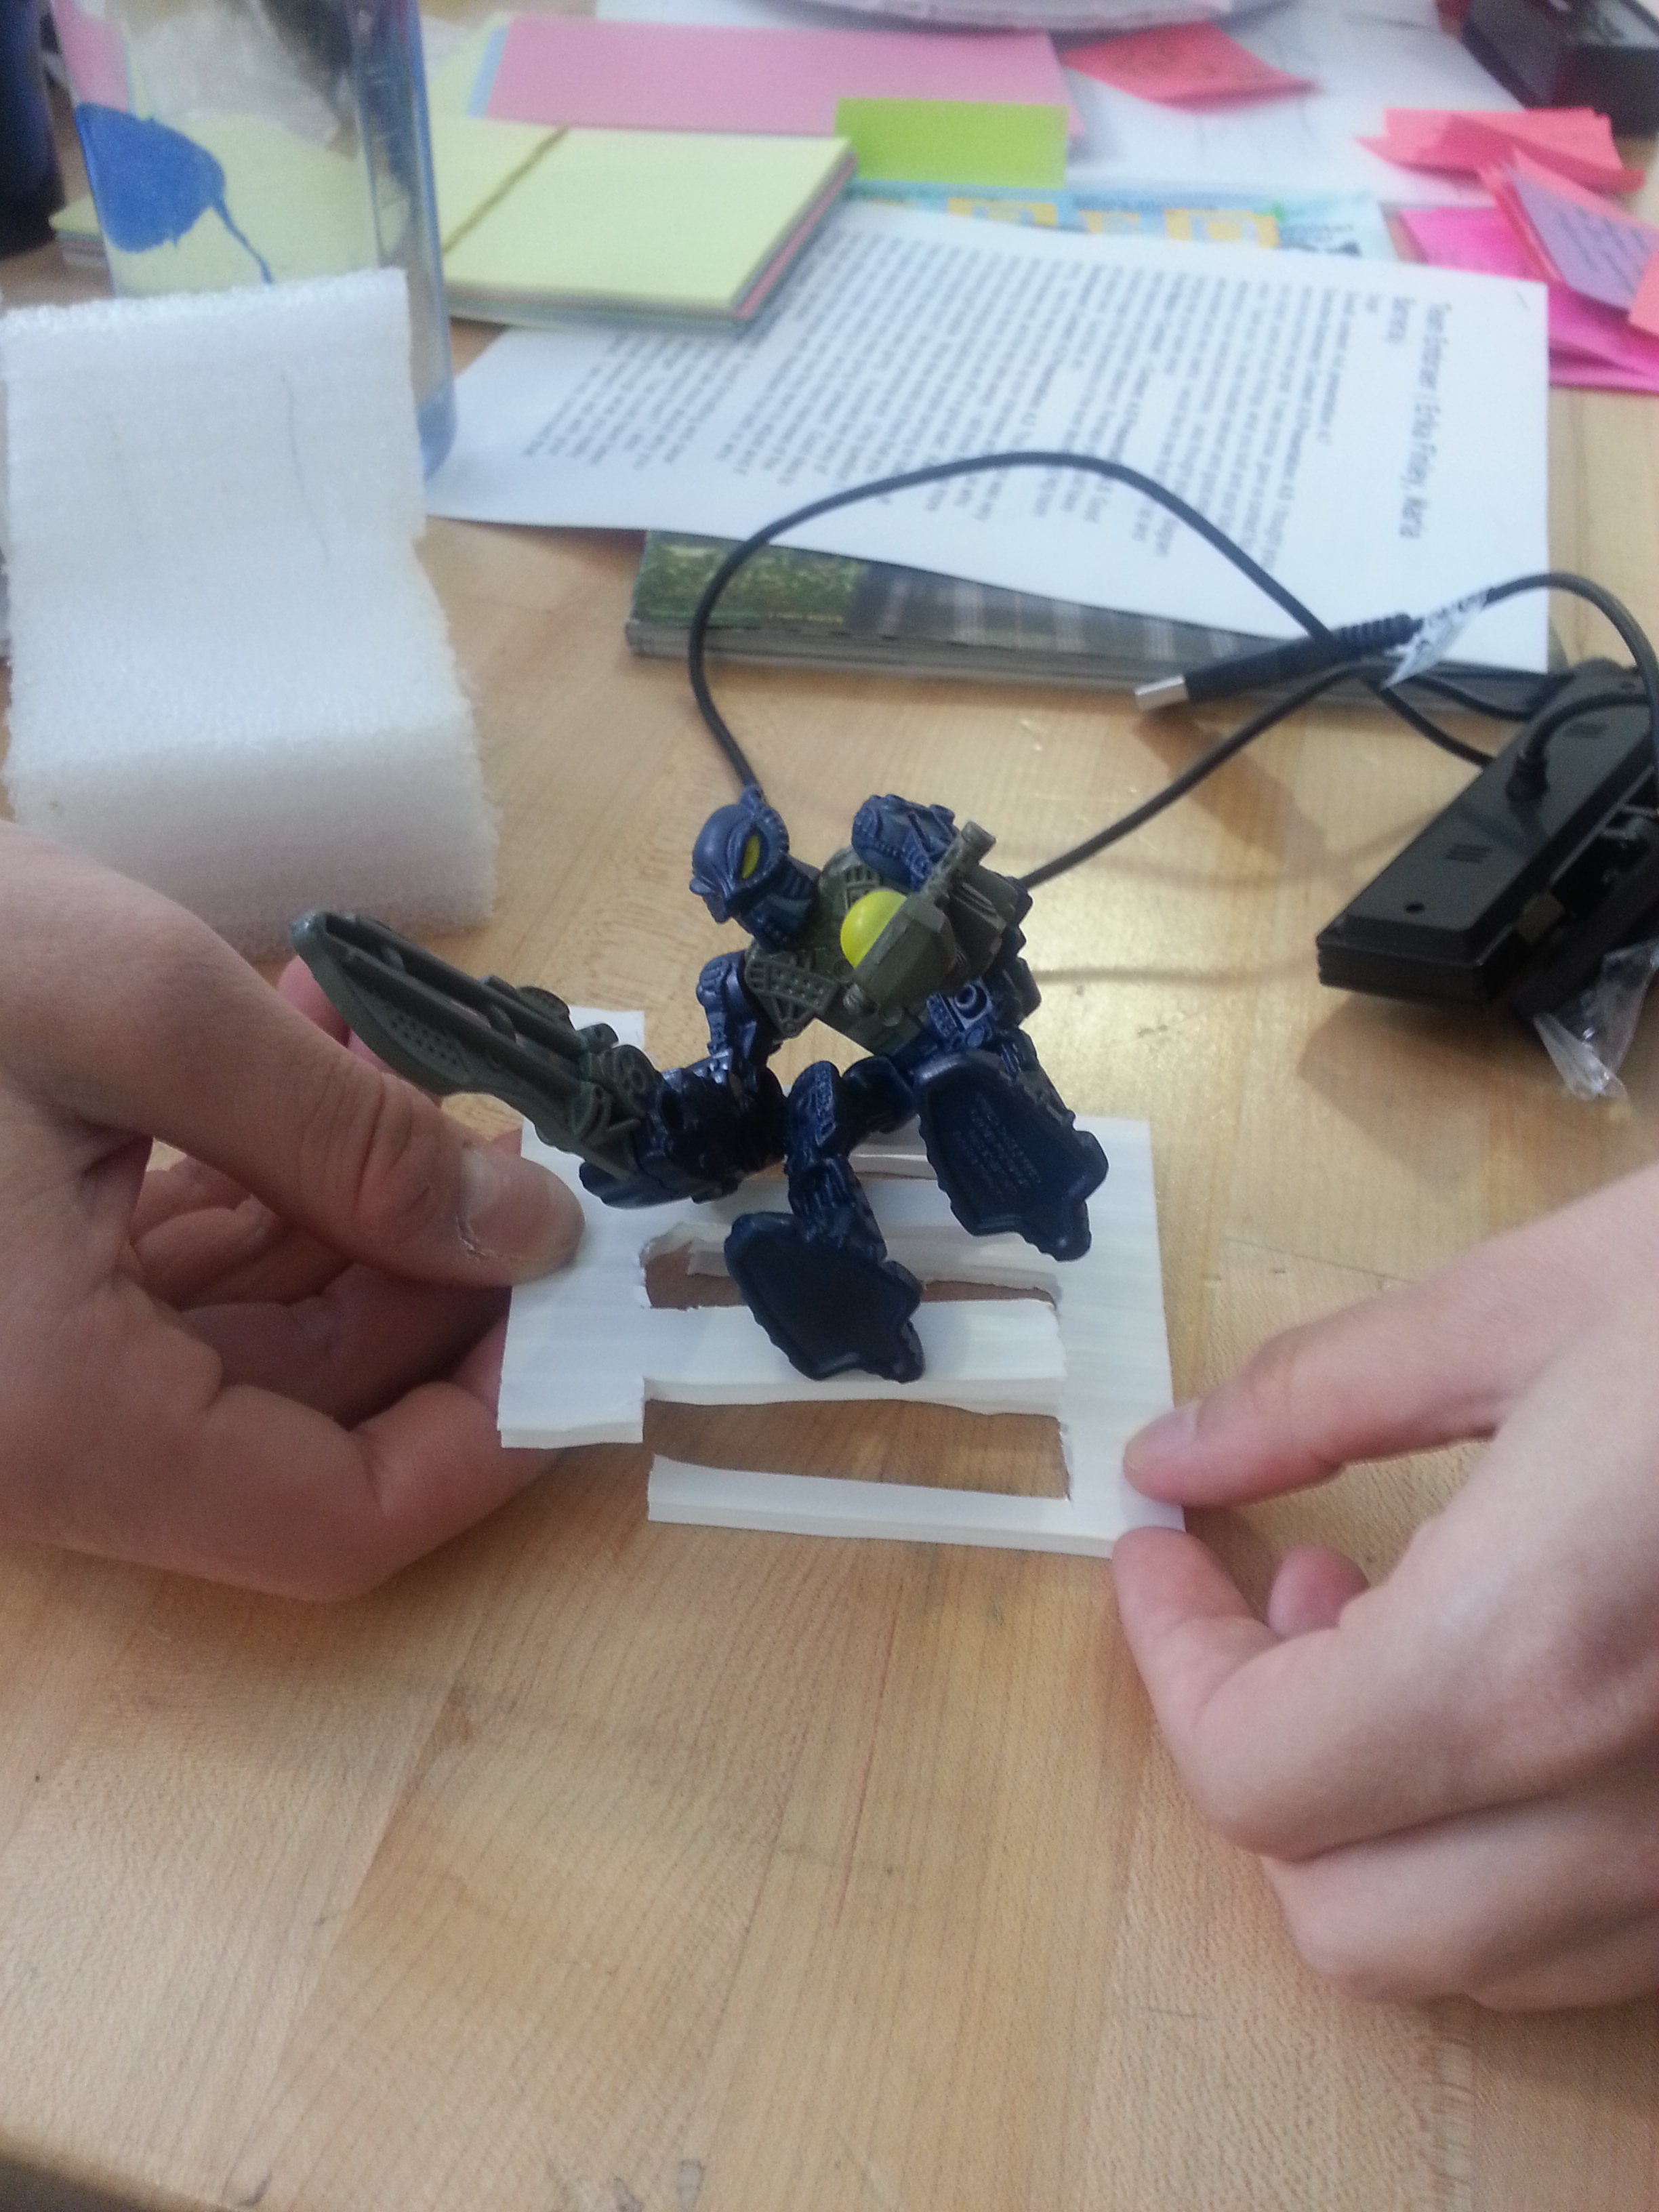
\includegraphics[width=7cm]{images/20140120_121849.jpg}
   \caption{Comb seats that would facilitate the transfer from the airport chair to the seat}
  \label{fig:20140120_121849}
\end{figure} 

\end{easylist}

& Once our user is seated, his seat will then be moved via the carousel/conveyor belt to its standard position as shown on the next drawing.

\begin{figure}[h]
  \centering
     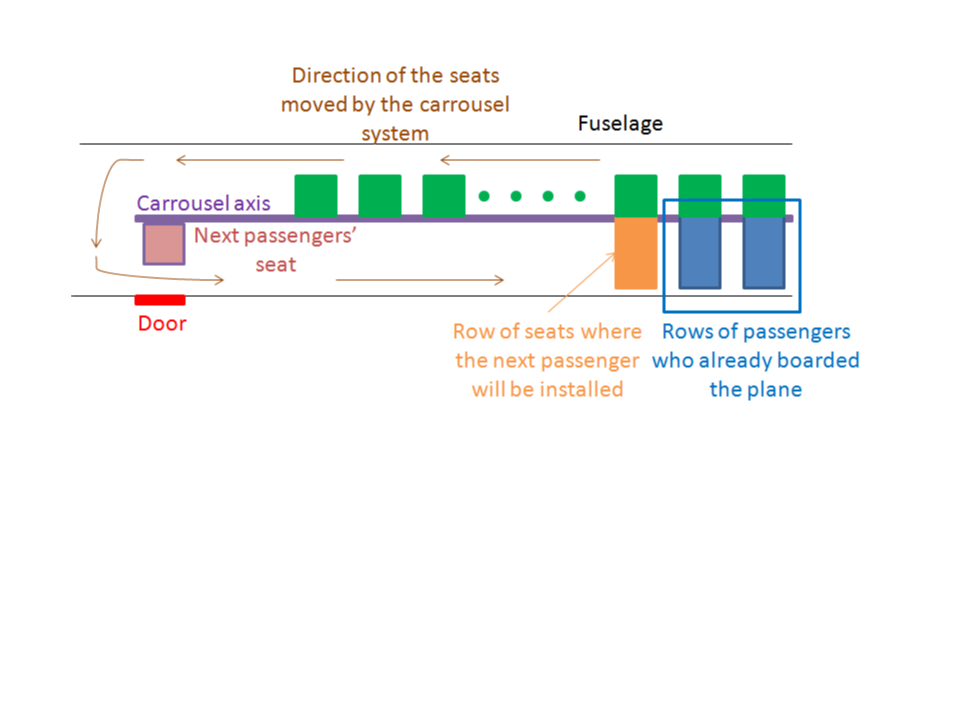
\includegraphics[width=7cm]{images/carousel_for_the_dummies.png}
   \caption{Carousel system conveying the seats from the entrance of the plane to their appropriate location}
  \label{fig:Carousel_system}
\end{figure} 
\end{easylist}

\subsection{Learnings}
The learnings for this iteration of darkhorse resulted from team discussions, user suggestions and feedback, observations of the user persona, and teaching team feedback. \\

\begin{easylist}[itemize]
	& The transfer mechanism to move the user into the airplane chair is still a problem that needs to be addressed. The user has to be able to make it from the waiting lounge to the airplane seat with the feelings of control, comfort and stability. 
	& The experience prototype of boarding did not include a mechanism to deal with luggage. The process of storing and carrying luggage needs to be addressed within the prototype to represent the entire experience. 
	& Communication is key to allow our users to feel comfort, safe, and stable within the new process. The process needs to be communicated effectively and sufficiently to allow for our users to have a better experience and to feel as if this process is better than the previous boarding process. 
	& Users want to be able to worry and stress less about getting to their seats and finding a place for their luggage. The new boarding process would allow the users to use the boarding time on a more enjoyable pastime. 
	& The users have to exert less effort with this boarding process because boarding is automated and does not require the need to locate their seats and maneuver the aisle. 
	& Our user was concerned with bumping into objects or other seats or hitting the wall during movement. The boarding process needs to be done in such a way that the users and passengers feel safe and secure with the movement and with process as a whole.  Lateral accelerations need to be considered to create a smooth ride and efficient boarding process. 
	& Sensors would need to be implemented into a functional prototype or a mechanical prototype to simulate the actual boarding process by having the interim stops to board new passengers.  Sensors would also need to be implemented into the process to prevent collisions or accidents in the case of a malfunction. 
\end{easylist}

\section{Dark Horse Version 3}
\subsection{Benchmarking}
During our user testing for our second version of the Dark Horse prototype, we realized carry-on luggage was a huge concern. Currently, luggage is stored in a very burdensome and unintuitive way and with version 3 we sought out to redesign the carry-on luggage experience. 
Our users have voiced their concerns about not being able to store/reach their luggage as well as the panic they feel when they are not aware of where their belongings are being stored. Our team looked at a couple of different designs out there that use the vertical space within the airplane in a different manner to accommodate both people and luggage in a more user friendly way. 

\begin{figure}[h]
  \centering
     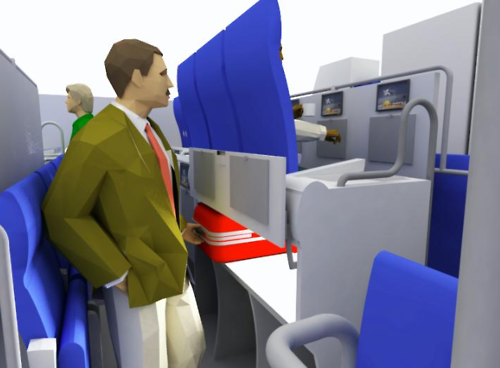
\includegraphics[width=7cm]{images/luggage_trays.png}
   \caption{Design that allows for easier luggage storage for all passengers \cite{blue_vertical}}
  \label{fig:luggage_trays.png}
\end{figure}  

The design shown in Figure \ref{fig:luggage_trays.png} displays a cabin layout where consecutive rows of seats are on different levels, allowing passengers to store their luggage behind their tray but under the seat of the person in front of them. This design puts luggage at the ideal height for both standing and sitting passengers as depicted by the image in Figure \ref{fig:correct_height.png}, a standard design rule for access and mobility.  

\begin{figure}[h]
  \centering
     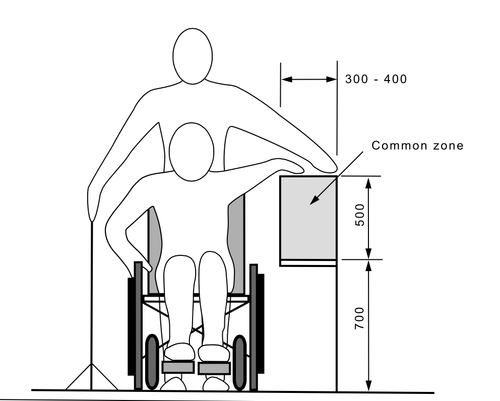
\includegraphics[width=7cm]{images/correct_height.png}
   \caption{Ideal height for reaching objects for both sitting and standing passengers. \cite{correct_height}}
  \label{fig:correct_height.png}
\end{figure} 

Another design solution we explored was actually having two seats on top of each other as shown in Figure \ref{fig:vertical_with_luggage.jpg}. This design opens up the area under the stairs for luggage storage, which could also include a passenger’s wheelchair, allowing for a less stressful flying experience for handicapped users. The bed next to the seat could also be used to provide passengers flying with toddlers with extra room to put them in so that they do not have to sit on their lap throughout the whole flight. 

\begin{figure}[h]
  \centering
     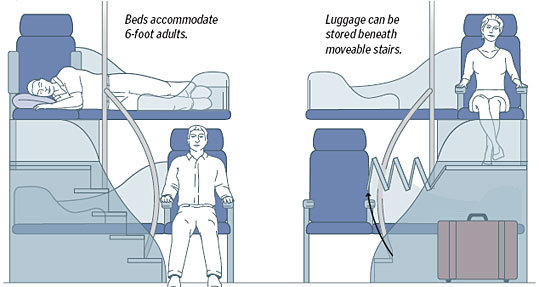
\includegraphics[width=7cm]{images/vertical_with_luggage.jpg}
   \caption{Vertical cabin configuration with luggage storage \cite{vertical_luggage}}% Source: http://www.boston.com/business/articles/2009/06/15/taking_airline_seat_configurations_vertical}
  \label{fig:vertical_with_luggage.jpg}
\end{figure} 
transfer

Another main concern for our user was the actual transfer process and how they would get from an aisle chair to their seat. We know that today people can use transfer boards, they can be carried by someone else or, if they are strong enough, they can transfer themselves. We found that there are some products on the market that could make the transfer experience better, such as the “harness” shown in Figure \ref{fig:harness.jpg} or the walker in Figure \ref{fig:walker.jpg}. We believed that the walker would be an interesting solution if we were able to add mechanisms  that would lower the bar supporting the person’s weight to get it closer to the seat and that would swing the blue supports open such that the person would come in contact with the chair. Eventually, we actually decided to widen the airplane aisle and get rid of the transfer all together. 

\begin{figure}[h]
  \centering
     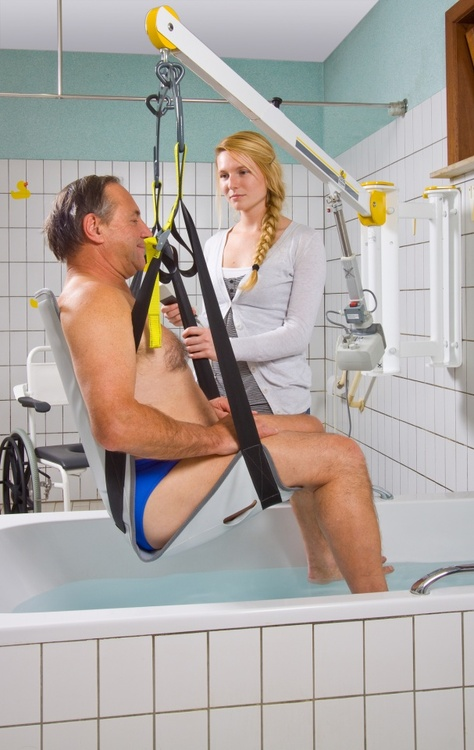
\includegraphics[width=7cm]{images/harness.jpg}
   \caption{Harness used to get disabled out of the bath. \cite{harness}}% Source: http://www.handimove.com/en/products/bath-seat-pvc/}
  \label{fig:harness.jpg}
\end{figure} 
transfer

\begin{figure}[h]
  \centering
     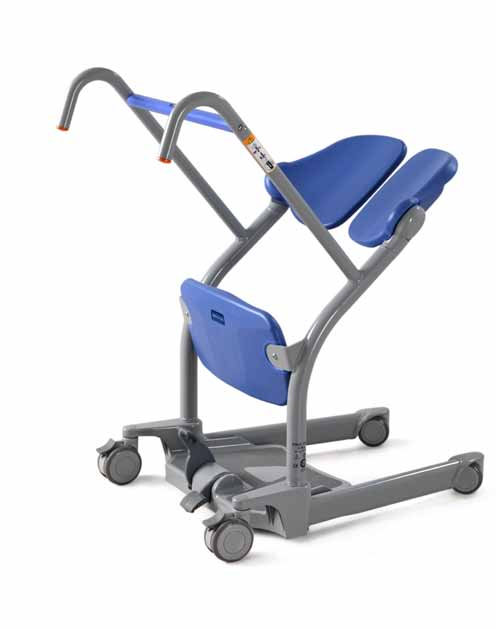
\includegraphics[width=7cm]{images/walker.jpg}
   \caption{Walker that could be adapted to become a better aisle chair. \cite{walker}}% Source: http://mobilityexpress.com/Sara-Stedy-Seated-Transfer-Device_1154.htm}
  \label{fig:walker.jpg}
\end{figure} 
transfer

\subsection{Description}
Currently, people with reduced mobility have to first transfer from their own wheelchair to the aisle wheelchair which is uncomfortable and narrow. Once boarding starts, the user is brought to his/her seat by a flight attendant or an airline employee and is then transferred to his/her seat. This process is long, it puts people with reduced mobility apart by making them different and it deprives them from their independence because the aisle wheelchair must be manoeuvered by a flight attendant. Therefore, since the boarding process is such a pain point for our users we decided to work on it to improve their experience and give them more independence.

During the boarding process the two steps that are critical for our users are :

 \begin{easylist}[itemize]

& First, the access to their seats. Our team thought that if we could enable people with reduced mobility to enter the aircraft with their own wheelchair and then give them the possibility to transfer themselves from their wheelchair to their seat without someone else helping them it would considerably improve their experience.

& Second, the luggage storage. People with reduced mobility frequently cannot access the luggage compartment because it is too high, so our team thought that if we could imagine a system that makes the luggage compartment go up and down by just pressing a button it would also contribute to make the flight experience better for people with reduced mobility.

\end{easylist}

1. Helping our user access his/her seat :

Our objective was to enable passengers to enter the aircraft with their own wheelchair and to do so we had to figure out a way to make the aisle wider. Initially we did not want to take into account the constraint of keeping the number of seats in the aircraft the same so we imagined a new cabin layout for boarding. The idea was to have the aisle seats on rails so that they could be moved and lined up with the window seats as shown in Figure \ref{fig:first_new_cabin_layout} . 

\begin{figure}[h]
  \centering
     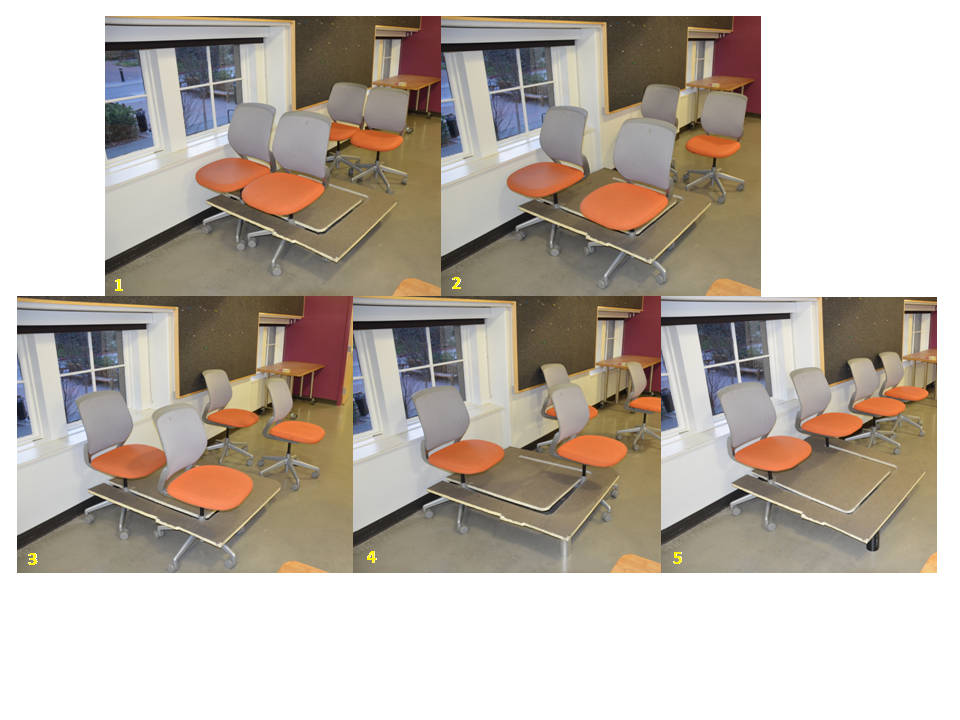
\includegraphics[width=7cm]{images/first_new_cabin_layout.png}
   \caption{Our first new cabin layout for boarding the plane}
  \label{fig:first_new_cabin_layout}
\end{figure} 

With this system all the seats would be lined up on each side of the plane and the aisle during the boarding process would then be three times bigger than in flight, allowing people with reduced mobility to enter the aircraft with their own wheelchair which is on average 30’’ wide, as shown in Figure \ref{fig:wheelchair_dimensions} .

\begin{figure}[h]
  \centering
     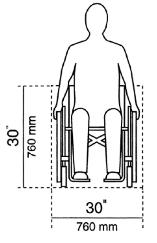
\includegraphics[width=7cm]{images/wheelchair_dimensions.png}
   \caption{Standard wheelchair dimensions}
  \label{fig:wheelchair_dimensions}
\end{figure}

But we realized that with this system it was impossible to keep the total number of passengers on board the aircraft the same because the proposed boarding layout requires too much space per seat. 

Therefore, we thought of a second cabin layout for the boarding process which also makes the aisle wider but in a more reasonable way. We looked at the dimensions of a standard Embraer plane (Figure \ref{fig:embraer_plane} ) and found out that if we were able to angle the rows by 46.2° (see Figure \ref{fig:angled_seats}) from their current position we could make the aisle wide enough (42.87’’) to enable our passengers to reach their seats in their own wheelchair while keeping the total number of seats the same.

\begin{figure}[h]
  \centering
     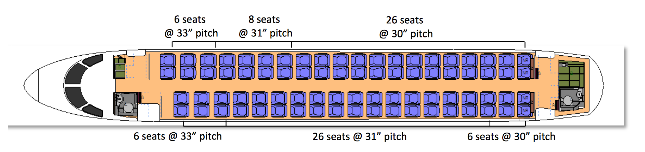
\includegraphics[width=7cm]{images/embraer_plane.png}
   \caption{Standard Embraer plane cabin layout}
  \label{fig:embraer_plane}
\end{figure}

Our concept was to initially have all of the rows of the plane linked to a mechanism that would rotate the seats before the boarding process, making a wider aisle for passengers. Passengers with reduced mobility who have reached their seats with their own wheelchair would be able to transfer to their plane seats. If they are strong enough they may be able to transfer themselves without requesting flight attendants assistance, but if they need help we imagined that they could use one of the transfer mechanisms mentioned in the benchmarking section.
\begin{figure}[h]
  \centering
     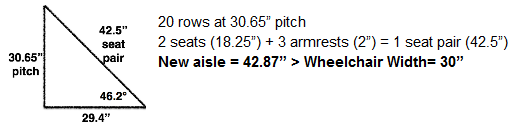
\includegraphics[width=7cm]{images/angled_seats.png}
   \caption{New cabin layout with angled seats for boarding}
  \label{fig:angled_seats}
\end{figure}

Once the passengers are all seated (potentially while the aircraft is taxiing towards the runway) the seats would go back to the standard non angled cabin configuration for take off and would remain in that state for the duration of the flight. When the plane stops at the gate and is ready for passengers to disembark, the seats would be angled again and flight attendants would bring passengers with reduced mobility their own wheelchair so that they would be able to leave the plane on their own. 

2. Helping our user accessing the luggage compartment :

We found out that accessing the seat is not the only problem disabled people are confronted with: they also have a big issue when they want to store their personal items in the luggage compartment. In order to fix this, our team designed a luggage compartment that can go up and down on demand, controlled by our user pressing a button (Figure \ref{fig:embraer_plane}).

\begin{figure}[h]
  \centering
     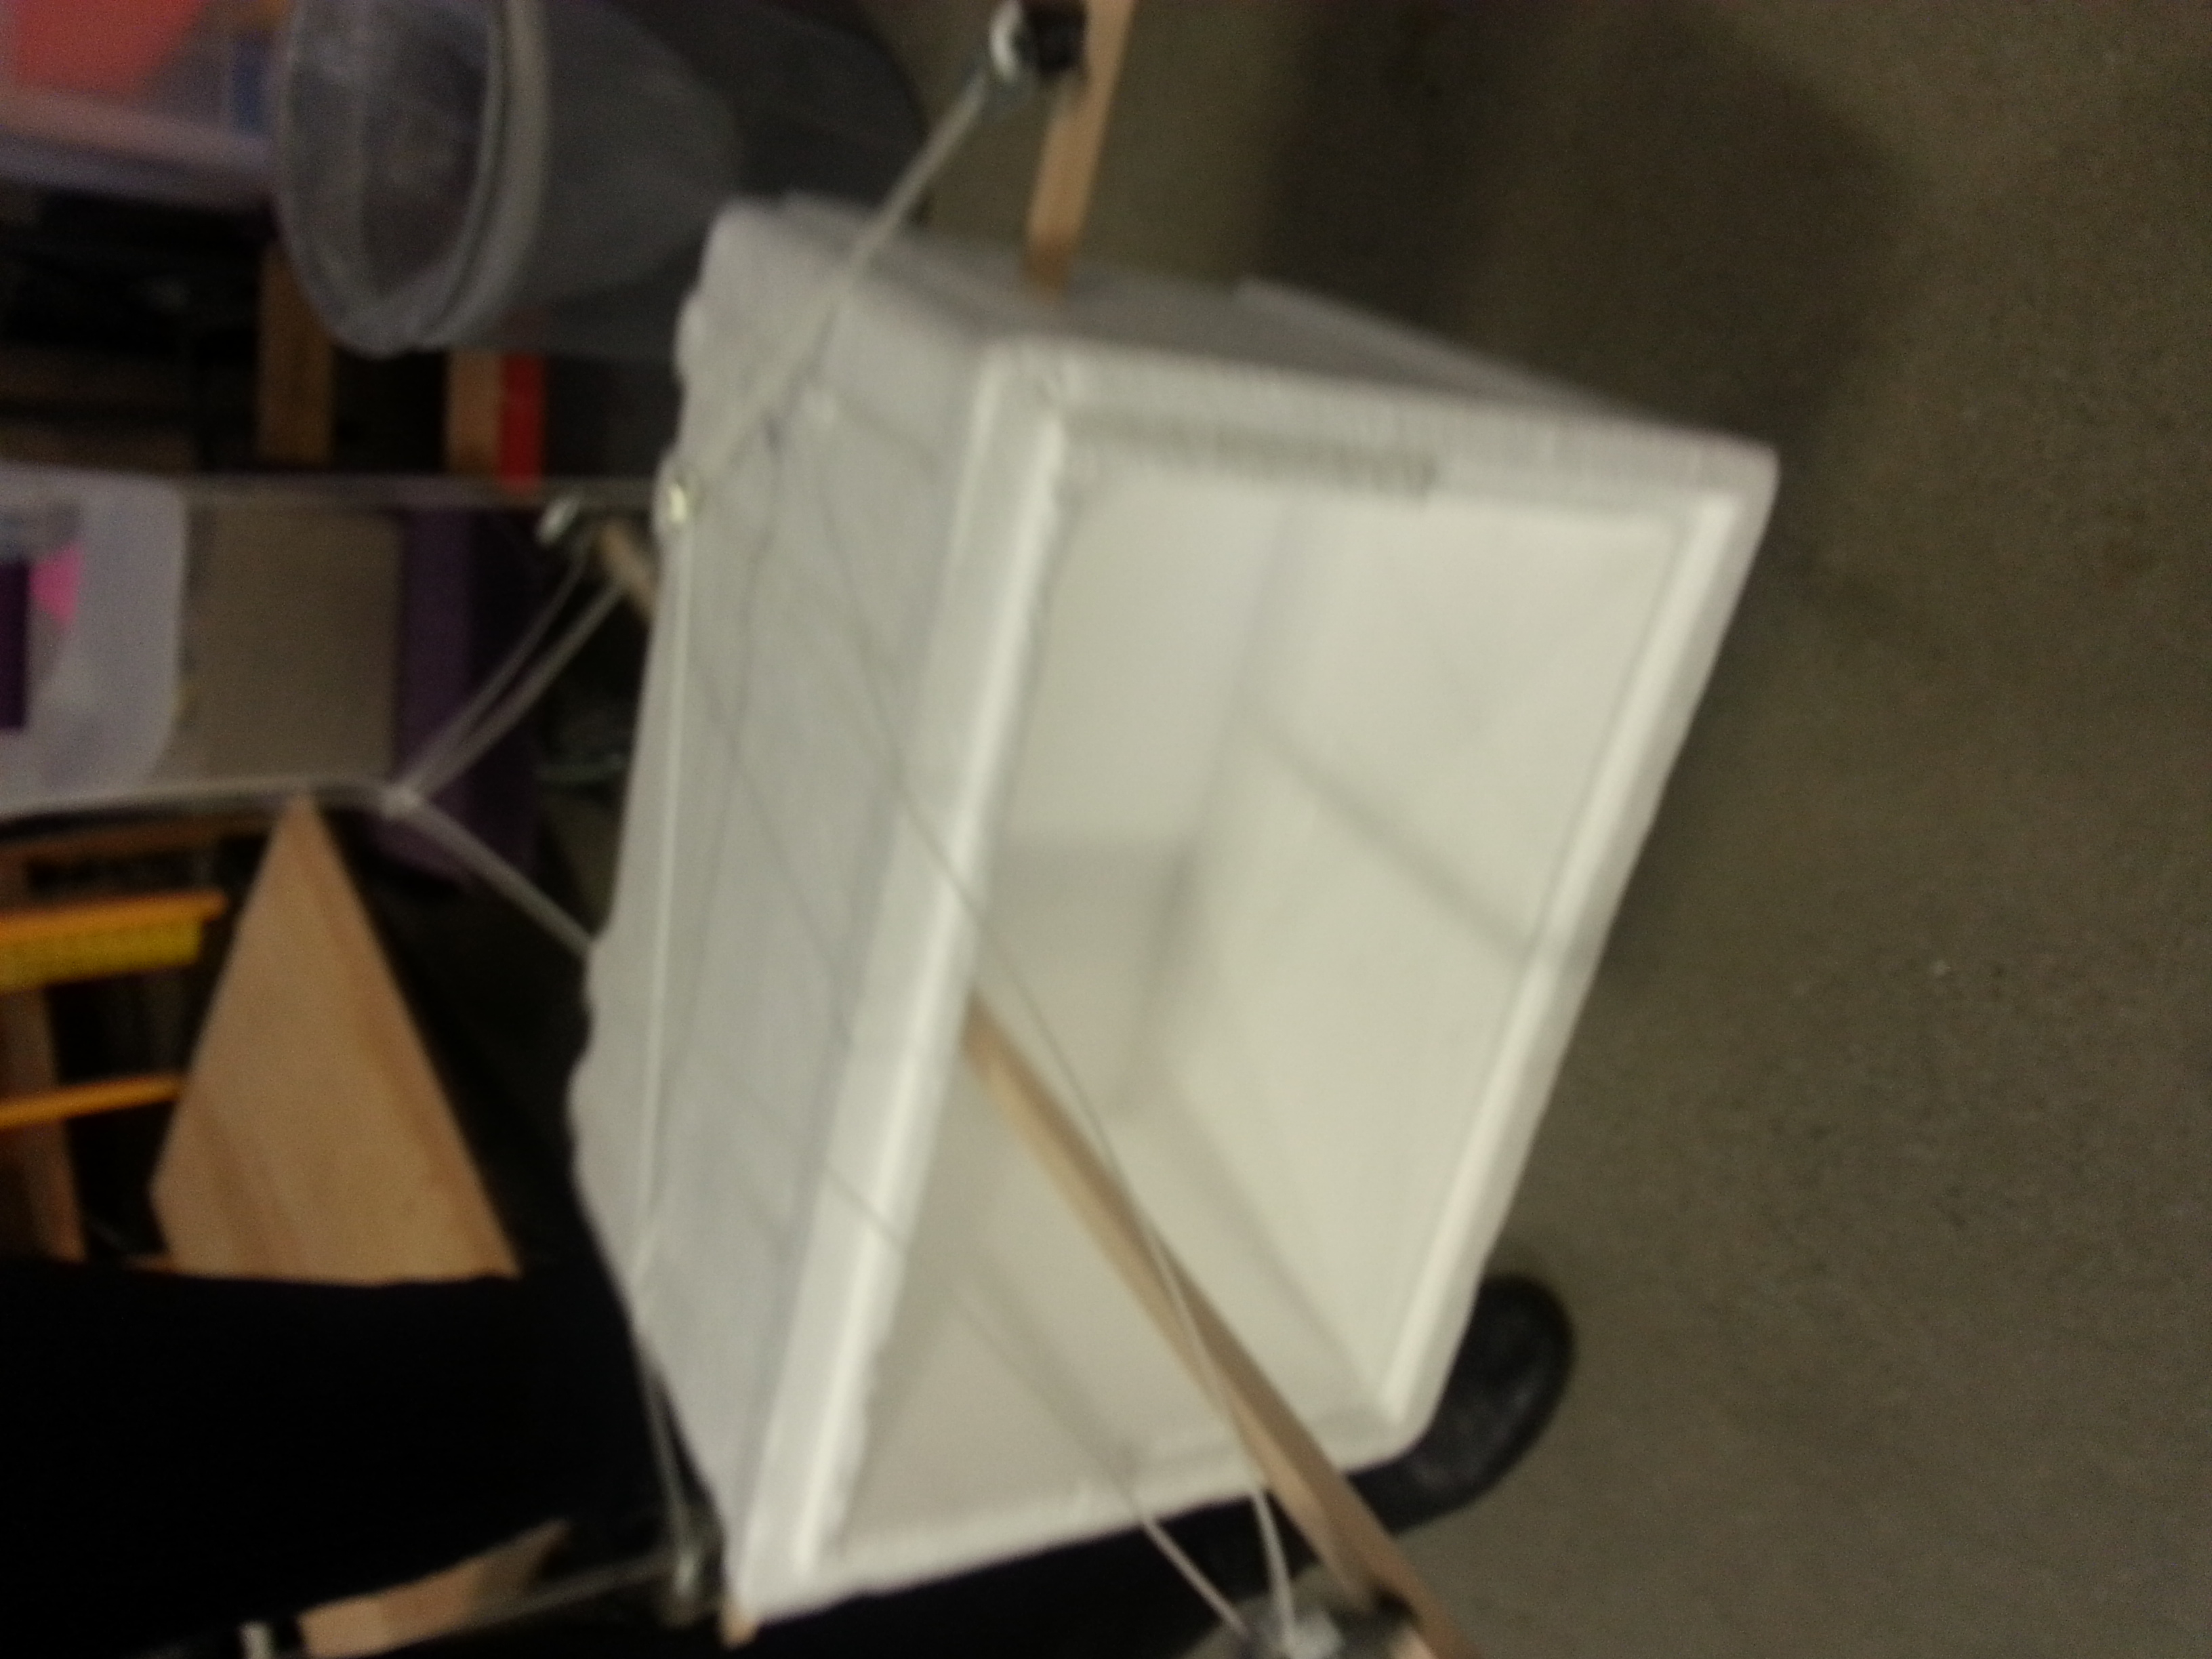
\includegraphics[width=7cm]{images/20140130_170818.jpg}
   \caption{Our luggage compartment which is accessible on demand by pressing a button}
  \label{fig:our_luggage_compartment}
\end{figure}

In order to build this system we designed a mechanism made of rope and pulleys that is inspired from systems used to stabilize cameras that are mounted on drones and model aircraft. While piloting the system that causes the camera to move, the device has to remain stable. This mechanism avoids the creation of moments that could cause the ropes to tangle and knot. For our system we wanted to have a luggage compartment that does not experience torques and that can come up and down in the most smooth and stable way.

\subsection{Learnings}
Several classmates and peers were users for this prototype and provided the majority of our learnings.  However, some of the learnings came directly from team observations during user testing. The learnings are divided into the reconfiguration and the luggage. 

\textbf{Reconfiguration:}
\begin{easylist}[itemize]
	& Our testing revealed that the users were concerned about what would happen to their feet during the transformation of angled seating to the regular configuration and vice versa.  Some users suggested the addition of a footrest.  But where would the ideal location be? This revelation is very important to our target users because some of them do not have the ability to move their legs out of the way or to move with the chair.  This would also mean they would have to manually put their feet on a footrest, and the ideal position of the footrest would need to be designed to help the target users have a better experience.
	& A single, continuous rotation mechanism would be better than multiple discrete for all passengers.  The users commented that the mechanism should be similar to the movement of a car seat because it is slow enough and does not cause a great amount of force and acceleration to be placed on the passenger. In addition, the window seat experienced less movement or felt like it experienced less movement than the aisle seat.  This is important due to the benchmarking findings of last quarter that showed that the target users preferred the window seat over the aisle seat. 
	& Passengers would be able to board faster due to a wider aisle that allows for easier maneuvering of the cabin space.  The wider aisle would allow for a double line of traffic to head down the aisle instead of one line. 
	& The wider aisle would allow for a wheelchair to be able to maneuver down the aisle to the seat.  The wheelchair would have tolerances on both sides as it moves down the aisle to allow for a comfortable fit.  It would be easier for a mobility challenged passenger to get into the aisle seat but to access the window a handle may be needed. 
	& The legroom is the limiting factor with the reconfiguration.  When the seats are in the angled arrangement, the window seats have less legroom than in the normal configuration.  The angle of the seats would need to be reconfigured to allow for a smaller angle with more legroom but still create a wider aisle with plenty of tolerance for a wheelchair. However, it was noted that it is easier to board and deboard with angled seats.  Thus, angled seats would be the preferred configuration for boarding and disembarking from the plane. 
	& It may be possible to achieve the desired effect by only rotating several of the aisles, allowing increased access to those seats specifically.

\end{easylist}

\textbf{Luggage:}
\begin{easylist}[itemize]
	& The luggage bin needs to move with the seats into the angled configurations. With the bins situated parallel to the normal cabin configuration when the seats are angled, it is difficult to load the luggage into the bin without awkward movements. 
	& The luggage bin should be lowered to arm level instead of head or face level.  Users felt claustrophobic when the bin was at head level due to the reduction in vision. The bin was in the line of sight which made it uncomfortable and a very closed-off space.  
	& The bin should have a door and have a slightly steeper angle or have a lip. Luggage moves during flight due to turbulence and shifting due flight. This would prevent luggage falling out on the passengers or items being broken. 
	& A more rigid lowering mechanism needs to be used instead of the string and rope mechanism that was used during prototyping.  Users did not feel that the bin was stable and looked scared as it was lowered down.  They feared the bin might move during lowering, raising, or turbulence causing it to hit them or bring their belongings.  
	& More research for optimal lowering position needs to be conducted.  The position that we prototyped did not receive good feedback from the users.  Therefore, several iterations need to be performed to see what would be best for our target users and other passengers
	& Most of the users wanted to store luggage before they sat in their seat.  The orientation of the bin and the height of the bin makes this a very awkward and uncomfortable task.  When the users sat with their luggage, they felt that they were crowded and did not know what to do with the luggage until the bin was available.  The mechanism to raise and lower the bin needs to be fast and stable to allow for ease of access to the seat and aisle depending on the activity.
\end{easylist}

\section{Funky Prototype}


\subsection{Benchmarking}
\subsection{Description of the prototype}
\subsection{Learnings}
\section{Going Back to The Need}
Following the wrap up of our funky prototype, the Stanford team decided to take a step back to figure out if we were truly solving the burning need. We analyzed all of our prototypes up to this point and saw an overarching theme we were trying to address: giving our users their independence back. With independence as our umbrella, our team looked at the whole flying experience piece by piece, with the purpose of identifying the points at which independence truly breaks down. 

We went back to our needfinding from fall quarter, sent surveys to both old and new contacts and carried out more interviews. All of these allowed us to confirm that mobility within the cabin is, in fact, a huge issue and that the team at USP should continue working on the transfer system. However, this new information also brought to light a burning need we had initially discarded fall quarter - wheelchair storage. Furthermore, both of these needs stem from the same procedure the wheelchair user is forced to go through: that of giving up his/her wheelchair. 

\subsection{The Problem}

Imagine you are a wheelchair user. You arrive at your gate, ready to board your plane, and are told you need to hand over your wheelchair for storage in the cargo hold. At this point, you ask yourself two questions: 
\begin{enumerate}
	\item How will you move now that you don't have your mobility device? 
	\item Will your mobility device come back safe and sound at your destination?
\end{enumerate}
The following sections will detail the user quotes and research that led us to choosing both of these directions.  
\\

\textbf{Mobility In the Cabin}

In order to comfirm the need for improving mobility inside the cabin, we asked our contacts to fill out a survey that would give us a better idea of what exactly would be the most helpful for them. The full survey responses can be found in Appendix \ref{"SOMEONE FILL THIS IN? IM NOT SURE HOW THE APPENDIX WORKS, can you add pdfs to it?"} 
When asked about the prospect of having an ``on demand"  powered aisle chair, users were keen on the independence it would provide as it would allow them to ``board the plane at [their] own pace and go to the restroom when [they] please." One of our respondants stated that such a device would allow them to ``feel like a passenger for a change and not a sack of coffee beans". This quote clearly depicts the struggle users currently go through when they give up their mobility device and with it, their independence.

Our team assumed that having such a chair would be a great improvement to the experience yet we could not figure out if the chair had to be completely autonomous and show up on demand or if a flight attendant could bring it to the user. What we found is that users would much rather have automated systems than feel the guilt of inconveniencing someone else to do something for them, even if it only meant they had to bring them a chair just like they bring any passenger a drink or snack. 

Finally, we decided to delve deeper into the transfer process. One of our interviewees, Scott Rains, had told us about a friend who was injured as he was being transferred from the aisle chair into his airplane seat. The airport personnel did not lift him up high enough and his bottom was hit against the armrest. Given that wheelchair users have thinner and more sensitive skin in this area, this caused him lots of pain and even resulted in 3 weeks spent at the hospital. While injuries are not the norm, it is a very dehumanizing and undignified experience, just as Esther Appleyard-Fox states in her tweet in Figure \ref{fig:MobilityTweet.png}. 


\begin{figure}[h]
  \centering
     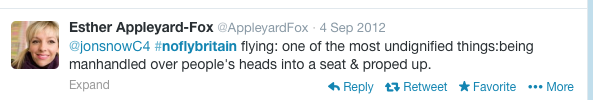
\includegraphics[width=9cm]{images/MobilityTweet.png}
   \caption{Tweet from Esther Appleyard-Fox explaining how she feels when she is transferred when she flies. }
  \label{fig:MobilityTweet.png}
\end{figure}


\textbf{Wheelchair Storage}

As we were looking for more data to substantiate our claim that mobility in the cabin was, in fact, the problem to solve, we stumbled upon another huge problem. During our interview with Aubrie Lee, a student in Product Design at Stanford University who is also a wheelchair user, she mentioned that while mobility inside the cabin is a problem, it is such a short part of her experience that she hardly remembers it as being painful. Part of this is due to the fact that when she travels with her dad he carries her down the aisle which I am sure can be more comforting than dehumanizing. However, she emphasized that``the most emotional part of [her] flying experience is having to give up [her] chair and waiting for them to give it back." For her, giving up her chair is ``a huge source of anxiety - as soon as it is out of [her] sight, [she doesn't] know where it is", whether it is going to come back to her unharmed or whether it is even going to make it to her destination. 

A study by Trailblazers \cite{trailblazers}, a group of disabled campaigners across the UK who tackle social issues affecting young disabled people, shows that 60\% of wheelchairs are damaged when traveling with an airline. As David Gillon says in Figure \ref{fig:60percenttweet.png} below, we must do better. 


\begin{figure}[h]
  \centering
     
\includegraphics[width=9cm]{images/60percenttweet.png}
   \caption{Tweet from David Gillon on Trailblazers study that shows 60\% of wheelchairs are broken in airline travel. }
  \label{fig:60percenttweet.png}
\end{figure}

\begin{figure}[h]
  \centering
     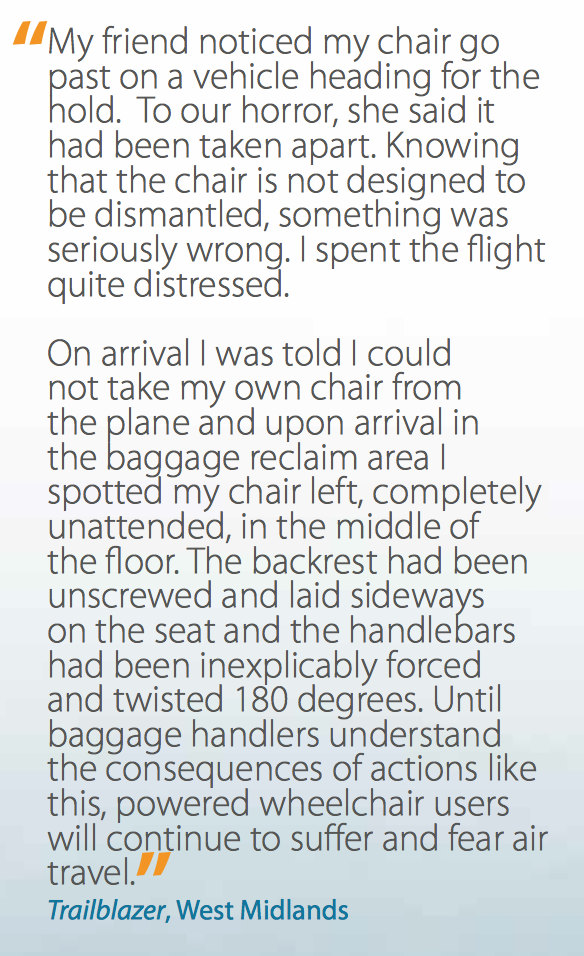
\includegraphics[width=5cm]{images/wheelchairstory.png}
   \caption{Anecdote from a Trailblazer that had her wheelchair broken during flight. \cite{trailblazers}}
  \label{fig:wheelchairstory.png}
\end{figure}

Stories like the one shown in Figure \ref{fig:wheelchairstory.png} are not uncommon, with wheelchairs ending up like the one in Figure \ref{fig:brokenwheelchair.png} due to airport personnel attempting to dismantle it or from the wheelchair moving around in the cargo hold. 


\begin{figure}[h]
  \centering
     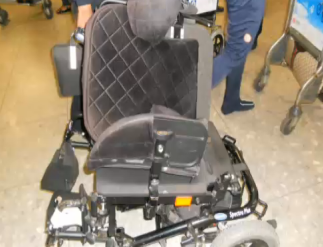
\includegraphics[width=7cm]{images/brokenwheelchair.png}
   \caption{Picture of a broken wheelchair after a flight. \cite{broken_wheelchair}}
  \label{fig:brokenwheelchair.png}
\end{figure}

There are also instances of the wheelchair not even making it to the destination, just like what happened to Josie shown in Figure \ref{fig:leftwheelchair.png}. 

\begin{figure}[h]
  \centering
     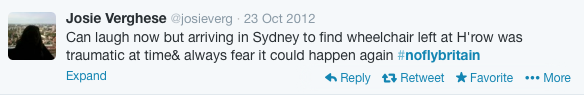
\includegraphics[width=9cm]{images/leftwheelchair.png}
   \caption{Tweet from Josie Verguese about her experience when her wheelchair did not make it to her destination.}
  \label{fig:leftwheelchair.png}
\end{figure}

Now to put this into perspective, imagine that you are a wheelchair user and you rely on your mobility device for you independence. This wheelchair isn't just an object, it is your legs, your independence, part of who are you. As Aubrie stated ``it is in limbo between being a physical object and half of me." Now imagine that after your flight, you no longer have the ability to move. This is a HUGE problem for our users, one we need to focus on. \\
\\

 Through  the user interviews, surveys and research depicted above, we have proven to ourselves, our advisors and our users that these are the 2 most compelling needs we need to address for our users. 


\section{Functional Prototype}
Winter quarter was brought to a finish with the third and final prototyping mission, Functional.  Unlike Funk-tional, the functional mission desires the creation of a working prototype with system integrations using materials that could be possible in the final vision, which means no duct tape or foam core. The functional mission leads the team into the spring quarter by aiding in the finalization of the vision and creating direction.  To find the direction and the vision, more needfinding might have to take place to confirm a need and verify the thinking and decisions of the team. Functional mission serves as the stepping point from iterative prototyping missions to the iterative final product mission.

\subsubsection{Benchmarking}
Before prototyping our first wheelchair storage device we did a larger search both for existing wheelchair storage and protection devices as well as methods for securing wheelchairs. We found several relevant patents for protection devices as well as regulations for securement, relating primarily to bus travel.

**********


\subsection{Wheelchair Storage Description}

As our last round of needfinding and research had brought to light the importance of wheelchair storage, the Stanford team decided to prototype the first version of what a wheelchair storage device could look like. This first prototype, shown in 
Figure \ref{fig:wheelchairprototype1.png}, focused on having a rigid floor to distribute wheelchair as well as a place to attach the hooks that would secure the wheelchair down. It had rigid walls that would serve to protect the wheelchair (as if it were a box) that were also hinged at the side so they could be moved out of the way of the person tying down the wheelchair. We opted to use the straps and hooks mechanism that people are already familiar with from buses and trains to create a sense of trust an security. 

\begin{figure}[h]
  \centering
     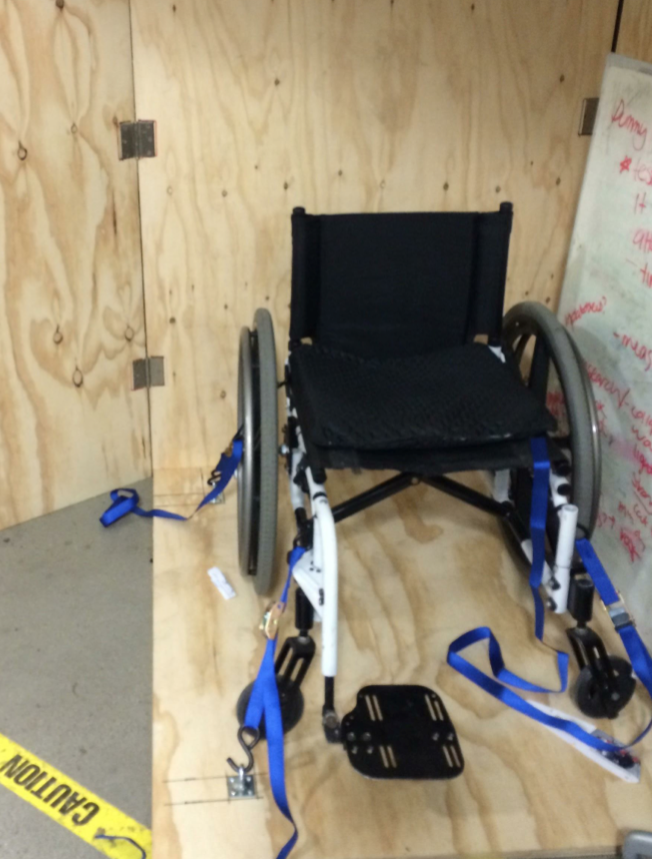
\includegraphics[width=7cm]{images/wheelchairprototype1.png}
   \caption{First prototype of wheelchair storage device.}
  \label{fig:wheelchairprototype1.png}
\end{figure}

Since many of the stories we encountered about wheelchairs being damaged involved airport personnel attempting to disasemble them or handling them poorly, we wanted the wheelchair owner to be present during the securing process, just like they are on a bus or train. This way, the wheelchair user could help the airport personnel speed up the process by providing information about their specific wheelchair and how it should be secured as well as ensure that the airport personnel is not accidentally mishandling their mobility device. At the end of the securing procedure, the container is to be closed up, giving the user feeling satisfaction in knowing that their wheelchair is secure and will arrive safely at their destination. 
 
Part of having the wheelchair user present while their wheelchair is secured is also enabling an easy transfer from their personal wheelchair onto the aisle chair. As shown in the rendering  Figure \ref{fig:storagetransfer.png}, right now this is accomplished by bringing the transferchair close to the passenger's chair that is already secured. This further explains our use of hinged walls and puts a hard constraint on our system- in order for the wheelchair user to be able to easily transfer once their wheelchair is secured, there must be a way to ``remove'' all walls during securing and ``reappear'' them for the wheelchair to be protected.

\begin{figure}[h]
  \centering
     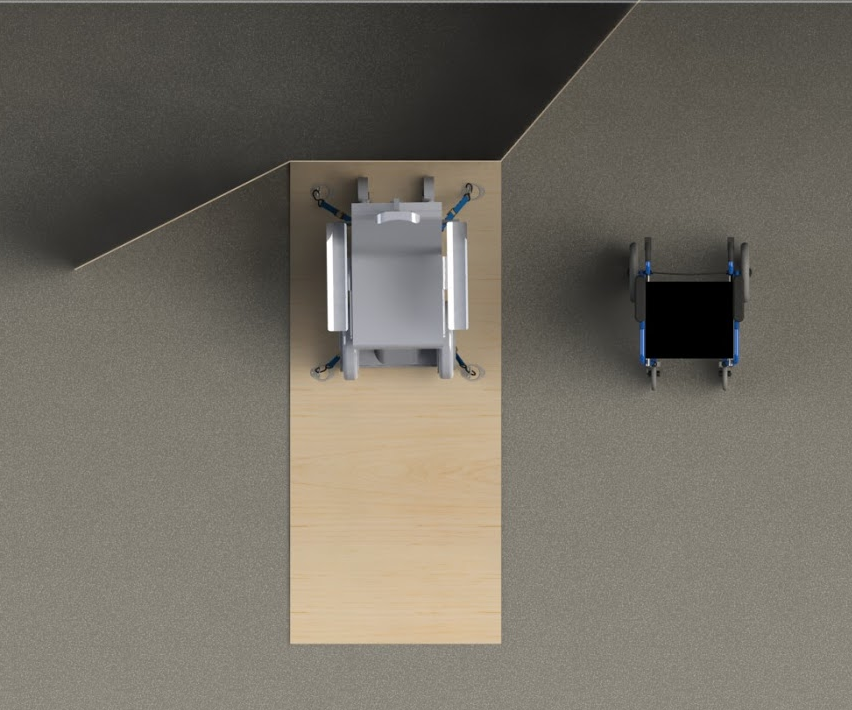
\includegraphics[width=7cm]{images/storagetransfer.png}
   \caption{Rendering of wheelchair and aisle chair side by side once wheelchair has been secured.}
  \label{fig:storagetransfer.png}
\end{figure}

While there are certain hard constraints that were not met with this protoype, we are keeping them in mind and will insitute them in future iterations. We know the container must protect the wheelchair but also fit through the door to the cargo hold as well as fit inside the cargo hold. It needs to be movable, as the wheelchair storage container must travel from the jetway down into the cargo hold. This product must help the luggage handler create a connection with the wheelchair user and gain empathy for the importance of the mobility device that is in their hands; the more important they know it is, the better they will treat it. Finally, the storage device must be lightweight as this is of utmost importance to Embraer.

\subsection{Wheelchair Storage Learnings \& Next Steps}

From our first prototype we were able to learn a myriad of things. Primarily, we realized that using a mechanism that wheelchair users are already familiar with is a huge plus; it provides them with a feeling of trust and security that their wheelchair will not be damaged throughout their flight. Thus, we suceeded at providing the user peace of mind with this device. However, we realized it is pretty difficult to line the chair up in the correctly in between the hook protruding out of the base and thus it would be best to have the hooks be flush against the top of the base so they didn't get in the way of the wheelchair manuevering.
We had several users go through the process of securing the wheelchair and found that having simple straps and hooks can be confusing and time consuming. Thus, it is best to have retractable hooks that come out of the base so that the tension is automatically set, making the job of the securer much easier. 

For a process that takes place prior to a flight, time efficiency is extremely important. Airport personnel are very crunched for time as they cannot afford to have any process delay the flight and push their schedules back. This means having very clear instructions for both the wheelchair user as to what's expectedof them, where to park and how the process will unfold, as well as for the person securing the wheelchair. For the wheelchair user, we are thinking of ways to transfer this imformation prior to their flight, knowing that most disabled passengers keenly do their research before flying. Having a video that shows the whole process would allow the wheelchair user to be prepared to tell the securer exactly what the right attachment points are and how to best secure the wheelchair down. On the other hand, it is important for the securer to know the correct order of the procedure which can be accomplished by numbers next to each hook as shown in Figure \ref{fig:instructionsstorage.png} and simple drawings depicting what's next. 

\begin{figure}[h]
  \centering
     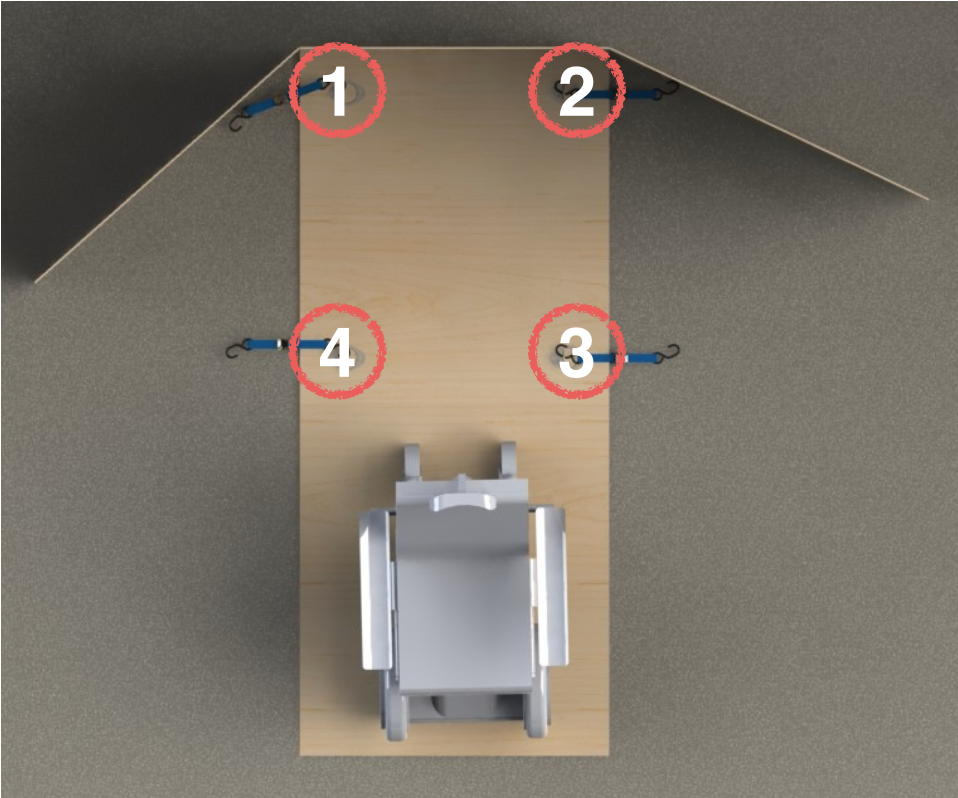
\includegraphics[width=7cm]{images/instructionsstorage.png}
   \caption{Tweet from Josie Verguese about her experience when her wheelchair did not make it to her destination.}
  \label{fig:instructionsstorage.png}
\end{figure}

Finally, our user testing confirmed our theory that we would need retractable walls. Not only were they necessary for the user to easily transfer onto the aisle chair but they also made the securing process much easier. The back wall, however, was still rigidly attached. This, we found, was not ideal as it made the two hooks in the back extremely hard to reach. With this information in mind, we have been brainstorming different design ideas that would enable for the walls to be completely out of the way during boarding and securing yet would be present during flight to protect the wheelchair from being damaged. We have thought about accordion or telescoping walls as well as having inflatable walls. We really liked the idea of inflatable walls as it provided the wheelchair with protection from damage yet could be blown up to accomodate different types of wheelchair sizes and would be extremely light weight. A preliminary mock up of a possible vision can be seen in Figure \ref{fig:inflatablesrendering.png} With this in mind, we began a feasibility study to understand how possible the use of inflatables would be in the application. 


\begin{figure}[h]
  \centering
     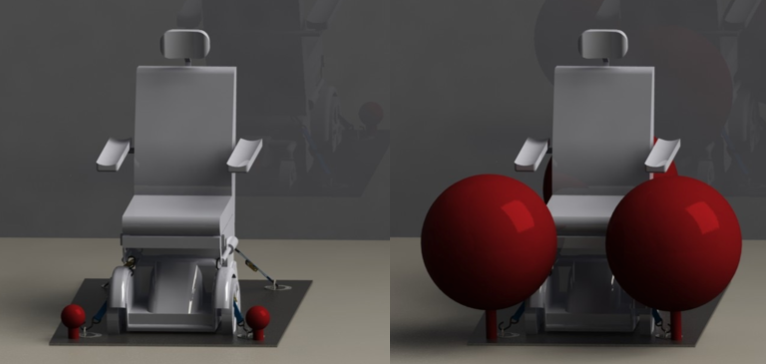
\includegraphics[width=7cm]{images/inflatablesrendering.png}
   \caption{Rendering of a preliminary idea of what an inflatable ``wall'' could be.}
  \label{fig:inflatablesrendering.png}
\end{figure}

%take it from here robbie!











\subsubsection{Inflatable Materials}

\textbf{Inflatable Materials}
In order to test the feasibility of an inflatable device in the cargo hold there were a few problems that needed to be addressed. 

\subsection{Wheelchair Tracking}

\subsubsection{Pressure}
The cargo hold of many planes is not pressurized in order to save on costs. One of our goals was to determine if an inflatable device to protect the wheelchair would pose a problem in low pressure situations. Initially we were unsure as to what the pressure in the cargo hold would be, and as such decided to design for the worst case when the pressure is the same inside the cargo hold as outside. \\

It was important to design for this case as regardless of the pressure in the cargo hold, in any emergency situations where the cabin lost power, we would not problems to arise in the cargo hold potentially making the situation worse.

\subsubsection{Temperature}
A second potential problem with an inflatable device in the cargo hold is that the luggage does not require the same heating and insulation as passengers. While it may not get as cold as the air outside (approximately -40 C) in normal situations, as in the pressure situation the device must be designed reliably for an emergency. \\

\subsubsection{Testing}
While it may be possible to test the effects of pressure on an inflatable device without taking it into a plane by increasing the pressure inside the inflatable device since the pressure differential is the most important aspect to test. However, its much more difficult to test this pressure differential at a realistic temperature on the ground. Instead we decided it would be best to get an inflatable structure up to approximately the height of a plane and determine what failure modes if any would be present. \\

In order to do this we attached an arm flotation device fully filled to a weather balloon. This balloon was released in order to take the device into the upper atmosphere where it would experience similar conditions to those of an airplane. While it ignores some effects from the natural plane insulation, its a more extreme environment in all cases so its a good measure of feasibility. \\

\subsubsection{Results}
Unfortunately the barometer which was being used as an altimeter for this experiment failed, and as such we were unable to get reliable altitude data on the flight. However by looking at the videos returned from the launch, and given the groups prior experience with weather balloons a reasonably reliable estimate of 50,000 - 60,000 ft can be estimated for when the flotation device popped which is significantly higher than an embraer jet flies (37,000 ft maximum). We were able to see small water droplets on the larger weather balloon which froze at altitude forming ice crystals.


\subsection{Wheelchair Tracking Concept}

%\section{Brainstorming}
%The problem statement provided by Embraer gave a great deal of direction to our brainstorming sessions including the two parts of the team (Stanford and USP).  The design space concerned two potential users: limited mobility or disabled passengers and the flight crew.  The need-finding and benchmarking phases began with looking at the perspective of the disabled passengers and what is out there for them in the current system.  The flight crew perspective brought restrictions on the design space by limiting the system to being controlled by the flight crew and fitting to their needs and motivations as well.
%
%\begin{figure}[h]
%  \centering
%     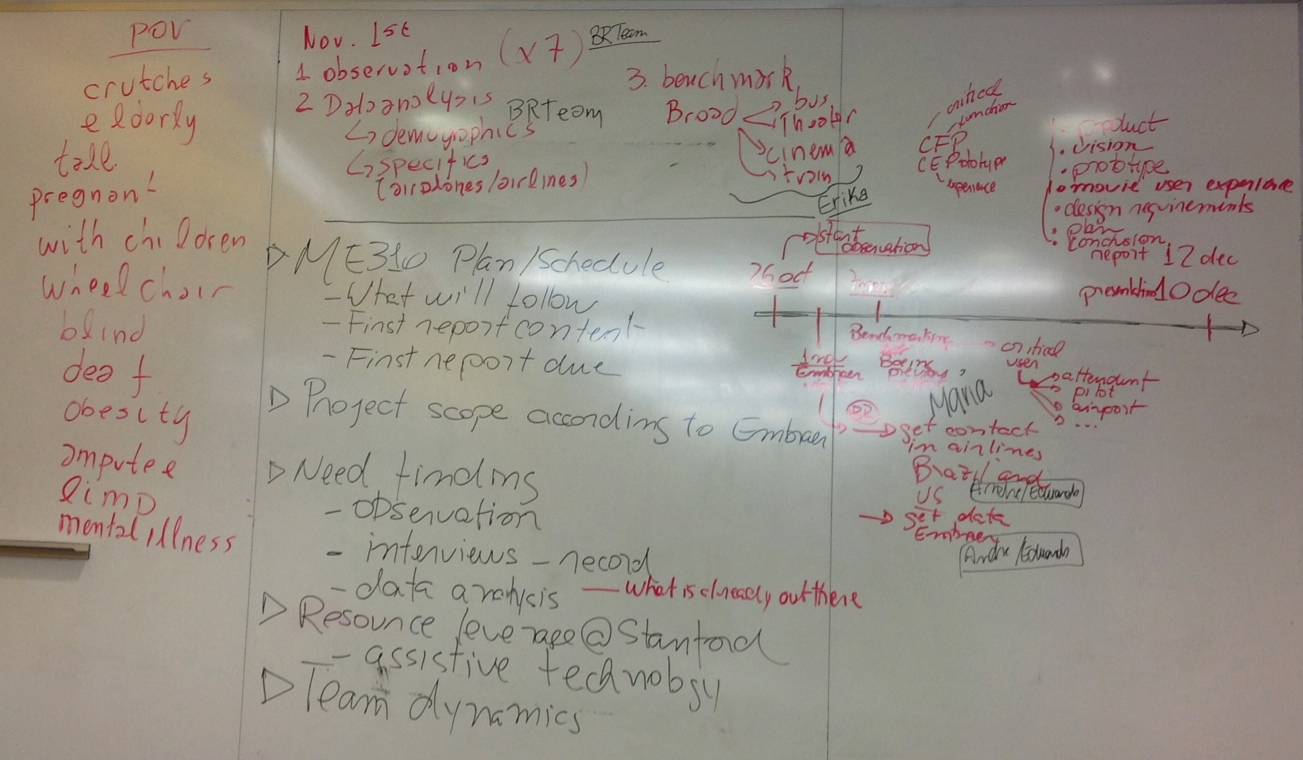
\includegraphics[width=7cm]{images/image017}
%   \caption{Initial brainstorming with the whole team (USP and Stanford).}
%  \label{fig:17}
%\end{figure}
%
%The first brainstorming session was held with our global team during global kick-off week.  Figure 3 1 shows the product of the first session and the task assignments for each team.  The session focused on the first deliverables that were due, who the potential limited mobility passengers could be, what places could be researched for benchmarking, and the data that could be useful to justify persona and potential users.
%
%The second main brainstorming session centered on determining the entire system of the flight experience and what sections could be improved the most. Figure 3 2 shows the brainstorming session in progress.  This session utilized sticky notes to determine mandatory and optional activities that needed to be addressed within the design space. This was the final brainstorming session that was held jointly with both team parts.  The USP and Stanford team members all worked together to develop the chart composed of sticky notes in Figure 3 3, which addresses every aspect of the travel experience from leaving home and arriving at the airport, going through security and getting to the gate, getting food and drinks while in the airport, using the restroom, boarding the plane and the in-flight experience, and finally baggage claim to final destination.
%
%\begin{figure}[h]
%  \centering
%     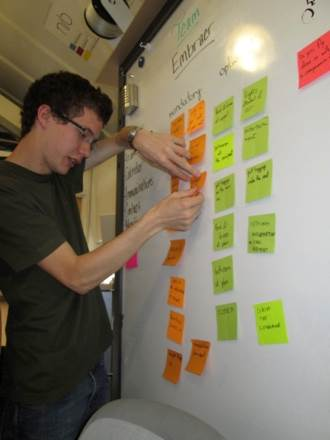
\includegraphics[width=7cm]{images/image018}
%   \caption{Brainstorming session used to map out entire flying experience.}
%  \label{fig:18}
%\end{figure}
%
%The remaining brainstorming sessions took place in more conversational format with note taking.  The notes were centered on the interviews and individual research each team member had conducted.
%
%\section{Communication}
%\begin{figure}[h]
%  \centering
%     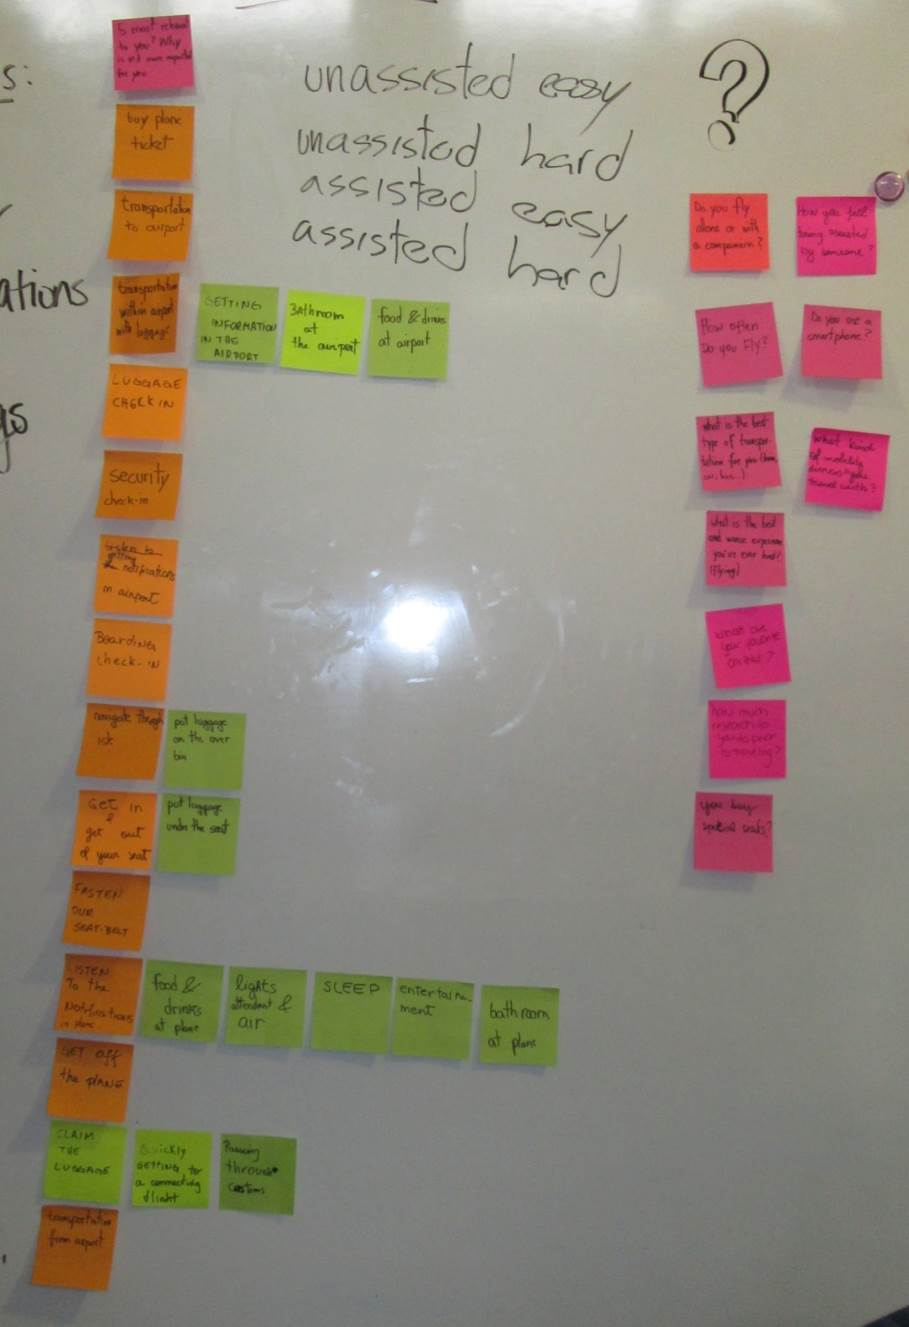
\includegraphics[width=7cm]{images/image019}
%   \caption{Completed brainstorming displaying every step of the flying experience.}
%  \label{fig:19}
%\end{figure}
%
%The communication for our team is done primarily through two main channels.  First, we have weekly Skype meetings to discuss what was done within the last week and what needs to be done for the next week as well as to present future deliverables.  Our second mode of communication is Podio, an online work platform for collaboration and project management where we can assign tasks, discuss projects, upload files, share findings, and communicate with status updates. These software tools allow us to keep all the major findings in one place and allow us to share what we are doing real-time.  Common applications such as Dropbox, Google Docs, and Google Forms are also being used as need be to share ideas, findings and important documents. 
%
%\section{User Benchmarking and Need-Finding}
%The first deliverable of the fall quarter concerning our corporate project was the benchmarking and need-finding deliverable.  Current systems and technology were to be researched to see what is available to complete the benchmarking task.  User interviews and user personas were to be conducted and developed, respectively, to inform our team and audience on what needs our solution needs to be addressing. 
%
%\section{Need-Finding}
%The solution to a problem needs to address the gaps that exist within the current systems. In order to find these gaps, our team had to extensive need finding by conducting user interviews with different potential users as well as experts in the field.  Each interview gave us some more detail into who our user would be and how to go about developing our personas.
%
%\subsection{Expert Interviews}
%To begin the need-finding process, we wanted to investigate what research projects had been pursued within the aerospace industry. Two experts, one from Boeing and the other from Oregon State University shared their work experience and its motivation with us. 
%
%\subsubsection{Dianne McMullin, Human Factors Engineer at Boeing}
%\begin{figure}[h]
%  \centering
%     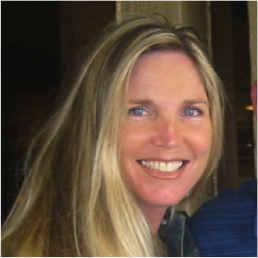
\includegraphics[width=7cm]{images/image020}
%  \label{fig:20}
%\end{figure}
%
%Dianne McMullin is a technical fellow in Human Factors Engineer at Boeing and worked on the 787 Assistive Technology Design.  She has been working on this problem for over 15 years.  Since she is currently working on a project with Embraer to better the flying experience for the aging passenger, she had a lot of fresh knowledge that proved to be very relevant to our work. She shared with us some of the major restrictions we need to be conscious of such when designing something for the airline industry. These include:	
%\begin{list}{-}{}
%  \item Maintain the number of seats. Airlines, and consequently airplane manufacturers, want the maximum number of seats possible to maximize profit.
%  \item While in the air, space is more expensive than most expensive real estate in Tokyo, minimizing size is paramount.
%  \item Weight is a critical factor, a solution cannot significantly add weight to the aircraft.
%\end{list}
%
%She was also able to share with us some touching points that she had encountered in her research and work.  These two aspects made the team think about our users in a new light and helped us empathize with the situation and feel the pain.  
%
%\begin{list}{-}{}
%  \item The utter sense of despair and helplessness when cane/crutches is taken away.
%  \item Not traveling can mean not seeing kids or grandkids, missing weddings and vacations. It literally means giving up a piece of their life. Making this a better experience can, in essence, give back a little piece of that.
%\end{list}
%
%\subsection{Kate Hunter-Zaworksi, Director of National Center for Accessible Transportation}
%\begin{figure}[h]
%  \centering
%     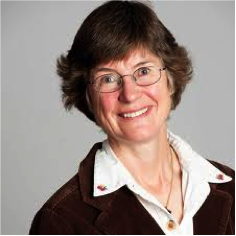
\includegraphics[width=7cm]{images/image021}
%  \label{fig:21}
%\end{figure}
%Kate Hunter-Zaworski is the Director of the National Center for Accessible Transportation and also worked with Boeing on the 787 Assistive Technology Design.  She was able to give us some more places to contact, interesting facts that could be used to implement a design solution, and areas to start brainstorming.  Below is some of the food for thought she left us with:
%
%\begin{list}{-}{}
%  \item When considering the possibility of tying down wheelchairs within the cabin, the wheelchair’s impact capabilities are of prime concern. However, some wheelchairs are able to stand up to 20Gs while airplane seats can only support 16Gs.
%  \item Folding canes and other mobility aids that can be stored within the cabin and remain accessible are interesting solutions to consider. 
%  \item Why can’t you maneuver a wheelchair with only one hand?
%\end{list}
%
%\subsection{User Interviews}
%User interviews were used to really get a sense for what the user experience was, allowing us to no longer rely on our own assumptions. Given that the problem statement does not state a type of disability to focus on, we strived to encompass as many different types of disabilities as possible, looking for overlaps within the experiences. The interviews not only gave us insight into where the pain point lie but also humanized the problem even more for us. Being able to talk to these users who both have to deal with these issues on a daily basis but are also invested in helping others navigate the traveling process was extremely rewarding. Their passion for the subject refueled our own. 
%
%\subsection*{Wheelchair Users}
%The motivation behind these interviews was to find areas where corrective actions can be implemented during the travel experience for a person in a wheelchair.
%
%\subsubsection{Teri Adams, Assistant Director of Stanford Office of Accessible Education}
%\begin{figure}[h]
%  \centering
%     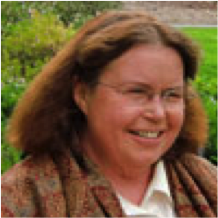
\includegraphics[width=7cm]{images/image022}
%  \label{fig:22}
%\end{figure}
%
%Teri Adams is the Assistant Director of the Stanford Office of Accessible Education.  She is an avid traveler and utilizes a power wheelchair every day and a manual wheelchair on trips. She used to travel with her power wheelchair but stopped after having several instances where her chair came back from the cargo hold broken. The following are the main areas she highlighted within her interview:
%
%\begin{figure}[h]
%  \centering
%     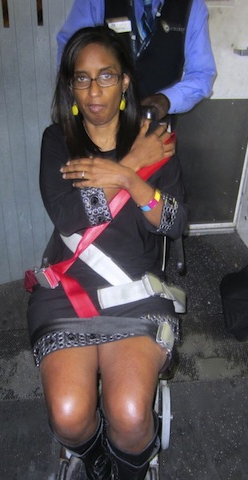
\includegraphics[width=7cm]{images/image023}
%   \caption{Nicole Lemelle has Multiple Sclerosis and needs ad aisle chair to board the plane. Source: http://www.mynewnormals.com/aisle-chair/}
%  \label{fig:23}
%\end{figure}
%
%\begin{list}{-}{}
%  \item Highlighted the persistent problem of wheelchairs being broken, both in her experience as well as her friends'.
%  \item Described the aisle chair used to move wheelchair users from their wheelchair into the airplane seat if they cannot do it themselves. It is an incredibly degrading and embarrassing process, as shown in Figure 3 4 because the chair is not designed to fit an average sized person. Usually the process takes place before boarding begins.
%  \item Addressed the important issue of customer service's impact. The most dramatic horror stories she had came from a lack of training or knowledge from the flight crew.
%  \item Enlightened us on the reality of seat preferences. We assumed that people with disabilities would always choose to sit by the aisle due to the ease of access but actually found that many prefer to sit in the window seat so that they do not have to get up and down every time someone from their row needs to walk around the cabin. This is something that was completely new to us.
%  \item Emphasized the difficulty of reaching the controls while in flight and the need for a more accessible and intuitive placement for them. 
%\end{list}
%
%\subsubsection{Scott Rains, Travel and Cruise Specialist for Disabled Persons}
%\begin{figure}[h]
%  \centering
%     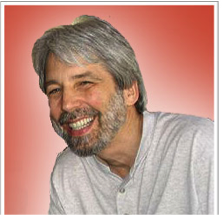
\includegraphics[width=7cm]{images/image024}
%  \label{fig:24}
%\end{figure}
%
%Scott Rains is a paraplegic who is very passionate about the subject of disables traveling. He is a travel and cruise specialist and an avid travel blogger, providing a community of people with disabilities with tips on how to best navigate using the current solutions out there.  He travels multiple times a year for work and pleasure.  Scott was kind enough to connect us with multiple contacts that we were able to reach out to due to his wealth of knowledge on the subject matter.  The following were the main points that he stressed needed to be included in our design solution: 
%
%\begin{list}{-}{}
%  \item Surprisingly, hinged armrests are not the standard. There are many aircraft where they are not present, making the transfer of a disabled passenger infinitely more difficult. He recounted a friend’s experience of getting bumped into the armrest and needing to spend 2 weeks in the hospital as a result of the sore caused by the bump. 
%  \item Even if hinged armrests are present, the hinges are often hard to find and the flight attendants are not familiar with how to operate them. It follows with other accessibility features such as additional seat belt extensions for lumbar support.
%  \item All disabilities are different and thus they need different things. Wheelchair users often have customized cushions or seat pads that allow for more comfort. This type of solution should also be implemented in long duration flights. If people bring their own neck pillow, why not their own butt cushion?
%  \item Reemphasized disabled passengers’ wishes to sit in the window seat also for the support the wall provides as well as not wanting to be disturbed when others need to walk around the cabin. Lack of accessible controls was also mentioned. 
%\end{list}
%
%\subsubsection{Jose Luis Naranjo, T6 Paraplegic}
%\begin{figure}[h]
%  \centering
%     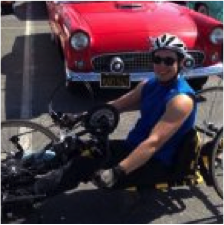
\includegraphics[width=7cm]{images/image025}
%  \label{fig:25}
%\end{figure}
%
%Jose Luis Naranjo is a 28-year-old T6 paraplegic.  He studied engineering at MIT and now works in the bay area as a mechanical/aerospace engineer.  He gave us his view of the situation and applied his engineering knowledge to help us brainstorm other solutions.  His focus points were the following:
%
%\begin{list}{-}{}
%  \item Wheelchair storage in the cargo hold is extremely poor, they literally just throw the wheelchairs in there which allows them to shift around during flight. Very often chairs are broken. 
%  \item Flight crew also does not know how to operate the wheelchairs and have tried to fold a non-foldable wheelchair before, resulting in damaged wheelchairs.
%  \item He uses the aisle chair very often and has noticed that because the center of gravity is very high on the aisle chair, it’s very easy to flip over and there is little sense of control.
%  \item Sometimes only one side of the airplane has folding armrests. 
%  \item Boarding processes are extremely rushed, the flight crew’s main priority is to get the plane out on time which has a huge impact on how much time they spend with the disabled passengers that need assistance. 
%  \item Keeping track of belongings is extremely difficult, you must rely on a flight attendant to carry your luggage and then remove all loose items from the wheelchair prior to storing it. This lack of independence and control over one’s belongings is nerve-wracking.
%  \item He is a frequently traveler and thus is aware of the preparations he must ensure before each flight, especially assuring that he does not have to use the restroom at any point. 
%  \item A solution must allow for people to do as much as they can themselves, returning that lost sense of independence and control. “What little mobility I have left, I want to use.”
%  \item A solution must ensure that disabled passengers are not being segregated from the rest of the population. They already know they’re different, they don’t need to be reminded. Inclusivity is key. 
%\end{list}
%
%\subsubsection{Cid Torquato, Municipal Department of People with Disabilities and Reduced Mobility}
%\begin{figure}[h]
%  \centering
%     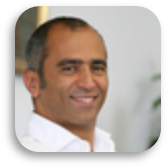
\includegraphics[width=7cm]{images/image026}
%  \label{fig:26}
%\end{figure}
%
%Cid Torquato is the Coordinator at the Municipal Department of People with Disabilities and Reduced Mobility in Sao Paulo, Brazil. He is paraplegic, and constantly travels to several countries due to his responsibilities in the department. The main points of the interview are as follows:
%
%\begin{list}{-}{}
%  \item There are many difficulties applying the law, people simply do not want to follow it.
%  \item There is a lack of proper training (and even good will) for many people involved in the flight experience.
%  \item There are some alternatives to the use of bathrooms for people with reduced mobility, including drastic ones like using a catheter to collect urine, diapers or even plugs. Due to the discomfort of using these solutions, people still prefer to use the airplane bathroom.
%  \item Usually, security will just use the hand metal detector and will not ask for the disabled to get up off the wheelchair. However, the interviewee had an awful experience during one of his travels where they forced him to do so, even though he cannot move. He had to make his companion make a space between his back and the chair to show to security there was in fact, nothing to hide.
%  \item Some airlines use contractors to handle people with disabilities, where trained people help with transportation and other needs of the passenger.
%  \item There is a lack of precise information about what can or cannot be done while boarding a reduced mobility passenger. Sometimes the airline does not allow the passenger to take his/her own wheelchair through the jet way to they airplane, stating that only the airport wheelchair is allowed even though the common procedure is to pull up at the front door of the airplane and change into the aisle chair. 
%\end{list}
%
%\subsubsection{Nanci Linke-Ellis, Board of Trustees for HLAA}
%
%\begin{figure}[h]
%  \centering
%     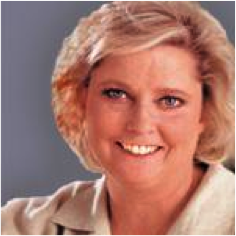
\includegraphics[width=7cm]{images/image027}
%  \label{fig:27}
%\end{figure}
%
%Nanci Linke-Ellis is on the Board of Trustee for Hearing Loss Association of America and is a deaf traveler. She was able to give us more information about where corrective actions could be applied in the travel experience specifically concerning the deaf passenger. These are some of the problems she brought to our attention more than before:
%
%\begin{list}{-}{}
%  \item The customer service element is absolutely huge and causes a great deal of problems. Once, she approached the gate agent to inform her that she was deaf and would need to be notified of any announcements. The gate agent then asked her if she needed a wheelchair. Flight attendants do not know how to react or are uneducated about dealing with persons with disabilities. 
%  \item As a disabled traveler, it is important to make the flight crew aware of the problem but also present a possible solution. 
%  \item Planes, airports, terminals, etc. need more signage and to be more visual with instructions. This not only affects the deaf but also all passengers struggling to hear information over the loud background noise found in airports. Using a smartphone app could be an interesting solution
%  \item Increasing independence is key. 
%\end{list}
%
%\subsection*{Blind User}
%\subsubsection{Cheryl Echevarria, President of NFB Travel and Tourism Division}
%\begin{figure}[h]
%  \centering
%     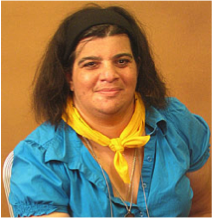
\includegraphics[width=7cm]{images/image028}
%  \label{fig:28}
%\end{figure}
%
%Cheryl Echevarria is the President of NFB Travel and Tourism Division and owns her own travel agency that specializes in assisting blind travelers.  She shared with us the independence that blind persons have while travelling due to advancements in education for the blind and support for the blind as well as assistive technologies that are available.  She highlighted some of the main points that were already suggested by our previous interviews adding the following:
%
%\begin{list}{-}{}
%  \item Customer service is a major factor that can make or break an experience. The disabled person must be aware of the rules and be willing to teach uneducated flight crew about what is allowed during flight (such as leaving your cane under your seat). Blind people would most likely not be a target user given the range of technologies already available.
%\end{list}
%
%\subsection{Flight Crew}
%
%\begin{figure}[h]
%  \centering
%     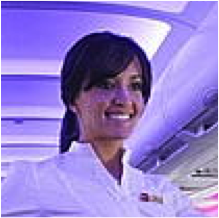
\includegraphics[width=7cm]{images/image029}
%   \caption{Nikole Rubyn Virgin America Founding Flight Attendant}
%  \label{fig:29}
%\end{figure}
%
%\begin{figure}[h]
%  \centering
%     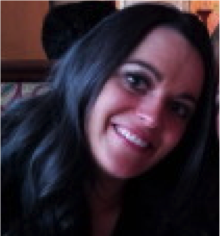
\includegraphics[width=7cm]{images/image030}
%   \caption{Dena Silva-Heath Alaska Airlines Flight Attendant}
%  \label{fig:30}
%\end{figure}
%
%\begin{figure}[h]
%  \centering
%     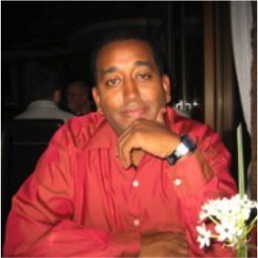
\includegraphics[width=7cm]{images/image031}
%   \caption{Yonatan Godefa Virgin America Gate Agent}
%  \label{fig:31}
%\end{figure}
%
%Interviewing potential users made us realize there were also other major stakeholders that had to be considered when designing a solution: the cabin crew. Not only does the cabin crew have to interact with disabled passengers on an every day basis but their actions are often fueled by motivations that can contradict providing the best assistance possible to the disabled passengers. We spoke with two flight attendants and a gate agent to get a better sense of what their pain points were, what they perceived the pain points to be for the disabled passenger and their motivations when executing tasks on the job. These findings can be broken down into two different areas of concern, the airports and the airplane. 
%
%\subsubsection{Airport}
%\begin{list}{-}{}
%  \item Not all the airports are ready to receive disabled passengers; some do not have the appropriate equipment or personnel.
%  \item Some airports do not have enough equipment for disabled. Once, one of the flight attendants waited 40 minutes for the lift, “airport elevator on the runway”, to disembark the disabled.
%  \item The aisle chair is too small for most passengers.
%\end{list}
%
%\subsubsection{Airplane}
%\begin{list}{-}{}
%  \item Not all the armrest are retractable, in some aircraft just the ones on the first and the second rows are.
%  \item The lavatory is too small for the aisle chair, so often the disabled have to use it with the door open.
%  \item For blind people they can provide the safety procedures in Braille. Little known fact, however, is that not many blind people actually know Braille.
%  \item For deaf people there isn’t any special equipment, the crew members have to speak really close so the disabled can read their lips. 
%  \item People with no chest mobility can use a special belt, but sometimes the family doesn’t want it or the flight crew isn’t aware of its existence.
%  \item Paralympics athletes can usually get to their seat on their own and thus they can allow more disabled passengers on the plane when they’re flying. Usually the number allowed is one third of the number of crewmembers.
%\end{list}
%
%\subsubsection{Miscellaneous}
%\begin{list}{-}{}
%  \item The disabled feels humiliated for being carried thought the aisle.
%  \item A recently disabled person is usually more dependent and more uncomfortable with the situation.
%  \item Many people do not prepare sufficiently for the flight. They either do not have credit cards to purchase food onboard or don’t realize they should go to the bathroom beforehand. The gate agents can play a role in aiding passengers prepare. 
%  \item The flight crew has another 140 passengers they must cater to throughout the flight, making it impossible for them to dedicate a significant amount of time to assisting disabled passengers.
%\end{list}
%
%\subsection{Observations}
%In order to get a complete picture of what the traveling experience entails in general as well as how it differs for disabled passengers, our team decided to use their travels as an opportunity to delve deeper into the topic. Six different people from USP made many of the following observations on October 2013. Both the teaching team and the students travelled from Palo Alto to São Paulo (GRU) via San Francisco (SFO) or San Jose (SJO) with connections in Dallas (DFW). Most of them were on different flights and got to experience different situations. Included are also observations conducted by the Stanford team during their flight home for Thanksgiving.
%
%\subsubsection{Outside the Airport}
%\begin{list}{-}{}
%  \item It is difficult to find a cab in smaller cities (an accessible taxi would be even more difficult).
%  \item Walking within the city of Palo Alto was not a good experience, especially because sidewalks suddenly disappeared without any indication whatsoever. Urban planners really must take people with disabilities into account when designing urban layouts.
%  \item Ticket vending machines at Caltrain/BART are not suited for people with disabilities, it would be extremely hard for someone in a wheelchair to reach and purchase a ticket.
%  \item Lack of signage makes it very difficult to travel by train, especially if one has any hearing loss (or doesn’t speak English fluently).
%  \item The train and bus used to get to the San Jose airport do not offer adequate space for storing luggage near the seats reserved for people with disabilities.
%  \item Getting in and out of the train is difficult because of the stairs and also because of the short time to embark.
%  \item There are no people assisting passengers to embark the train/bus.
%  \item There are not sufficient handles to hold on to on the train. This is a huge issue if one does not have perfect balance. 
%\end{list}
%
%\subsubsection{Inside the Airport}
%\begin{list}{-}{}
%  \item There are some boarding assisting areas inside the airport and dedicated waiting lines for people with reduced mobility, as seen in Figure 3 5.
%
%\begin{figure}[h]
%  \centering
%     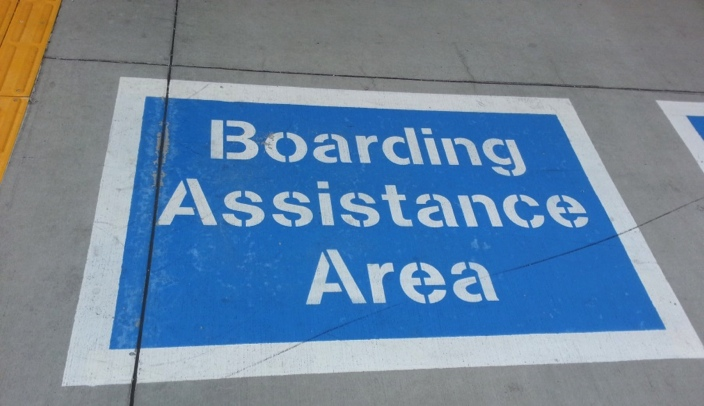
\includegraphics[width=7cm]{images/image032}
%   \caption{From L to R: Boarding assistance area and dedicated waiting line}
%  \label{fig:32}
%\end{figure}
%\begin{figure}[h]
%  \centering
%     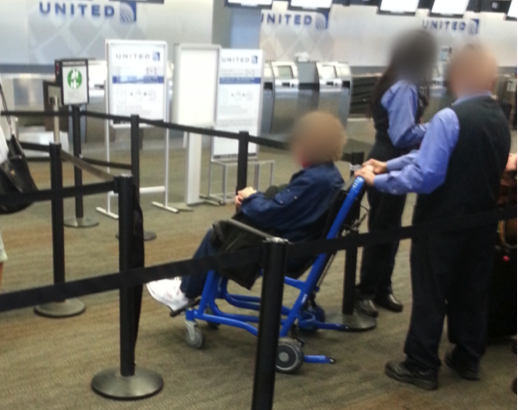
\includegraphics[width=7cm]{images/image033}
%  \label{fig:33}
%\end{figure}
%
%  \item Finding the airline counter is not trivial, especially if one has a poor vision or is not familiar with the airport layout. There is not enough information displayed to make it an easy task.
%  \item Check-in counters are not adapted for people with special needs. 
%  \item Conventional check-in counter is too high for a person in a wheelchair. The electronic kiosk is not user-friendly and may only be operated by a person standing and that can see. Furthermore weight scale is above the floor level, requiring somebody to lift the luggage. Assistance is provided when requested but a lot can be done to improve the process.
%  \item Due to recent lawsuits, the Transportation Department is now requiring that all new kiosks be made accessible and that all existing kiosks must be converted within a 10 year time period.  This is a huge step forward for allowing people with disabilities to have a better flying experience.
%  \item The large mount of paper and documents required for taking a plane makes it easier to misplace something important in airport. Remember, people are normally stressed in airports.
%  \item There are few places to wait before the security check-in and the existing ones do not have reserved seats for disabled.
%
%\begin{figure}[h]
%  \centering
%     \includegraphics[width=7cm]{images/image034}
%   \caption{From L to R: Wheelchair with small wheels, with big wheels and for aisle}
%  \label{fig:34}
%\end{figure}
%\begin{figure}[h]
%  \centering
%     \includegraphics[width=7cm]{images/image035}
%  \label{fig:35}
%\end{figure}
%\begin{figure}[h]
%  \centering
%     \includegraphics[width=7cm]{images/image036}
%  \label{fig:36}
%\end{figure}
%
%  \item There are at least three types of wheelchairs like those in Figure 3 6 in an airport: those with small wheels which require someone else to push it, thus limiting the passenger’s independence, those with larger wheels that provide some level of independency since the passenger can conceivably wheel themselves around and aisle wheelchairs which are used for transporting passengers from a wheelchair in the jet way to their seats on the airplane.
%  \item One is normally required to walk long distances to reach one’s gate. However, the airports we visited mitigated that problem by offering solutions like an electric cart that can carry up to 12 people (including the driver) and small buses for transportation outside the building, both shown in Figure 3 7.
%
%\begin{figure}[h]
%  \centering
%     \includegraphics[width=7cm]{images/image037}
%   \caption{From L to R: Cart for inside transportation and bus for outside transportation}
%  \label{fig:37}
%\end{figure}
%\begin{figure}[h]
%  \centering
%     \includegraphics[width=7cm]{images/image038}
%  \label{fig:38}
%\end{figure}
%
%
%  \item Finding the boarding gate can be a problem especially with last minute time changes, the increasing distance between gates and the difficulty of listening to the airport’s sound system.
%  \item Removing all belongings when passing through security may be very difficult for some people. Although it is true that there is a special procedure for people with disabilities, the elderly did not have a special treatment.  The conveyor belt is too high, making it hard to place heavy belongings on the table. Plus, there is a lot of added social pressure to move extremely fast.
%  \item It is very difficult to understand the airport’s sound system over the loud background noise, even if one has a good hearing.
%  \item Some wheelchair users have to change wheelchairs more than once in airport during check-in and boarding.
%  \item Finding one’s luggage and picking it up on baggage claim area is not as easy as one might imagine. The conveyor belt moves fast and the weight of the luggage is elevated, making it hard for someone with less than perfect mobility to easily achieve the task. Most of the time, there are no employees helping.
%
%\begin{figure}[h]
%  \centering
%     \includegraphics[width=7cm]{images/image039}
%   \caption{Obese person being transferred from wheelchair to taxi.}
%  \label{fig:39}
%\end{figure}
%
%  \item Although there a lot of taxis in airports, finding one that is accessible to people with reduced mobility is not as easy as one might expect. As a result, these people have to be assisted (and touched) by other people as seen in Figure 3 8.
%\end{list}
%
%\subsection{Airplane Observations}
%\begin{enumerate}
%  \item There should be an indicator to inform passengers if overhead luggage bin is full.
%  \item Seat numbers should be marked more clearly because the numbers are too small.
%  \item The food tray is very slippery causing contents to go rolling all over the place during flight. A better design would include a non-slippery surface.
%  \item Attendant, light buttons and air control should be accessible and more intuitive to everyone. For a lot of people, it is very hard to reach all the way to the ceiling to press these buttons. In some aircraft, there is a button closer to the seat but unfortunately it is very difficult to see it. In other aircraft, the buttons are on the arm rest and get pressed accidentally all the time. 
%  \item Seatbelts should be retractable to avoid tangling.
%  \item Economy class seats need to be more ergonomic to provide more comfort for users, particularly for spine and lumbar support.
%  \item Seats should have footrests to improve comfort for everyone and especially for shorter people. 
%  \item The first row of seats should be more accessible to people with disabilities; the armrest should not be fixed since wheelchair users prefer to use these seats and aisle chair transfer is extremely difficult with an armrest in the way. 
%  \item It is very difficult to understand pilot speaking in the airplane.
%  \item The WC was not adapted for people with reduced mobility, it was small and cramped. 
%  \item The height of the luggage bin makes it very difficult for everyone to store and retrieve a bag, especially for shorter people.
%  \item  A suitable place to wait to go to the lavatory does not currently exist,  you are often blocking the aisle and hindering others from getting by you. 
%  \item It is not possible to walk through the aisle when food is being served because of the dimensions of the cart/aisle.
%  \item Attendants don’t provide enough time to eat. 
%  \item Seats are not designed for children.
%  \item There are no proper areas do dispose trash while seated (unless a flight attendant is walking by with a trash bag).
%  \item In the lavatory it is not clear where each type of trash should be disposed where.
%  \item The seat is too high for people with a short stature.
%  \item The seat is too tight for obese people.
%  \item The conventional seat belt is too tight for obese people. Flight attendants need to offer seat belt extensions but a lot of them aren’t even aware they exist.
%\end{enumerate}
%
%In order to represent the key observations in a more visual manner, the diagram represented in Figure 3 9 was created. A magnified version can be found in the Appendix – Diagram A2.
%
%\begin{figure}[h]
%  \centering
%     \includegraphics[width=7cm]{images/image040}
%   \caption{Key observations diagram}
%  \label{fig:40}
%\end{figure}
%
%\section*{Persona Development}
%Our persona development was driven by our want to always keep the end user in mind. We recognize that this is a very human centered problem and want to ensure that we keep the human centered approach every step of the way. Through our interviews, observations and need-finding processes, we discovered our solution would actually have two critical users with very different problems and motivations. These users are Patty White, the grandma, and Juliette Fields, the flight attendant.
%
%\subsection{Patty White, The Elderly Passenger}
%
%\begin{figure}[h]
%  \centering
%     \includegraphics[width=7cm]{images/image041}
%   \caption{Patty White, one of our design personas}
%  \label{fig:41}
%\end{figure}
%
%We based Patty White, shown in Figure 3 5, on a compilation of characteristics from both our interviewees as well as characters in their stories. She is an older adult in her early 60s that has limited upper body strength and mobility. She is from Cleveland, Georgia and is a retired teacher. Her southern charm as well as her past experiences as an instructor make her a very well informed and easy going traveler, always eager to explain different rules and regulations because she is keen on helping the flight crew learn about people with disabilities. Patty is widowed and usually travels alone across the country to visit her grandchildren. For Patty, giving up on flying means giving up on family. She loves to cook and will often bring her family bags of baked and preserved goods as well as lots of toys for the kids, which means she usually travels with a lot of luggage.  Since Patty has just recently been dealing with her limited mobility, she is still learning to deal with being dependent on others. When flying, she is extremely uncomfortable because of the airplane seat’s lack of support and she needs to use the back of chairs to balance if she needs to move around the cabin.
%
%\subsection{Juliette Fields, Flight Attendant}
%
%The inspiration for our flight attendant arose from our many observations, past experiences and interviews. We know that the cabin crew plays an important part in the travel experience for disabled passengers and a great deal of horror stories comes from customer service issues. Thus, portraying this critical user and keeping their needs and motivations in mind is paramount as we design a solution. Juliette is in her late 20s, she doesn’t have a family and enjoys traveling around the world. She is fairly new to the airline industry and always follows protocol, she never goes above what is already listed. She does not have much experience with disabled passengers and is completely uneducated about their needs and abilities. 
%
%\section{Benchmarking}
%\section*{Analogous Solutions}
%Part of the benchmarking phase of this project dealt with looking into other transportation and recreational areas where solutions have been implemented to accommodate those with limited mobility.  Cinemas, public buses, mobility buses, personal vehicles, tram and train platforms, and grocery stores were all areas that were examined as analogous situations to the problem we were presented with.
%
%\subsection{Wheelchair and Passenger Transport}
%
%\begin{figure}[h]
%  \centering
%     \includegraphics[width=7cm]{images/image042}
%   \caption{Bus ramp used to assist entrance and exit onto bus. Source: http://www.romeinformation.it/en/guided-tours/rome-tours-for-disabled/}
%  \label{fig:42}
%\end{figure}
%
%Public buses were researched first when looking at wheelchair and passenger transport given that public bus systems service more cities than other modes of public transportation.  Figure 3 6 shows a ramp that is either pulled out or automatically released from under the doors of the buses.  This creates a safer and more convenient entrance onto the bus for passengers in wheelchairs or passengers that have a difficult time making the large step onto the bus. 
%
%\begin{figure}[h]
%  \centering
%     \includegraphics[width=7cm]{images/image039}
%   \caption{Lift used to assist in loading process.}% Source: http://www.beckettcorp.co.uk/index_files/vehiclesforhireandsale.htm}
%  \label{fig:39}
%\end{figure}
%
%Mobility buses or vans and personal vehicles were also examined as the accessibility features could be similar to the airplane issue being presented. These areas allow for more customization because they are designed to meet a specific need for a specific group of people.  Mobility vans and personal vehicles brought forth many plausible solutions that could be employed in addressing the problem.  Mobility vans/buses, just like public buses, utilized ramps or lifts to enter the vehicle Figure 3 12 show easy-access steps on a lift with extending handles for a mobility van.  
%
%\begin{figure}[h]
%  \centering
%     \includegraphics[width=7cm]{images/image040}
%   \caption{Example of an aisle chair used to get wheelchair users into the plane.}
%  \label{fig:40}
%\end{figure}
%
%Currently, a passenger that relies on a wheelchair will have to utilize an aisle chair like the one in Figure 3 13 when boarding and disembarking from a plane.  If the plane does not have a jet way, the passenger has to be carried up the stairs on the aisle chair by two people to get into the plane as shown in Figure 3 14. A passenger accustomed to being in their customized wheelchair will find the aisle chair and the carrying process very uncomfortable, unsecure, and embarrassing as evidenced by our research and interviews. We found that a variety of lifts were found that can be utilized to lift a wheelchair into a vehicle with just a push of a button once the wheelchair is latched down. Figure 3 15 shows a lift mechanism in a mobility van.  This lift mechanism raises the chair to the level of the van so that the wheelchair can then be wheeled onto the bus. This exact mechanism may not be suitable for aircrafts due to the increased height of the plane, but a mechanism that is similar and allowed for automated transfer from the platform to the aircraft could be utilized.  Figure 3 16 shows a lifting mechanism for a personal vehicle.  This mechanism brings the entire wheelchair into the can in a sideways position.  There is no manual transfer of the wheelchair from the platform to the car.  This kind of mechanism would allow for the wheelchair to be facing in the proper direction to go down the plane aisle without the need to maneuver the chair around to the correct position.
%
%\begin{figure}[h]
%  \centering
%     \includegraphics[width=7cm]{images/image041}
%   \caption{Wheelchair user being carried up the stairs in an aisle chair.}% Source: http://www.disabilitytravel.com/airlines/air_carrier_act.htm}
%  \label{fig:41}
%\end{figure}
%
%Lifting mechanisms are also utilized in tram and train stations as shown below in Figure 3 17.   A woman uses the lifting platform for her stroller to get to the tram platform. Women with strollers and young children can be analogous models for persons with disabilities because they require more assistance, have limited mobility, and require more room on the plane to move. 
%
%\subsection{Wheelchair Latching}
%Figure 3 13 shows a specific area on the bus that is reserved for passengers with disabilities.  The special area is a theme throughout most modes of public transportation beside aircraft.  The specialized seating area is equipped with the mounting or latching materials needed to secure a wheelchair to the floor so the person does not slide around when the bus turns or brakes. Passengers that are mobility-impaired or have a disability that does not require a wheelchair can sit in this area, which provides ease of getting on and off the bus. The seats in this area fold up and down so that passengers without disabilities can sit in this section when it is not needed for persons with disabilities.  This allows for this section of the bus to function for both groups of passengers without taking away seats.
%
%These specialized seating areas allow for wheelchairs to be latched down. If power wheelchair or even manual wheelchair is being carried in a vehicle or on an airplane, a latching system needs to be used to secure the chair to the floor so that the chair can withstand normal movement and movement in the instance of a crash. The wheelchair in Figure 3 19 is secured on metal runners that run parallel to the wheels, similar to the runners on the aisle of the airplane.  Figure 3 20 shows the wheelchair being latched to metal runners that run perpendicular to the floor.  This could symbolize the latching area of a normal airplane seat that has been removed for the wheelchair. For both of these passengers, an addition has been added to the normal seatbelt to provide upper body protection in the case of forward acceleration due to braking or a crash. Seatbelt additions such as these are currently available on planes to passengers who need extra upper body support.
%
%Safety is of the utmost importance when it comes to transporting a person, whether they are disabled or not. Therefore, the latching of the wheelchair must be done at the proper angles. Figure 3 21 shows the proper angles that need to be utilized when strapping down a wheelchair in a moving transportation medium.  These guidelines could be tested and modified to meet the airplane's G requirements and space, finding the optimal position that has the best level of safety for the passenger.
%
%\subsection{Luggage Storage and Ease of Movement through Cabin}
%For passengers with limited upper body strength, which is common among passengers with disabilities, getting luggage into the overhead compartments is a great challenge.  Many people who have difficulties feel that they disturb other passengers while trying to load their luggage or they are simply not able to get the luggage into the compartment. What if there was a way to make it easier to reach the overhead compartment? This is where grocery store accessibility features became an analogous situation.  Figure 3 17 shows a man utilizing a standing wheelchair that comes with a lift feature.  This feature allows for the person to maneuver through the store in a standing position and also reach goods from the top shelf.  By utilizing a stand-up wheelchair, the chair could easily fit down a plane aisle since the person is in a standing rather than sitting position.  Also, the chair allows the passenger to lift their bag into the overhead compartment with little to no effort without causing a disruption and remaining independent. We found that the need for independence is a common theme among disabled passenger. They do not want their disabilities to impede on their sense of independence. In addition, they do not want someone to think they cannot do something for themselves just because they have a disability. This idea of independence and individuality leads to the next topic of customization within analogous situations.  The stand-up wheelchair could also serve as a substitute for the aisle chair that is humiliating and uncomfortable to passengers. 
%
%\subsection{Customization and Support}
%Many people with disabilities have to customize their surroundings to fit their needs.  For persons that use a wheelchair regularly, this could mean using cushions or additional support to fit their body and their distribution of weight to prevent sores and arthritis. Figure 3 23 shows a wheelchair cushion that consists of both gel and air inserts to provide two support systems.  Cushions such as these are sometimes brought onto aircraft when a passenger has a long duration flight or knows they will be sitting the entire time.  Figure 3 24 shows an entire chair structure cushion that can be used to place on a chair or on a bench.  This cushion allows for back and lumbar support as well as weight distribution support, however this type of support system is seen less on a flight due to the misalignment between the seat back and the cushion back.  
%
%Researching this area led to the finding of a chair, in Figure 3 25 that was specifically designed for children with disabilities to make the seats more comfortable, more accessible, and better fitting for the child during flights.  This chair provides upper body support by using neck supports to stabilize the head and neck and by using a seatbelt configuration that allows the body to stay upright without relying on the core muscles.  We found this attribute to be quite appealing since many persons of disabilities lose their core muscle strength due to lack of use and inability to exercise.  The chair has two back sections to provide needed lumbar support and hip support whereas the seat portion is thoroughly padded to provide better weight distribution.  The leg supports are configured so that the children's legs do not dangle the entire flight since this can lead to medical issues such as deep vein thrombosis.  The exact design of this chair would need to be modified for adult disabled passengers due to different needs and a bigger body frame.  However, the idea is still a feasible solution to the problem being presented.  Customizing an add-on airplane chair to fit the needs of the disabled passenger would allow for the disabled passenger to feel more comfortable but would not take away seats from any other passengers. 
%
%The idea of customizing parts of a seat or a seat in general brought up a new solution area to look at including the eating trays, control boards, remotes, and pouches on the back of the chairs. Most of these items do not have an analogous situation that can be easily analyzed because they exist in personal cars and each make and model is different. However, we can use the current solutions implemented in power wheelchairs to explore options for food tray placement.  Figure 3 26 shows an add-on tray to a power wheelchair that allows for a person to have a tray closer to their body or in the green zone of the body.  This provides easier access and more support since the closer range activates the small muscle groups that control fine motor skills.  This solution that can be used on aircraft for persons who find the back of the seat or bring-up tray not stable enough for their body type and disability or for those that find they do not have a great amount of control.  This tray feature would add minimal weight to the aircraft and provide a sense of independence and control for the passenger. 
%
%\section*{Patents}
%\subsection{System for integrating handicapped accessible seats into aircraft interior configurations}
%This product in Figure 3 22 is a handicapped accessible seat that is classified functionally as an aircraft seat. It is designed such that its width allows it to easily navigate through the aisle, thus providing the disables passenger a much better boarding experience. It is configured for maneuvering within an aircraft and docks to an aircraft floor using a typical track member having a longitudinal flange like extension and counterforces for mating with a shear plug of an aircraft seat.  This patent was particularly interesting to us as we developed our vision of a more dynamic cabin environment.
%
%\subsection{Mobile aircraft seat-wheelchair for disabled passengers and people requiring assistance}
%The mobile aircraft seat-wheelchair for people requiring special assistance shown in Figure 3 23 consists of a standard aircraft seat that includes a seat (2), two armrests (1) and a backrest (3), as well as wheels (7) attached on the chassis (11), a legs rest (13), a handle (16), a motor mechanism (6) for its motion, control panels (4,5), a secure locking mechanism (8,9) for its locking on the aircraft cabin floor (15), and inputs (10) for the electrical connection between aircraft systems and access buttons (14) of the aircraft seat- wheelchair. The mobile aircraft seat-wheelchair can be used by disabled people and assistants all the way through, from the parking lot of a departing airport up to the pick-up point of the arrival airport, including intermediate steps like boarding ramps, jet ways, lifts, shuttle buses and within the aircraft cabin during flight. In the last case, it can be used by able-bodied passengers too, if there is no disabled passenger in the flight. 
%
%\subsection{Aircraft boarding chair}
%The boarding chair shown in Figure 3 29 is used for assisting passengers, most typically disabled or handicapped persons, into and out of passenger vehicles. The boarding chair (10) is sufficiently narrow to pass down the aisle of a passenger vehicle, such as an aircraft. It has a seat (12) that can move up and down to match the elevation of another seat from or to which a passenger is to be moved, or to match the elevation of an armrest over which a passenger is to be moved. Lifting handles (15A, 17) are provided for carrying the chair (10) and a person seated therein up and down stairs. Outriggers (40) are provided for extension and added stability when the chair is not in use in a narrow aisle, and means are provided for selectively locking the rear caster wheels (20) against both pivoting and rotation and against pivoting only, with the caster wheels (20) locked in a straight forward position. 
%
%\subsection{Inflatable child airplane seat}
%The inflatable child seat shown in Figure 3 25 is intended for use in an airplane. The inflatable child seat also includes two side panels, each of which have at least one inflatable air chamber. Both side panels are connected to the base panel. The back panel has at least one inflatable air chamber, and is connected to the two side panels and the base panel. The back panel is disposed at an angle relative to the base panel. The inflatable child seat also has a belt configured to restrain a child in the seat. It additionally has a cavity disposed in the back panel and is configured for receiving a seat belt from an airplane or car seat for securing the child seat to the airplane or car seat. The inflatable child seat is provided with at least one port that is in communication with one or more of the air chambers and serves as the means for inflating and deflating these chambers.
%
%\subsection{Automatic voice/text translation of phone mail messages}
%There is a patent for system that proves phone mail service for customers using either conventional voice telephones or text telephone units. The system of the present invention includes a phone mail unit for receiving a message from a caller and a switch connected to the phone mail unit for receiving the message and routing it to a translation unit for translation. The system also includes a gateway for receiving a data packet, containing call information related to the message. The data packet is routed to a console in the translation unit. A control interface is disposed between the gateway and the console. The control interface transfers the data packet from the gateway to the console. A communications assistant of the translation unit receives the message and data packet and translates the message from voice-to-text or text-to-voice. The translated message is then sent back to the customer's mailbox for storage and subsequent retrieval. The translated message may also be sent to the customer's electronic mailbox, pager and/or Internet address for retrieval. This would be a useful solution when attempting to relay voice or text information to a disabled passenger.  
%
%\section*{Design Solutions}
%
%\subsection{Air Access by Priestmangoode}
%The solution shown in Figure 3 31 is a removable wheelchair that fits into the regular seat on the plane. The chair is designed to be thin enough to easily fit through the aisle and is able to maneuver inside the cabin. The passenger can be transported from the outside of the plane directly to its seat without the need of the transition from the aisle chair to the seat.  A solution like this would render the current aisle chair solutions useless and make for a much more enjoyable boarding experience. Additionally, the chair is designed to be autonomous which would give passengers back the feeling of independence and control they so desire. This solution would also allow for other non-disabled passengers to utilize the seat when it was not needed. The problem with implementing this solution arises mainly out of cost and weight constraints.
%
%\subsection{Skycare Chair by Brian Liang}
%The project in Figure 3 32 is a redesigned aisle chair that focuses primarily on the independent locomotion of the passenger inside the plane. The lever can be pushed and pulled by the user, which will then cause the chair to move in the desired direction. As seen in Figure 3 33, the chair is also designed to allow for a seamless transfer between the aisle chair and the airplane seat, one that does not require any outside assistance. Most importantly, the chair is collapsible, making it easy to store inside the cabin without taking up too much space.  The main problem with this solution is that it assumes the user has a certain amount of upper body strength, something we found to not be very common during our interviews.
%
%\subsection{MAMUTH – Remote module for accessible boarding by Ortobras.}
%The remote module for accessible boarding in Figure 3 34 is a system that connects the airport transport bus of the airport to the airplane, making it more accessible. As shown in Figure 3 35, there are two separate entrances, an elevator for disabled passengers and stairs for everyone else.  This is particularly problematic given our interviewees concern over discriminatory solutions and the impact those solutions have over their self-image. This module is primarily designed for smaller flights and airports where the airplane is not actually connected to a jet way. Although it is a better alternative to picking up a wheelchair passenger by the aisle chair, it is still not a solution that meets the users’ needs.  
%
%\subsection{Accessible lavatory by Yokohama Aerospace America.}
%The accessible lavatory shown in Figure 3 36 helps people with reduced mobility because it is designed to have more space compared to other traditional lavatories. The design incorporates various places to grip, allowing for easier transfer from aisle chair to toilet or even to just provide additional balance support. The overall atmosphere intends to transmit a cozy and calm feeling with its illumination and use of color as well.
%
%\subsection{Economy Seat Skycouch by Recaro to Air New Zealand}
%The aircraft seat shown Figure 3 37 allows for the raising of the underside of the seat which can serve two different purposes. It can either be used to hold the legs or to convert the row of seats into a small bed the seats into a small bed.   If the passenger is with his/her family they can be more comfortable, and get the space they need during the flight.  A disabled passenger would also benefit from the extra space as it can be used to put them in a much more comfortable position that meets their specific disabilities’ needs.
%
%\subsection{Hand Talk App}
%This app uses voice recognition software app to translate audio, image and text into LIBRAS (Brazilian Language of Signs).  As shown in Figure 3 38, it uses an avatar named Hugo that makes the gestures that can then be shown to the person the user is trying to communicate with.  However, when interviewing deaf users we actually found that most of them do not actually know sign language, which limits the reach of the application.
%
%\subsection*{Sign Language Ring}
%This app Figure 3 39 uses proprietary software to translate sign language into audio and text outputs. Designed by the Asia University in Tokyo, it uses a software/hardware solution comprised of a bracelet and ring pair that captures the movement of the sign language and then translates it.  However, when interviewing deaf users we actually found that most of them do not actually know sign language, which limits the reach of the application.  
%
%\section*{Regulations}
%\subsection{Definition of passenger with disabilities:}
%“Art. 3º Para efeito desta Resolução, entende-se por PNAE pessoa com deficiência, pessoa com idade igual ou superior a 60 (sessenta) anos, gestante, lactante, pessoa acompanhada por criança de colo, pessoa com mobilidade reduzida ou qualquer pessoa que por alguma condição específica tenha limitação na sua autonomia como passageiro.” (ANAC, 2013)
%
%This regulation from the National Civil Aviation Agency (ANAC) gives a definition for passengers with disabilities. According to it, any person 60 years or more, pregnant, lactating, accompanied by a lap child, handicapped, or any person that for any specific condition has limitation in its autonomy as a passenger, is included in this category.   This regulation goes a step further by granting the disabled the same rights of any other passenger to the installations, transport and information.
%
%\subsection{Prior travelling and during the travel:}
%The passengers have to inform the airline of their special needs, and there is no limit of passengers with special needs on board anymore (according to the a new Brazilian regulation). As for boarding and landing, people with disabilities have to board before the others and on landing must be the last to disembark. It is forbidden for the flight attendant to carry the passenger, except in case of emergencies.
%
%\subsection{Companion:}
%The legislation stipulates the need for a companion for people with disabilities, specifically for those that for reasons of mental or intellectual nature do not understand the safety instructions or cannot use a lavatory without assistance.
%
%\subsection{Guide-dog:}
%Users with a guide dog may board with their dog without any additional fees. The dog must be next to its owner at all times, has to be attached to a leash and within its owner’s control, without obstructing the aisles. Feeding is the responsibility of the owner.
%
%\subsection{Designation of seating and restraint mechanisms:}
%According to ANAC (2013) the operator must provide an adequate seat for infants to stay on during flights (special seats) next to the aisle (except on emergency exits, where they are forbidden), movable armrests on the front and rear rows of the plane. They must also provide and a device that supports a passenger if he/she does not have enough strength to remain seated straight (lack of strength on the upper part of the body).
%
%For people who cannot keep the seat on the upright position, the airline must keep the seat right behind him empty. Those that cannot flex their knee must have special seats or travel with a specific device.
%
%\subsection{Aircraft Configurations:}
%The following changes are applicable for new airplanes that will enter the Brazilian market
%\begin{enumerate}
%  \item Airplanes with 30 seats or more must have at least half of its aisle seats with a movable arm rest; and 
%  \item Airplanes with 100 seats or more must have room for at least one wheelchair on board of the cabin.
%\end{enumerate}
%
%\section{Themes}
%Our needfinding and benchmarking led us to the discovery of several themes that need to be addressed by our solution vision and the solution itself.  Figure 3 40 shows the themes that we discovered during our user interviews.  
%
%\section*{Customer Service}
%The main complaint that our potential users expressed dealt with the customer service they received during the entire flying experience.  The service personnel either did not have the proper training or did not show the empathy the user felt they deserved.  This theme brings forth the idea that our solution needs to limit the interaction between the passenger and the flight crew to reduce the unpleasant experiences.  By reducing the contact time between the passenger and the flight crew, the flight crew would have more time to deal with all the other passengers and their safety duties as well as fulfill their number one priority, getting the flight out on time.
%
%\section*{Independence and Control}
%The next two themes address the independence and control the user perceives he/she has.  The solution we envision must allow for our users to keep the independence they have and allow them to feel as independent as other passengers even though they need a little assistance.  The users want to have control over their environment and the situation. As one of our interviewees said, “Whatever mobility I have left, I want to be able to use”. The current system that is in place makes the users feel like they are utterly dependent on others and that they have no control or security over their well-being during the experience.  If we are able to give them back control and independence, we will improve the user experience and the user self-image. 
%
%\section*{Seating Preferences}
%One of the major discoveries we made during our user interviews is that disabled or limited mobility passengers chose to sit in the window seat over the aisle seat.  We expected them to want to sit in the aisle seat to have ease of entry and exit.  Instead, being worried about other passengers needing to get up or move makes the limited mobility passengers have to select a seat they might not want to please others and to make them feel like they are not inconvenient to the other passengers.  
%
%\section*{Non-Discriminatory}
%The final theme we want to take to our solution space is making the process non-discriminatory.  Limited mobility passengers or passengers with a disability know they have something that makes them special and standout.  Our solution does not need to bring attention to these passengers specifically but needs to be a universal design that works for the average passenger and the passenger with reduced mobility.  These five themes are the driving forces behind our solution vision and the motivations for our future solution.
%
%The themes and the benchmarking findings opened the team’s eyes to what is broken about the flying experience and where improvements can be made.  In addition, we were able to design concepts that can be applied to our future solution and the futuristic cabin we are envisioning. By utilizing the analogous situations, patents, regulations, and current products, we are able to see what can be done, what is being thought about, and what we can build off to make our final solution.  This is invaluable knowledge due to the importance of our project and users and the importance of making a successful product that is not on the market today.  
%
%\section*{Critical Function and Critical Experience Prototypes (CFP/CEP)}
%The critical function and experience prototype task is to challenge the perceptions and assumptions around a certain design idea by testing a portion or all of the design on users or by building a physical product that can show faults and improvements.  
%
%\section{CFP/CEP Brainstorming}
%
%Based on the data we gathered through our interviews, observations and benchmarking we were able to conduct brainstorming sessions to generate ideas for prototyping. Team Stanford came up with the following ideas in Figure 3 41:
%\begin{enumerate}
% \item{Swivel chair}
% \item{Inflatable, customizable chair cushion}
% \item{Latching of wheelchairs inside the cabin}
% \item{Latching storage in the cargo hold}
% \item{Automated luggage claimer}
% \item{Standup wheelchair}
% \item{Under-seat storage}
% \item{Zip line down aisle}
% \item{Elevator platform for loading/unloading}
% \item{Conveyor belt down aisle}
% \item{Luggage pads/conveyor belt to seat for luggage}
% \item{Cabin storage for wheelchairs}
%\end{enumerate}
%USP came up with the following ideas in Figure 3 42:
%\begin{enumerate}
% \item{RFID Wheelchair, to avoid losing wheelchairs while travelling.}
% \item{Rotating chair, similar to Stanford’s “swivel chair”.}
% \item{Tactile accessible solution, to guide blinds in the airplane.}
% \item{Seat (passenger) interaction, to make the flying experience more similar to a gathering of friends (board games, parties, conversation…).}
% \item{Obese chair, which would be a stronger chair with more space adapted to their needs.}
% \item{Baby seat, removable seat cushion with special compartment for placing the baby while traveling.}
% \item{Underground bin, same as Stanford’s “under-seat storage”.}
% \item{Blind and deaf app, to make acquiring information and communicating in airport and in planes easier for blind and deaf.}
% \item{Sliding cushion, to avoid transferring wheelchair users in the plane.}
% \item{Foldable chair to open space in the airplane.}
% \item{Adjustable pitch, to make every seat on the airplane accessible.}
%\end{enumerate}
%Utilizing these ideas, we went back to our main themes and focused on the solutions that truly addressed as many user needs as possible. This thinking led the Stanford team to designing the swivel chair and the luggage carrier and the USP team to designing the seats on rails and a flight companion smartphone application.
%
%\section{Swivel Chair Experience and Functionality}
%The swivel chair idea stemmed from our finding that while we always assumed that disabled passengers would rather sit by the aisle for ease of accessibility, our interview revealed otherwise. Most disabled passengers actually choose to sit in the window because they don’t or can’t get up every time someone needs to get by and they really don’t want to be in someone else’s way. We saw the swivel chair as a potential solution to that problem.
%
%\section*{Theme}
%This particular solution addresses a number of the recurring themes from our interviews. Primarily it addresses the issue of seat preferences and allowing disabled passengers to sit in the aisle if they prefer without it being an inconvenience to them or others. It also gives passengers back their sense of control and independence by enabling them to take charge when they are confronted with someone who needs to get through and giving them the ability to excuse on their own without the help of the flight attendant. Since we found that flight attendants are extremely busy serving all passengers, this sort of solution would be welcome. Finally, this product is truly nondiscriminatory. It is a mechanism that anyone could use and enjoy, even those with full mobility. 
%
%\section*{Functionality}
%Our motivation behind prototyping both the experience and functionality of a swivel chair was to evaluate the design challenges and limitations that we would encounter. We really wanted to emphasize looking at this design in the correct environment and took the appropriate steps to make sure that occurred. We built an aisle in our workstation and used train seats to mimic the airplane seat functionality. Using armrests from a van we got from a junkyard, we were able to create a simulation of an airplane seat that made the experience more realistic. We used the numbers provided by Embraer to ensure the various dimensions of the aisle width, seat width and seat pitch were accurate.  For the actual swivel mechanism we utilized a swivel cushion usually used for cars shown in Figure 3 43. This product has a plastic bearing inside that allows the top to rotate while the bottom remains fixed to the chair, aided by a high friction, rubber surface. Inside, two plastic covers aim to reduce the friction between the two parts, something we found wasn’t enough. After building the whole environment in our workspace as shown in Figure 3 44, we also went one step further and used the mechanism during an actual flight. Both of these experiences provided us with a myriad of learnings that will continue to drive our next designs. 
%
%\section*{Lessons Learned}
%The biggest lesson we took away from this prototype was its need to be automated. We found that friction was a huge factor and it took a substantial amount of upper body strength, something not many disabled persons have, to perform the rotating movement. Because of the automated nature, it is also a solution that must be integrated into the actual seat to ensure that it works even if a person brings an extra blanket or cushion. This would also be necessary due to the angle of the seat, which would have great impact on the forces required to rotate the chair. When trying the mechanism inside the actual cabin, we discovered that in order for it to actually work the cabin needs to be outfitted with pivoting armrests. We assumed that this was the standard on airplanes but actually found that it is not the case, especially not in the aisle. Aircrafts must have a minimum number of pivoting armrests due to regulations and most do not go out of their way to add more. Additionally, if they do pivot, the mechanism to enable this is often hard to find and operate. This is a big barrier for our solution. However, we did find that there is enough space in the aircraft to perform the rotating motion without any tolerance problems, which was also a big concern of ours. 
%
%\section{Luggage Pod}
%The idea of a luggage pod was actually inspired by a trip to the mall. After shopping for a long number of hours and accumulating a number of bags, one of our team members deeply wished for a device that would follow her with her bags. After conducting our interviews, we found that a large amount of anxiety stems from not being aware of one’s belongings, whether that be luggage or disability aids. Thus, we decided to design a solution that would allow users to always keep their luggage with them without the hassle of actually carrying it.
%
%\section*{Theme}
%The luggage pod addressed a number of themes that came up during our interviews. This device allows for users to regain their independence, relying on a robot to carry their belongings as opposed to a separate service provider. This is extremely valuable as the recurring pain point in our interviews was the customer service. The device uses automation to create an experience devoid of outside assistance, which would increase customer satisfaction. It also gives them the illusion of control by allowing them to set the location and distance of the luggage pod such that it always remains in their field of vision. 
%
%\section*{Functionality}
%We prototyped what the user experience would be like by using a dolly and tethering it to a wheelchair with a string as shown in Figure 3 45. A bin was placed on top to symbolize the bin and the user’s belongings were then placed inside. In order to test out the actual functionality, the Stanford team rode around the quad in the wheelchair with the dolly attached, seeking different elevations and angles to examine how the device performed. With this, we accomplished our goals of visualizing and mimicking an automatic system for transporting luggage for a disabled passenger without having to carry the luggage on the wheelchair, on them, or have another person carry it. 
%
%\section*{Lessons Learned}
%Through creating and executing this rough experience prototype, we gained a variety of insights.  In a way our design vision was validated because we realized that an actual solution would definitely have to be both wireless and automated. Having it tethered to the wheelchair created a lot of problems, particularly if the ground was on an incline. Additionally, the device needs to be very close to the user, ensuring that the user can always keep their eyes on their belongings and reducing the anxiety of not knowing their whereabouts. The actual relative placement of the device is also if importance as it cannot be directly in front of the user for safety reasons but needs to be somewhere in peripheral sight. The actual pod needs to be secure in order to prevent any belongings from either falling or getting stolen, which is especially important in crowded airports. Finally, this pod could actually be a bag with autonomous capabilities or part of a larger solution that includes a conveyor belt that takes your luggage to your seat during boarding.  
%
%\section{Airport Phone App}
%During our interviews with deaf and blind users, we found that the transfer of information in airports is extremely broken. The USP worked on developing an app that would provide users with the information they need at every step of their flying experience. The purpose of the prototype was to evaluate the important features that should be part of the app and also the information hierarchy.
%
%\section*{Theme}
%The main themes this prototype addressed were those of gaining control and independence. By giving users all of the information they could ever need in their hands, this product is freeing them from having to utilize other outside resources that are often not accustomed to dealing with disabled people. By reducing the time spent with and reliance upon service providers, as well as controlling the communication flow such that only the most imperative information is relayed and prioritized, we are enabling a better user experience.
%
%\section*{Functionality}
%After we developed the idea for the App we thought about making a paper prototype, yet decided that it could be more interesting to build a PowerPoint prototype that would simulate the navigation closer to reality. We tried to incorporate realistic situations into the prototype, like simulating the change of gates and the position of the user. We used apps from American Airlines and Hand Talk as references and were able to populate our first prototype with some existing data.
%
%We simulated a passenger trying to get basic flight data and information about the airport such as the location of the restroom, the check-in area, etc. In our interviews, we saw it is very common to get lost in an airport and it is really difficult to get information, particularly when in a foreign country. Another important point to be highlighted is that this experience is even worse for passengers with reduced mobility or ability to communicate (including foreigners) because they have to make a greater effort to acquire the information they need.
%
%\section*{Lessons Learned}
%This app prototype taught the team that information must be relayed in both a visual and auditory manner and all information must be recorded in some sort “notification feed” to ensure the passenger is always up to date. In order to make the user experience intuitive and appropriate for the environment of a busy airport, the app must have a fast reaction time and the buttons must be larger than usual, like the mock up shown in Figure 3 46. The search functions must enable quick search for restaurants, bathrooms and security to enable easy access to passengers as well as an option to check the flight information not only based on flight number but also the airport’s schedule.  Finally, the app should have an emergency button for immediate assistance, so as to reduce anxiety in critical situations, especially when the user does not know what is going on or how to get the help they need.
%
%\section{Seats on Rails}
%The seats on rails prototype aimed to solve the same problem that the swivel chair prototype did, the idea of disabled passengers not sitting where they want to sit but rather where they think they have to. This specific idea was much more futuristic than the swivel chair mechanism, however, making it something that would have to completely redesign the cabin and the flying experience. The purpose of the various prototypes discussed below was to explore the conceptual feasibility of an airplane with adjustable seat pitches, taking into account the comfort of the passenger being moved and also the benefits of having more space to maneuver.
%
%\section*{Theme}
%The idea of the seats on rails encompasses a number of the themes we discovered during our user interviews. It allows for passengers to choose where they actually want to sit without the hassle of having to get up or down every time someone has to get to the aisle. It provides passengers with more control of the situation, allowing them to take action when they need to make room. It also increases their sense of independence because they would no longer be reliant upon a flight attendant when needing to exit the row. Finally, it is a solution that every passenger could benefit from, not only those that are disabled, making the flying experience more enjoyable for all.
%
%\section*{Functionality}
%After we developed the idea of the seats on rails using the drawings in Figure 3 47, Amanda made a simple model using paper that we had that moment (Figure 3 48). This first physical model, which was made using a sheet of paper, scissors and adhesive tape, gave us a general idea of how the seats would move and provided us with an idea of what we needed for a more complex prototype.
%
%Our second prototype shown in Figure 3 49 was made with thicker paper and used a rubber band as a mechanism to make the seats move in a synchronized manner. After fixing a couple of strings on the chairs that needed to move, it was easy to simulate a specific row gaining a lot of space reducing only a bit from every other row. In order to give a more realistic touch to this prototype we shaped clay dolls to represent sitting passengers. Using them we were able to simulate some situations, like a person wanting more space to get up and a big person trying to access the window seat. This last scenario is played out in the animation found in Figure 3 50.
%
%The third prototype was in real scale because we wanted to see how a real person would act and feel on the mechanism in order to understand his impressions about the system. We simulated an elderly man trying to get to his seat using the actual model of the seats, shown in Figure 3 51. We started by acting out what the status quo actually feels like, having to get in to a row of seat where the arm rest doesn’t go up or even where there is someone else in the aisle seat that doesn’t let you go through. We were able to put into perspective the fact that the status quo can be very uncomfortable in most situations, and by using the seats on rails the issues could be eliminated. The prototype allowed the user to motion to the row when he got to his seat and the row automatically moved back to make enough space for him to comfortably get into his seat. Once the user was situated, he motioned once more and the row moved to its original position. This was done by only taking up a big of space from every other seat and would have to be implemented such that the other passengers present did not notice the difference.
%
%\section*{Lessons Learned}
%Even though some of the problems our users encountered could be solved with a solution like the seats on rails, the third real scale prototype raised problems we could not see before.  For example, people in the window seat may be uncomfortable if they are leaning on the window, or passengers could be confused if the ground is moving and their feet are being dragged. Thus, the floor has to move along with the seats as well as the seat numbers to avoid any confusion. This also raises the question of whether individual passengers should have control of the system or if flight attendants should, which would inevitably reduce the feeling of independence we were looking to increase. We must also take into account the constraints imposed by emergency exits and laboratories and they will have a huge impact on the actual implementation of such a solution. Finally, the system’s mechanics must be implemented such that the vibrations are extremely low and the overall system employs very subtle movements as to not detract from the passenger experience. 
%
%\section{Main takeaways}
%The prototypes both of our teams created really enabled us discover interesting insights we could not have foreseen only by brainstorming and thinking about our ideas. They added a more human based approach to our design process, forcing us to really think about the user and the experience as opposed to just the technicalities of the product. Since our problem is so human centered in the first place, we must ensure that we are constantly prototyping and iterating our solution until we find the right one. They also taught us that many of the solutions we were considered are incremental but together they could be part of a larger vision for the cabin of tomorrow. The most important learning, however, is that building early and often helps flesh out ideas much more than a sketch does.
